\documentclass[11pt]{article}
\usepackage{debulletin,times,epsfig,subfigure,wrapfig,algorithmic,color,boxedminipage,graphicx,url}

% this is the template for an issue of the Data Engineering Bulletin

% all packages used by any paper must be listed here
%\usepackage{hyperref}
%\usepackage{authblk}
%\setlength{\affilsep}{0em}
%\usepackage{inputenc}
%\usepackage{debulletin}
%\usepackage{times}
%\usepackage{graphicx}
%\usepackage{array}
%\usepackage{wrapfig}
%\usepackage[table]{xcolor}
%\usepackage{tcolorbox}
%\usepackage{amssymb}
%%\usepackage[labelfont=bf,labelsep=space,list=true]{subcaption}
%\usepackage{url}
%\usepackage{mathtools, bm}
%\usepackage{float}
\usepackage{tabu}
\usepackage{multirow}
\usepackage{ulem}
%\usepackage{multicol}
%\usepackage{algorithm}
%\usepackage{subfig}
%\usepackage{algpseudocode}
%\setlength{\intextsep}{10pt plus 2pt minus 2pt}
%\hyphenation{finally}
\usepackage[utf8]{inputenc}

\usepackage{amsmath, amssymb, amsfonts}

\usepackage{hyperref}
\usepackage{enumitem}
\usepackage{xspace}
%\usepackage{xcolor}
\usepackage{tikz}
\usepackage[T1]{fontenc}
\usepackage{beramono}
\usepackage{listings}
\usepackage{xcolor}



\usepackage{wrapfig}

\usepackage{graphics}
\usepackage{pifont}
%\usepackage{subcaption} % for subtable
%\usepackage{threeparttable} % for tablenotes




\usepackage[numbers]{natbib}
% \documentclass{article}
% Recommended, but optional, packages for figures and better typesetting:
\usepackage{microtype}
\usepackage{graphicx}
\usepackage{subfigure}
\usepackage{booktabs} % for professional tables
%\usepackage[table,dvipsnames]{xcolor}
\usepackage{epsfig}
\usepackage{pgfplotstable}
\usepackage{pgfplots}
\usepgfplotslibrary{groupplots}
\usepackage{bbm}
\usepackage{booktabs}
\usepackage{verbatim}
\usepackage[T1]{fontenc}
\usepackage{caption}
\usepackage{siunitx}
\usepackage{xspace}
%\usepackage[colorinlistoftodos,textsize=footnotesize]{todonotes}
%\usepackage[utf8]{inputenc}
\usepackage[autostyle, english=american]{csquotes}
\usepackage{breakurl}
\usepackage{algorithm}
\usepackage{algorithmic}
\usepackage[algo2e,ruled,linesnumbered]{algorithm2e}

\usepackage{makecell}
\usepackage{changepage}
\usepackage{diagbox}



\begin{document}


% please enter real date, vol no, issue no
\bulletindate{March 2021}
\bulletinvolume{44}
\bulletinnumber{1}
\bulletinyear{2021}

% these are files that I have- but your part of the issue can be done without
% them
\IEEElogo{cs.pdf}
\insidefrontcover{incvA19.pdf}
%\insidebackcover[ICDE Conference]{./calls/icde-new-a.ps}

\begin{bulletin}

% the above samples assume the issue is generated from a directory structure of the following sort
% major directory name is month and year of issue
% there are sub-directorys for
% letters: directory name is "letters"
% technical articles: a directory per paper, named for an "author"
% news articles: directory name is "news"
% calls: directory name is "calls

%
%  Editor letters section.  Use the lettersection environment.
%  Each letter is contained in a letter environment, where the two required
%  options to \begin{letter} are the author and the address of the author.
%

\begin{lettersection}

% there will be other letters- and a blank page will appear in your document
% but the special issue part will be fine

\begin{letter}{Letter from the Editor-in-Chief}
{Haixun Wang}{Instacart}
\documentclass[11pt]{article} 

\usepackage{deauthor,times,graphicx}
%\usepackage{url}
\usepackage{hyperref}

\begin{document}
Around the time we published our last issue in March, the nation went
into a lockdown. Life in the last 3 months has been unprecedented in
many ways. As governments around the world scrambled to fight
coronavirus, people in the scientific community, especially those on
the frontline -- doctors, healthcare professionals, medical staff and
researchers -- made heroic efforts and sacrifices to curb the pandemic
and save lives. The data management and data science communities also
sprang to action immediately. Globally, it is the first time that data
driven approaches are being used at such a large scale toward solving
a common problem. Under this backdrop, in this special issue of the
Data Engineering Bulletin edited by Joseph Gonzalez, we feature 8
papers on the topic of {\it digital contact tracing}, a technique that
may prove crucial in the fight against Covid-19.

This issue also features two opinion pieces. Divyakant Agrawal and Amr
El Abbadi's wake-up call on managing data in an untrusted environment
takes us to the fascinating world of cryptocurrencies and
blockchains. It shows what the database community, which was
responsible for creating and perfecting transaction management and
distributed systems, can learn from the blockchain approach when it
comes to handling untrusted behaviours from the underlying
infrastructure. The second opinion piece, written by Jeffrey
D. Ullman, addresses a question on the mind of every data management
person: What is our role in the machine learning and AI revolution?
Have we missed the boat again and become irrelevant? Ullman's
perspective, illustrated by his remake of the well known Conway Venn
Diagram that illustrates the relationship between computer science,
mathematics \& statistics, and domain knowledge is incisive,
thought-provoking, and entertaining at the same time.
\end{document}


\end{letter}
%
\newpage
%
%% your introductory letter goes here
%
%\begin{letter}{Letter from the Special Issue Editor}
\begin{letter}{Letter from the Special Issue Editor} %JF: made it editors, plural
{Yangqiu Song}{The Hong Kong University of Science and Technology}
\documentclass[11pt]{article}

\usepackage{deauthor,times,graphicx}
%\usepackage{url}

\begin{document}
Similarity search in high-dimensional data spaces was a relevant and challenging data management problem in the early 1970s, when the first solutions to this problem were proposed. 
Today, fifty years later, we can safely say that the exact same problem is more relevant and challenging than ever. 
This is true, not because the research community has been idle; on the contrary, the literature on this topic is very large and diverse, demonstrating both the interest in this problem, as well as the wide range of ideas that have been applied to it and led to impressive advances. 
This is true, rather because very large amounts of high-dimensional data are now omnipresent (ranging from traditional multidimensional data to time series and deep embeddings), and the performance requirements (in terms of both response-time and accuracy) of a variety of applications that need to process and analyze these data have become very stringent and demanding.

In these past fifty years, high-dimensional similarity search has been studied in its many flavors. Similarity search algorithms for exact and approximate, one-off and progressive query answering. 
Approximate algorithms with and without (deterministic or probabilistic) quality guarantees.
Solutions for on-disk and in-memory data, static and streaming data.
Approaches based on multidimensional space-partitioning and metric trees, random projections and locality-sensitive hashing (LSH), product quantization (PQ) and inverted files, k-nearest neighbor graphs and optimized linear scans.

Another interesting aspect of the work in high-dimensional similarity search is that research on this problem has been conducted by different (sub-)communities in a somewhat independent fashion, that is, with not much interaction among them.
A notable example is the work on data-series (and time-series) similarity search, which was recently shown to achieve the state-of-the-art performance for several variations of the problem, on both time-series and general high-dimensional vector data.
It is only very recently that a conscious effort is being made in order to gather the state-of-the-art methods from these different communities, and thus, enable the comparison of the various approaches, the extraction of useful insights, and the development of improved solutions.
This special issue contributes to this effort by including a selection of papers that represent the research activity in several of these communities, highlighting similarities and differences, and revealing open research directions.

In the first paper, Wang et al. summarize and discuss state-of-the-art solutions for approximate similarity search based on k-nearest neighbor graphs and data-series tree indexes, and point to promising research directions.
In the second paper, Zhang et al. list the similarity search requirements of modern applications, and present novel algorithms based on k-nearest neighbor graphs that exploit multi-core architectures and NVMe memory.
In the third paper, Tian et al. summarize and discuss state-of-the-art solutions, as well as future research directions, for approximate similarity search based on locality-sensitive hashing, product quantization and k-nearest neighbor graphs.
In the fourth paper, Dong et al. propose the use of neural networks in order to learn effective space partitions, and develop a novel solution based on locality-sensitive hashing for approximate similarity search.
In the fifth paper, Paparrizos et al. compare many distance measures proposed for time-series similarity search, comment on the lower bounds that speedup some of these measures, and discuss the open research problems that their findings point to. 
Finally, in the sixth paper, Aum\"{u}ller and Ceccarello study the very important problem of creating appropriate benchmarks for approximate similarity search; they review recent benchmarks, and offer guidelines for future efforts in this area.

Overall, we believe that the above papers represent an interesting sample of the ongoing work on high-dimensional similarity search. 
We hope that this special issue will further help and inspire the research community in its quest to solve this challenging problem.

We would like to thank all the authors for their valuable contributions, as well as Haixun Wang for giving us the opportunity to put together this special issue, and Nurendra Choudhary for his help in its publication.

Themis Palpanas

Universit{\'e} Paris Cit{\'e}
\end{document}


\end{letter}

\end{lettersection}



\begin{articlesection}{Learning and Reasoning on Knowledge Graphs and Applications}
%
%  Contributed articles section.  Use the articlesection environment.
%  Each article is contained in an article environment, where the two required
%  options to \begin{article} are the title and author of the article
%

%\makeatletter
%\renewcommand{\AB@affillist}{}
%\renewcommand{\AB@authlist}{}
%\setcounter{authors}{0}
%\makeatother

% \begin{article}
% {Transforming the Culture: Internet Research at the Crossroads}
% {Safiya Umoja Noble and Sarah T. Roberts}
% \graphicspath{{submissions/NobleRoberts_final/}}
% %\documentclass[11pt,dvipdfm]{article}
\documentclass[11pt]{article}
\usepackage{deauthor,times,graphicx,hyperref} 

\usepackage{amsmath, amssymb, amsfonts}  

%\usepackage{algorithmic}
%\usepackage{graphicx}
%\usepackage{textcomp}
%\usepackage{xcolor}
\def\BibTeX{{\rm B\kern-.05em{\sc i\kern-.025em b}\kern-.08em
    T\kern-.1667em\lower.7ex\hbox{E}\kern-.125emX}}

%\usepackage{graphicx}
%\usepackage{subfigure}
%\usepackage{hyperref}
%\usepackage{enumitem}
%\usepackage{multirow}
%\usepackage{dsfont}
%\usepackage{algorithm2e}
%\usepackage[table,xcdraw]{xcolor}
%\usepackage{booktabs}

%\usepackage{tikz}
%\usetikzlibrary{bayesnet}

\usepackage{breakcites} %Fixes citations exceeding the margin!!

% \newtheorem{example}{Example} 
% \newtheorem{theorem}{Theorem}
% \newtheorem{lemma}[theorem]{Lemma} 
% \newtheorem{proposition}[theorem]{Proposition} 
 %\newtheorem{remark}[theorem]{Remark}
% \newtheorem{corollary}[theorem]{Corollary}
% \newtheorem{definition}[theorem]{Definition}
% \newtheorem{conjecture}[theorem]{Conjecture}
% \newtheorem{axiom}[theorem]{Axiom}
%%%
%\newtheorem{dfn}[theorem]{Definition}

%\usepackage{todonotes}
%\newcommand{\jf}[1]{{\bf \color{orange}{jf: #1}}}
%\newcommand{\shimei}[1]{{\bf \color{blue}{shimei: #1}}}
\setcounter{topnumber}{2}
\setcounter{bottomnumber}{2}
\setcounter{totalnumber}{4}
\renewcommand{\topfraction}{0.85}
\renewcommand{\bottomfraction}{0.85}
\renewcommand{\textfraction}{0.15}
\renewcommand{\floatpagefraction}{0.7}

% Definitions of handy macros can go here

\newcommand{\dataset}{{\cal D}}
\newcommand{\fracpartial}[2]{\frac{\partial #1}{\partial  #2}}

\begin{document}
\title{Transforming the Culture: Internet Research at the Crossroads}
\author{Safiya Umoja Noble \\
University of California, Los Angeles \\
snoble@g.ucla.edu
\and
Sarah T. Roberts\\ 
University of California, Los Angeles \\ 
sarah.roberts@ucla.edu}


\maketitle
\begin{abstract}
The topic of justice, fairness, bias, labor and their relation the products and practices of technology and internet companies has been a subject of our concern for nearly a decade. We see these challenges--from the organizing logics of the technology sector with respect to algorithmic discrimination, to labor practices in commercial content moderation, as key pathways into better understanding the creation and maintenance of problems made by the technology sector that cannot be solved with techno-solutionism. While our work has been closely aligned to research and advocacy broadly construed in the domain of ethics and AI, we seek to expand the conversations about sociotechnical systems beyond individual, moral and ethical concerns to those of structures, practices, policies which would allow for interdisciplinary frameworks from the fields of critical information studies, sociology, and the social sciences, and the humanities. To make legible the paradigm-shifting work we think could be taken up by scholars at colleges and universities, we will outline the contours and specifics of institutionalizing these approaches through a research center, the UCLA Center for Critical Internet Inquiry (C2i2) and its activities, By making visible the need for such a space, and our experiences and values, our hope is that it will make transparent the process and possibilities for centering justice and fairness in the world, rather than the prevailing technosolutionism we see emerging within conversations and initiatives focused on ethics and technology.
\end{abstract}

\section{Introduction}
In the summer of 2018, we received approval for the establishment of a new UCLA Center for Critical Internet Inquiry (C2i2). The proposed Center would be based within the Department of Information Studies, in the Graduate School of Education \& Information Studies, but would be campus-wide in scope, The effort was designed to address the societal impact of internet platforms, the social construction and effects of data they generate and disseminate, and their various drivers with a keen focus on issues of racial justice and gender equity. At the time of our founding, UCLA did not have any organized research unit that exclusively focused on this extraordinarily important and pervasive area of twenty-first century life, culture and economy. 

Our effort to develop and centralize a robust, visible institutional infrastructure at UCLA and beyond that provides researchers and instructors with a locus from which to inform internet development and policy, has not been without challenges. This work, by its very nature, challenges received notions of the internet and other digital technologies as primarily liberatory, beneficent or, at the least, value-neutral. Efforts to address the potentials and pitfalls of the internet for people and communities who are marginalized and underrepresented with respect to the digital is happening at a moment of austerity, when universities are increasingly reliant upon corporate and private donations to stay afloat in the wake of shrinking allocations from the legislators in Sacramento to its robust California Community Colleges, its world-class California State University system, and its flagship research campuses across the University of California.

\section{The State of Internet Research}
The public is increasingly eager to develop its own understanding and ability to actively participate in the steering of the digital technologies, social media platforms, and internet usage that now characterize much of everyday life, yet there are few mechanisms that afford such intervention. Those who should act in their stead, such as legislators and policy makers, legal professionals, educators, and others in gatekeeping capacities often lack a full picture of these technologies, their processes, and their social implications--even when they are sympathetic and energized to the public’s desire to wrest back control. For much of their existence, Silicon Valley’s social media firms have enjoyed close -- even cozy -- relationships with legislators in Washington. Even as the tide of general sentiment has turned over the past few years, the grilling that Senate subcommittees have intended to give the executives of those firms has often fallen flat simply due to a lack of precision or understanding on the part of the questioners. In both cases, the public has stood to lose.

Meanwhile, there has been an effort by these same firms, often along with university partners that have been heretofore largely uncritical of them, to get out ahead of any potential lawmaker curtailing their activities by appearing to self-regulate. The most common iteration of this attempt has come in the nascent development of a variety of “ethics” initiatives, boards and research teams popping up inside of and adjacent to the major corporations. Those initiatives, too, are not without significant flaws.  We are fundamentally concerned with the industry regulating itself in lieu of responding to public policy and providing accountability. While self-reflection is important, as are increasing efforts to broaden frameworks of responsibility, we largely see that self-regulation is insufficient as the industry leaders are the subjects of antitrust lawsuits, EEOC violations, and investigations into consumer harm.

We are indebted to a number of scholars who are influencing our thinking about the politics and power embedded in the digital, and whose work we are in dialog with on a continual basis ~\cite{benjamin2019race,chun2008control,daniels2009cyber,eubanks2018automating,hoffmann2019fairness,noble2018algorithms,pasquale2016black,roberts2019behind,vaidhyanathan2006afterword,vaidhyanathan2018antisocial}. There are of course, so many important social scientists and humanists whose work has been the opening for scholars in computing to take the systemic issues of fairness and equity. What we often find is that scholars in computer science and related engineering fields do not cite the work of the scholars who have framed the debate, thus making the need for epicenters of interdisciplinary critical scholarship even more crucial. Indeed, the ability to invoke issues of fairness has been made legible and plausible because humanists and social scientists have provided the evidence that has forced these issues into view. 


For instance, \cite{binns2018fairness}'s  review of ethics and fairness in the fields of machine learning and artificial intelligence is an important overview of how our colleagues in computing fields are increasingly limited by the origins of Western philosophy as they cultivate “ethical AI.” We will not repeat here the work done to trace the histories of liberalism and its limitations as applied to computing and digital technologies\footnote{See \cite{BuiNoble}.} , but we note that this previous careful study of the origins of liberal philosophy that bolsters the field of ethics deeply informs our own disposition toward the limits of this emerging field. In particular, we believe that the field of “ethical AI” must contend with how it affects and is affected by power structures that encode systems of sexism, racism, and class. Instead of depoliticizing these systems, we embrace a sociological orientation, in the tradition of scholars like \cite{daniels2009cyber}, who has adeptly framed and helped us better understand more powerful analytics like oppression and discrimination in lieu of words like bias and ethics, which obfuscate the power analyses and interventions so desperately needed. 


In our research, we use structural and systems-level analyses that can properly account for the impact of the socio-technical assemblages that make up digital  ecosystems and infrastructures. Through our studies of the digital, we uncover opportunities for accountability from harms that extend beyond individual moral and ethical choices to public policy, labor and employment practices, supply-chain business practices, environmental interactions, and a variety of approaches that can have tremendous impact at scale. Without these approaches, the work of ethical AI is greatly reduced to individual, technical, and organizational-level  failings against some imagined “fair” standard that, itself, is dislocated from fairness as a matter of civil, human, or sovereign rights tied to political, economic, and social struggles. Because of these analytical  framings, we are able to examine the material dimensions of internet-enabled digital infrastructures and practices that involve many factors that extend beyond algorithms and AI to include workers, legal and financial practices, and consolidations of power.   
\cite{BuiNoble} wrote about the way in which technology corporations, in an effort to minimize risk from the damages associated with their discriminatory and faulty products, are performing reputation management through claims to be more accountable, fair, transparent, and ethical. Several in-house ethical AI teams, corporate-sponsored research think tanks, and non-profits aligned with industry are producing myriad conferences, white papers, research publications and campaigns that seek to define the landscape of ethical AI. They note:
\begin{quote}
Moreover, data trusts and research partnerships between universities, policy think tanks, and technology corporations have been established and revamped as a go-to strategy for effecting a more democratic and inclusive mediated society, again calling for fairness, accountability, and transparency (FAT) as key ideals within the future of AI, yet often leaving and ignoring notions of intersectional power relations out of their ethical imaginaries and frameworks. As a point of departure, many are invested in linking conversations about ethics to the moral genesis and failures caused by structural racism, sexism, capitalism, and the fostering of inequality, with an eye toward understanding how the digital is implicated in social, political, and economic systems that buttress systemic failures. Complicating these conversations are concerns about neo-colonial technology supply chains and the total integration of the digital into global economic systems \cite{BuiNoble}.
\end{quote}

We are equally influenced in the making of space for feminist and critical interrogations of fairness models by the work of \cite{hoffmann2019fairness}, whose work we see at the forefront of design-thinking that accounts for systemic oppression rather than technosolutions that are rooted in ideologies of colorblindness, genderblindness, and disavowals of their politics. We are heartened to see in the last proceedings of the ACM Fairness, Accountability and Transparency conference the model of \cite{abebe2020roles} in thinking about the complexities and role of computing in social change, and see this as a powerful possibility for reimagining how we do interdisciplinary work that makes for new normativities around social justice in the fields of computing.


As we think about the work before us in 2021, the limits of the ethical AI-academic-industrial complex, with respect to true interventions that need to be made in the business models that promulgate unfairness and discrimination were on powerful display with the unexpected and headline-grabbing December 2020 firing of one of the most prominent AI ethicists in the world, Dr. Timnit Gebru of Google. Indeed, as 2020 drew to a close, it was with daily news stories and tweets about a range of problems Gebru had faced, from the hostile work environment she experienced as a Black woman to attempts to silence and suppress the evidence she found of algorithmic discrimination in Google’s natural language processing (NLP) models \cite{Hao2020}. Indeed, her work referenced many well-known and broadly understood negative impacts of AI, from discrimination to environmental impact \cite{crawford2019ai}, while in this case, specifically linking these flaws to Google’s products. Gebru’s scholarship in the area of discriminatory and unfair technologies is deep and unparalleled \cite{gebru2019oxford,gebru2018datasheets,buolamwini2018gender}. What this case demonstrates in practice is that doing the hard work of tracing discrimination and harm cannot withstand the profit imperative that technology companies prioritize at all cost -- even at the expense of their own claims to prioritizing ethics. 

We believe this necessitates, more than ever, independent spaces for the study of these problems, without exertion and pressure from the interests of shareholders, and without impinging upon academic freedom and the need for researchers to speak truth to power through their analyses and discoveries. 

Moreover, the firing of Gebru is not unlike the firing and intimidation of workers in a variety of technology companies who, when confronting their employers with evidence of the harms of their products or labor conditions, have been summarily dismissed \cite{campbell2018tech,Kan2019,Solon2018}. Therein lies a profound contradiction at the claims to fairness and ethics in product development while evidence of unfairness, discrimination, wage disparity, misrepresentation, hostile and damaging workplaces, harassment, and so forth are standard operating procedures across the major internet companies. We need spaces for research and a variety of interventions – at social, political, and technical dimensions –  that are not controlled by the interests of the very actors that benefit from these types of corporate practices.

We see the limits of possibility for intervention in industrial-academic ethics labs, and we recognize the roster of university- and industry-based centers engaging at the intersection of internet and society is long, but few are specifically and directly concerned with articulating the critical issues of asymmetrical power with respect to digital technologies. Simply put, we believe the time to do so is now and we are attempting to do so at UCLA. Even fewer centers of internet inquiry are institutionalized at public research universities: some of the most visible centers have been the University of Oxford’s Oxford Internet Institute (OII), Harvard University’s Berkman Klein Center, Yale’s Internet Society Project and Stanford University’s Center for Internet \& Society and Stanford Center for Human-Centered Artificial Intelligence, which are often industry focused and not without associated challenges. As industry and commercial projects are increasingly moving to the foreground in the public sphere, and having significant impact on shaping the activities and nature of public institutions--including public K-12 education and libraries, higher education, and public media, inquiry into these projects and their trajectories is well-suited to UCLA as the leading public research university in the United States. In our case, we are interested in research and policy interventions that center the most vulnerable. We believe that this type of research, expressly embedded in public universities, strengthens the democratic, public-interest counterweights that are so clearly needed to foster broader interdisciplinary research efforts that prioritize various publics.

\section{An Effort to Transform the Culture of Internet Studies}
The UCLA Center for Critical Internet Inquiry (C2i2) is an interdisciplinary center that promotes the technological, historical, social and humanistic study of the internet and digital life with respect to the values of fairness, justice, equity, and sustainability in the digital world. C2i2’s innovation and orientation to its study of the internet is not simply based on the objects of investigation with which we engage, but, rather, our theoretical orientation to this work. We are humanities-informed social scientists who are also technologists. As such, we are concerned with the social implications and impact of technology. Our disciplinary and theoretical orientation reflects what we describe as the broad, and still somewhat nascent, subfield of critical information studies \cite{vaidhyanathan2006afterword}. In our intellectual practice, critical information studies itself, by its nature, necessitates interdisciplinary contact and intellectual influence bridged between and among it and the fields of library \& information science, internet studies, media studies, communication, African American studies, gender studies, labor studies, sociology, science and technology studies, and other key and relevant points of scholarly contact. 

The conceptual basis for an expressly critical information studies, in particular, is a stipulation that information is fundamentally and inherently a matter to be regarded as existing along axes of social, political and cultural production, import, values and impact. It therefore follows that power analyses of information along these axes, as they are undertaken in a critical information studies theoretical practice, can be used to apprehend, describe, critique and intervene upon the medium as well as the meanings of texts, images, and ideas and the ways they are produced, displayed, systematized, circulated, consumed, stored and/or discarded within and among digital systems and along those same axes of power. This analytic process fundamentally and inherently relies upon political economic critiques to examine how information is controlled, owned, and distributed. 

Under a critical information studies framework, the political economic analysis is then engaged in a further, intersectional power analysis that recognizes that these informational phenomena occur in relation to, and at varying uneven degrees, based on historical distributions of power along multiple additional axes: those of race, ethnicity, and gender, to name but a few. Herein, the focus is a dedication to studying the ways in which race and gender function in/are deployed by the digital technology practices and products of multinational digital internet media corporations. In this way, we both broaden and sharpen the kinds of analytical tools that can be used to understand technology and/as power and its impacts on the world.

For us, the making of C2I2 is an effort to promote investigations into the politics, economics, and impacts of technological systems, with the goal of understanding the relationships between digital technologies and the internet as a site to enhance the public good. In practical terms, the Center supports both undergraduate and graduate research and education through collaborations with a variety of academic units as well as through the programs within UCLA’s Department of Information Studies and the School of Education \& Information Studies. Our research and teaching emphasize internet and information scholarship and practice as relevant to a variety of disciplines and domains. 


\section{Our Guiding Principles}
Our guiding principles have been an effort to make visible a set of priorities that we hope can be taken up, strengthened and added to by a robust network of multiple internet and society centers and initiatives. We start from statements of our fundamental principles and core values:
\begin{itemize}
\item	We believe our research should have community impact and foster racial justice and social improvement
\item	We promote outreach, inclusion, and translation of research to the public for greater impact and positive social change
\item	We invite funders to support the work of C2i2 with an understanding that support for high-quality research is best realized with total independence from funder control over the research agenda, operations, communications, etc. of C2i2
\item	We recognize that transparency of sources of funding is an important ethical dimension of the work we do, and we seek to make our funders visible while clearly articulating the boundaries and firewalls we place between donations and research outcomes
\item	We believe in and support global networked relationships with other sites of research and advocacy, worldwide, and we employ a “big umbrella” approach to supporting people and projects that are interested in critical inquiries of the internet and society
\item	We aspire to relationships and operational practices of “mutual respect, care, pluralism and the duty of repair,”\footnote{In this quote, we draw upon recent efforts in the UCLA Department of Information Studies to crystallize and clearly articulate its own commitments.}  consistent with the strategic mission and vision of the UCLA Department of Information Studies
\item	We value difficult conversations and debates
\item	We engage in cyclical review of the research and initiatives of C2i2 to ensure that we are creating a sustainable research environment where faculty, students, staff and community members can develop robust programs of research and action
\item	We foster an environment of challenge and professional development for our affiliates at all stages in their careers and professional lives
\item	We believe in a holistic approach to scholarship that puts physical and mental health and wellness of our colleagues and ourselves at the fore and underscores the importance of a healthy, supportive working environment
\item	We value learning and dissemination of the research of C2i2 for the benefit of all of our communities and for the larger public good 
\item	We use multiple modalities to transfer our findings in legible, accessible ways for a variety of audiences
\end{itemize}

\section{Critical Internet Studies on the Rise}

As of this writing, a series of public circumstances have shaken confidence in internet technologies and platforms. We see these points of failure as having the potential for a profound moment of reconfiguration and repair, as they have opened up new possibilities for reimagining the possibilities of digital networks and their effects. We recognize both the positive affordances, and possible consequences of under-developed or asymmetrical technologies, and seek to study these more robustly. The public is increasingly eager to develop its own understanding and ability to actively participate in the steering of the digital technologies, social media platforms, and internet usage that now characterize much of everyday life, yet there are few mechanisms that afford such intervention. Those who should act in their stead, such as legislators and policy makers, legal professionals, educators, and others in gatekeeping capacities often lack a full picture of these technologies, their processes, and their implications--even when they are sympathetic and energized to the public’s desire to wrest back control. Building upon existing faculty research strengths, C2i2 is attempting to serve as a vital bridge to close this gap in knowledge for academics, policy makers, engaged industry personnel and the public at large by providing both original insights derived from empirical research, as well as the expert analysis and interpretation of those data to positively impact and reimagine digital technologies’ influence in society.

The making of a campus-wide interdisciplinary center that promotes the study of the internet with respect to the values of fairness, justice, equity, and sustainability in the digital world has been difficult in the wake of COVID-19 and the austerity measures now facing higher education.  Private foundations have been the lifeblood of our ability to pursue agenda-setting and proactive research, teaching and service while maintaining our intellectual independence, as we seek the bridging of academia, industry, and policy to effect positive change within and among these domains. We engage with scholars, activists, advocates, technologists, policy makers and others who are interested in the ways in which digital technologies are shaping and transforming humanity through initiatives that reflect a broad range of social and ethical concerns that require sustained, open and multi-stakeholder debate and exploration.
Developing a center that openly values justice, equity, diversity, community building, environmental sustainability, labor and worker health and well-being, and public trust in democratic institutions with respect to the role of the internet and its constituent platforms and technologies in maximizing or eroding these possibilities has also been less popular than one might believe. We note that our many internet and society counterparts around the world who have been better resourced and supported over the past decade have often enjoyed a more remunerative and expedient direct relationship to the industries they seek to study and critique, whereas our nascent work in centering social justice in information and internet studies has been slowly waxing. It is now firmly on the rise.

We see our work furthering joint curriculum development by the Departments of Information Studies and Education to respond to calls by the State of California for increased digital and media literacy in K-12 schools (SB 830), and see our presence as faculty members within the School of Education \& Information Studies as an inherent strength.  Likewise, we also value collaboration with centers for the study of the internet and society at other leading universities in the US and elsewhere. As such, we value public intellectual work and  public programming. Our plans for public engagement also include outreach to public libraries and archives, educational institutions and community organizations,  as well as collaboration with other UCLA campus centers such as Bunche Center, the Institute for Research on Labor and Employment, the Center for Global Digital Cultures, the Center for Information as Evidence, the UCLA Law Promise Institute, the UCLA Community Archives Lab, and the UCLA Game Lab.


The possibility for our work has been launched through our inaugural Minderoo Initiative on Technology and Power, established through a \$3M gift over 5 years that began on July 1, 2020. C2i2 is one of the North American nodes of Minderoo Foundation's global tech impact network, employing an expert team to develop model frameworks for laws that protect the public from the harms of predatory big data and digital platforms. In our work, we will identify the existing compliance issues of AI use, provide an independent source of public-facing evaluation and knowledge for people seeking greater information, protection and redress, and deliver a model legislative package that upholds dignity, equality, and transparency in government's use of algorithmic and human moderated digital and data-reliant systems.

We anticipate outputs of interest not only to the greater scholarly community but also with direct and meaningful application in the areas of policy development, advocacy, industry and to an interested and engaged public. 


\section{Conclusion: Strengthening Research Agendas at the Intersection of Society \& Big Data}
Currently, there are only a handful of Internet Studies departments that endeavor to cover these topics holistically in the way we propose. We believe this is therefore a tremendous opportunity not just for UCLA, but for many public universities to make an investment in robust collaboration with extant partners across campuses to cultivate a graduates prepared to enter a variety of professions where they can have direct impact in areas of algorithmic discrimination, trust \& safety, internet policy, social media and content development, and public-advocacy and community organizing. We believe the time is now to create new paradigms for the public to understand the costs of tech platforms, predictive technologies, advertising-driven algorithmic content, and the work of digital laborers. Of course, central to the harms caused by dis- and mis-information is the work of Commercial Content Moderators \cite{roberts2019behind}. We have already been at the helm of strengthening global research networks for the study of commercial content moderation of social media platforms at scale. 

Of course, we also think there are important roles computer scientists and engineers can play in this effort given their expertise. We believe strongly in interdisciplinary approaches and through C2i2  seek opportunities to collaborate, teach, and undertake  research between data scientists, computer scientists, information professionals, social scientists and humanists. In the most forward-thinking of ways, we imagine the social and technical given equal footing and resources to solve the most pressing issues facing humanity, the planet, and to address pervasive global inequality and injustice. Our research demonstrates conclusively that internet, social media and tech companies can no longer deny, downplay or ignore their own culpability in some of these crises; those that will thrive beyond regulation and public pushback will see such critique not simply as unfounded criticism for its own sake, but as a tremendous opportunity for real restoration and repair.


There is an important and timely need for both research and public policy development -- with civil, human and sovereign rights organizations and stakeholders at the table with technologists, social scientists and humanists -- around the importance of restoration and reparations to democracy. For this reason, we see our work, a decade on as collaborators and a year into the existence of C2i2, as having only just begun, and our Center as an ideal place from which to advocate for change. It is nothing less than the agenda of our lifetimes.


\vspace{-.1cm}
%\bibliographystyle{ACM-Reference-Format}
%\bibliographystyle{apalike}
%\bibliography{references}


%%%%% Example bibliography using bibitems
\begin{thebibliography}{10}
%\begin{small}
\itemsep=-.5pt
 
\bibitem[Abebe et~al., 2020]{abebe2020roles}
Abebe, R., Barocas, S., Kleinberg, J., Levy, K., Raghavan, M., and Robinson,
  D.~G. (2020).
\newblock Roles for computing in social change.
\newblock In {\em Proceedings of the 2020 Conference on Fairness,
  Accountability, and Transparency}, pages 252--260.

\bibitem[Benjamin, 2019]{benjamin2019race}
Benjamin, R. (2019).
\newblock Race after technology: Abolitionist tools for the {New Jim Code}.
\newblock {\em Social Forces}.

\bibitem[Binns, 2018]{binns2018fairness}
Binns, R. (2018).
\newblock Fairness in {M}achine {L}earning: Lessons from political philosophy.
\newblock In {\em Conference on Fairness, Accountability and Transparency},
  pages 149--159. PMLR.

\bibitem[Bui and Noble, 2020]{BuiNoble}
Bui, M.~L. and Noble, S.~U. (2020).
\newblock We?re missing a moral framework of justice in {A}rtificial
  {I}ntelligence: On the limits, failings, and ethics of fairness.
\newblock In Dubber, M., Pasquale, F., and Das, S., editors, {\em The Oxford
  Handbook of Ethics of AI}. Oxford University Press.

\bibitem[Buolamwini and Gebru, 2018]{buolamwini2018gender}
Buolamwini, J. and Gebru, T. (2018).
\newblock Gender shades: Intersectional accuracy disparities in commercial
  gender classification.
\newblock In {\em Conference on fairness, accountability and transparency},
  pages 77--91.

\bibitem[Campbell, 2018]{campbell2018tech}
Campbell, A. (2018).
\newblock How tech employees are pushing {S}ilicon {V}alley to put ethics
  before profit.
\newblock {\em Vox}.

\bibitem[Chun, 2008]{chun2008control}
Chun, W. H.~K. (2008).
\newblock {\em Control and Freedom: Power and Paranoia in the Age of Fiber
  Optics}.
\newblock MIT Press.

\bibitem[Crawford et~al., 2019]{crawford2019ai}
Crawford, K., Dobbe, R., Dryer, T., Fried, G., Green, B., Kaziunas, E., Kak,
  A., Mathur, V., McElroy, E., S{\'a}nchez, A.~N., et~al. (2019).
\newblock {AI} {N}ow 2019 report.
\newblock {\em New York, NY: AI Now Institute}.

\bibitem[Daniels, 2009]{daniels2009cyber}
Daniels, J. (2009).
\newblock {\em Cyber racism: White supremacy online and the new attack on civil
  rights}.
\newblock Rowman \& Littlefield Publishers.

\bibitem[Eubanks, 2018]{eubanks2018automating}
Eubanks, V. (2018).
\newblock {\em Automating inequality: How high-tech tools profile, police, and
  punish the poor}.
\newblock St. Martin's Press.

\bibitem[Gebru, 2019]{gebru2019oxford}
Gebru, T. (2019).
\newblock Oxford handbook on {AI} ethics book chapter on race and gender.
\newblock {\em arXiv preprint arXiv:1908.06165}.

\bibitem[Gebru et~al., 2018]{gebru2018datasheets}
Gebru, T., Morgenstern, J., Vecchione, B., Vaughan, J.~W., Wallach, H.,
  Daum{\'e}~III, H., and Crawford, K. (2018).
\newblock Datasheets for datasets.
\newblock {\em arXiv preprint arXiv:1803.09010}.

\bibitem[Hao, 2020]{Hao2020}
Hao, K. (2020).
\newblock We read the paper that forced {T}imnit {G}ebru out of {G}oogle.
  here?s what it says.
\newblock {\em MIT Technology Review}.

\bibitem[Hoffmann, 2019]{hoffmann2019fairness}
Hoffmann, A.~L. (2019).
\newblock Where fairness fails: data, algorithms, and the limits of
  antidiscrimination discourse.
\newblock {\em Information, Communication \& Society}, 22(7):900--915.

\bibitem[Kan, 2019]{Kan2019}
Kan, M. (2019).
\newblock {G}oogle workers protest conservative thinker on {AI} board.
\newblock {\em PCMAG}.

\bibitem[Noble, 2018]{noble2018algorithms}
Noble, S. (2018).
\newblock {\em Algorithms of Oppression: How Search Engines Reinforce Racism}.
\newblock NYU Press.

\bibitem[Pasquale, 2016]{pasquale2016black}
Pasquale, F. (2016).
\newblock {\em The Black Box Society: The Secret Algorithms behind Money and
  Information}.
\newblock Harvard University Press.

\bibitem[Roberts, 2019]{roberts2019behind}
Roberts, S.~T. (2019).
\newblock {\em Behind the screen: Content moderation in the shadows of social
  media}.
\newblock Yale University Press.

\bibitem[Solon, 2018]{Solon2018}
Solon, O. (2018).
\newblock When should a tech company refuse to build tools for the government?
\newblock {\em The Guardian}.

\bibitem[Vaidhyanathan, 2006]{vaidhyanathan2006afterword}
Vaidhyanathan, S. (2006).
\newblock Afterword: Critical information studies: A bibliographic manifesto.
\newblock {\em Cultural Studies}, 20(2-3):292--315.

\bibitem[Vaidhyanathan, 2018]{vaidhyanathan2018antisocial}
Vaidhyanathan, S. (2018).
\newblock {\em Antisocial media: How {F}acebook disconnects us and undermines
  democracy}.
\newblock Oxford University Press.

\end{thebibliography}

\end{document}

% \end{article}


\begin{article}
{Logical Queries on Knowledge Graphs: Emerging Interface of Incomplete Relational Data}
{Zihao Wang, Hang Yin, and Yangqiu Song}
\pdfminorversion=5
\documentclass[11pt]{article}
\usepackage{deauthor,times,graphicx,caption,microtype}
\usepackage{hyperref}
\usepackage{listings}
\usepackage{booktabs}

\begin{document}

\title{Optimistic Lock Coupling: A Scalable and Efficient General-Purpose Synchronization Method}

\author{Viktor Leis, Michael Haubenschild\raisebox{0.9ex}{$\ast$}, Thomas Neumann\\ Technische Universit{\"a}t M{\"u}nchen \hspace{0.7cm} Tableau Software\raisebox{0.9ex}{$\ast$} \\ {\{leis,neumann\}{@}in.tum.de} \hspace{0.7cm} {mhaubenschild{@}tableau.com\raisebox{0.9ex}{$\ast$}}}

\maketitle

\begin{abstract}
As the number of cores on commodity processors continues to increase, scalability becomes more and more crucial for overall performance.
Scalable and efficient concurrent data structures are particularly important, as these are often the building blocks of parallel algorithms.
Unfortunately, traditional synchronization techniques based on fine-grained locking have been shown to be unscalable on modern multi-core CPUs.
Lock-free data structures, on the other hand, are extremely difficult to design and often incur significant overhead.

In this work, we make the case for Optimistic Lock Coupling as a practical alternative to both traditional locking and the lock-free approach.
We show that Optimistic Lock Coupling is highly scalable and almost as simple to implement as traditional lock coupling.
Another important advantage is that it is easily applicable to most tree-like data structures.
We therefore argue that Optimistic Lock Coupling, rather than a complex and error-prone custom synchronization protocol, should be the default choice for performance-critical data structures.
\end{abstract}

\section{Introduction}

% more and more cores
Today, Intel's commodity server processors have up to 28 cores and its upcoming microarchitecture will have up to 48 cores per socket~\cite{intel}.
Similarly, AMD currently stands at 32 cores and this number is expected to double in the next generation~\cite{amd}.
Since both platforms support simultaneous multithreading (also known as hyperthreading), affordable commodity servers (with up to two sockets) will soon routinely have between 100 and 200 hardware threads.

% data structure scalability is important
With such a high degree of hardware parallelism, efficient data processing crucially depends on how well concurrent data structures scale.
Internally, database systems use a plethora of data structures like table heaps, internal work queues, and, most importantly, index structures.
Any of these can easily become a scalability (and therefore overall performance) bottleneck on many-core CPUs.

% traditional synchronization: fine-grained locks, slow, cache invalidation
Traditionally, database systems synchronize internal data structures using fine-grained reader/writer locks\footnote{In this work, we focus on data structure synchronization rather than high-level transaction semantics and therefore use the term {\em lock} for what would typically be called {\em latch} in the database literature. We thus follow common computer science (rather than database) terminology.}.
Unfortunately, while fine-grained locking makes lock contention unlikely, it still results in bad scalability because lock acquisition and release require writing to shared memory.
Due to the way cache coherency is implemented on modern multi-core CPUs, these writes cause additional cache misses\footnote{The cache coherency protocol ensures that all copies of a cache line on other cores are invalidated before the write can proceed.} and the cache line containing the lock's internal data becomes a point of physical contention.
As a result, any frequently-accessed lock (e.g., the lock of the root node of a B-tree) severely limits scalability.

% lock-free bw-tree: no more latches, but indirections, extremely complex
Lock-free data structures like the Bw-tree~\cite{DBLP:conf/icde/LevandoskiLS13a} (a lock-free B-tree variant) or the Split-Ordered List~\cite{DBLP:journals/jacm/ShalevS06} (a lock-free hash table) do not acquire any locks and therefore generally scale much better than locking-based approaches (in particular for read-mostly workloads).
However, lock-free synchronization has other downsides:
First, it is very difficult and results in extremely complex and error-prone code (when compared to locking).
Second, because the functionality of atomic primitives provided by the hardware (e.g., atomically compare-and-swap 8 bytes) is limited, complex operations require additional indirections within the data structure.
For example, the Bw-tree requires an indirection table and the Split-Ordered List requires ``dummy nodes'', resulting in overhead due to additional cache misses.

% OLC for the win
In this paper we make the case for {\em Optimistic Lock Coupling (OLC)}, a synchronization method that combines some of the best properties of lock-based and lock-free synchronization.
OLC utilizes a special lock type that can be used in two modes:
The first mode is similar to a traditional mutex and excludes other threads by physically acquiring the underlying lock.
In the second mode, reads can proceed optimistically by validating a version counter that is embedded in the lock (similar to optimistic concurrency control).
The first mode is typically used by writers and the second mode by readers.
Besides this special lock type, OLC is based on the observation that optimistic lock validations can be interleaved/coupled---similar to the pair-wise interleaved lock acquisition of traditional lock coupling.
Hence, the name Optimistic Lock Coupling.

OLC has a number of desirable features:
\begin{itemize}
\item By reducing the number of writes to shared memory locations and thereby avoiding cache invalidations, it {\bf scales well} for most workloads.
\item In comparison to unsynchronized code, it requires few additional CPU instructions making it {\bf efficient}.
\item OLC is {\bf widely applicable} to different data structures. It has already been successfully used for synchronizing binary search trees~\cite{DBLP:conf/ppopp/BronsonCCO10}, tries~\cite{artsync}, trie/B-tree hybrids~\cite{DBLP:dblp_conf/eurosys/MaoKM12}, and B-trees~\cite{buzzword}.
\item In comparison to the lock-free paradigm, it is also {\bf easy to use} and requires few modifications to existing, single-threaded data structures.
\end{itemize}
Despite these positive features and its simplicity, OLC is not yet widely known.
The goal of this paper is therefore to popularize this simple idea and to make a case for it.
We argue that OLC deserves to be widely known.
It is a good default synchronization paradigm---more complex, data structure-specific protocols are seldom beneficial.

The rest of the paper is organized as follows.
Section~\ref{sec:related} discusses related work, tracing the history of OLC and its underlying ideas in the literature.
The core of the paper is Section~\ref{sec:olc}, which describes the ideas behind OLC and how it can be used to synchronize complex data structures.
In Section~\ref{sec:evaluation} we experimentally show that OLC has low overhead and scales well when used to synchronize an in-memory B-tree.
We summarize the paper in Section~\ref{sec:conc}.

\newpage
\section{Related Work}\label{sec:related}

Lock coupling has been proposed as a method for allowing concurrent operations on B-trees in 1977~\cite{DBLP:journals/acta/BayerS77}.
This traditional and still widely-used method, described in detail in Graefe's B-tree survey~\cite{DBLP:journals/ftdb/Graefe11}, is also called ``latch coupling'', ``hand-over-hand locking'', and ``crabbing''.
Because at most two locks are held at-a-time during tree traversal, this technique seemingly allows for a high degree of parallelism---in particular if read/write locks are used to enable inner nodes to be locked in shared mode.
However, as we show in Section~\ref{sec:evaluation}, on modern hardware lock acquisition (even in shared mode) results in suboptimal scalability.

An early alternative from 1981 is a B-tree variant called B-link tree~\cite{DBLP:journals/tods/LehmanY81}, which only holds a single lock at a time.
It is based on the observation that between the release of the parent lock and the acquisition of the child lock, the only ``dangerous'' thing that could have happened is the split of a child node (assuming one does not implement merge operations).
Thus, when a split happens, the key being searched might end up on a neighboring node to the right of the current child node.
A B-link tree traversal therefore detects this condition and, if needed, transparently proceeds to the neighboring node.
Releasing the parent lock early is highly beneficial when the child node needs to be fetched from disk.
For in-memory workloads, however, the B-link tree has the same scalability issues as lock coupling (it acquires just as many locks).

The next major advance, Optimistic Latch-Free Index Traversal (OLFIT)~\cite{DBLP:conf/vldb/ChaHKK01}, was proposed in 2001.
OLFIT introduced the idea of a combined lock/update counter, which we call {\em optimistic lock}. % , for lack of a better name,
Based on these per-node optimistic locks and the synchronization protocol of the B-link tree, OLFIT finally achieves good scalability on parallel processors.
The OLFIT protocol is fairly complex, as it requires both the non-trivial B-link protocol and optimistic locks.
Furthermore, like the B-link tree protocol, it does not support merging nodes, and is specific to B-trees (cannot easily be applied to other data structures).

In the following two decades, the growth of main-memory capacity led to much research into other data structures besides the venerable B-tree.
Particularly relevant for our discussion is Bronson et al.'s~\cite{DBLP:conf/ppopp/BronsonCCO10} concurrent binary search tree, which is based on optimistic version validation and has a sophisticated, data structure-specific synchronization protocol.
To the best of our knowledge, this 2010 paper is the first that, as part of its protocol, interleaves version validation across nodes---rather than validating each node separately like OLFIT.
In that paper, this idea is called ``hand-over-hand, optimistic validation'', while we prefer the term Optimistic Lock Coupling to highlight the close resemblance to traditional lock coupling.
Similarly, Mao et al.'s~\cite{DBLP:dblp_conf/eurosys/MaoKM12} Masstree (a concurrent hybrid trie/B-tree) is also based on the same ideas, but again uses them as part of a more complex protocol.

The Adaptive Radix Tree (ART)~\cite{art} is another recent in-memory data structure, which we proposed in 2013.
In contrast to the two data structures just mentioned, it was originally designed with single-threaded performance in mind without supporting concurrency.
To add support for concurrency, we initially started designing a custom protocol called Read-Optimized Write Exclusion (ROWEX)~\cite{artsync}, which turned out to be non-trivial and requires modifications of the underlying data structure\footnote{Note that ROWEX is already easier to apply to existing data structures than the lock-free approach. The difficulty depends on the data structure. Applying ROWEX is hard for B-trees with sorted keys and fairly easy for copy-on-write data structures like the Height Optimized Trie~\cite{hot}---with ART being somewhere in the middle.}.
However, fairly late in the project, we also realized, that OLC {\em alone} (rather than as part of a more complex protocol) is sufficient to synchronize ART.
No other changes to the data structure were necessary.
Both approaches were published and experimentally evaluated in a followup paper~\cite{artsync}, which shows that, despite its simplicity, OLC is efficient, scalable, and generally outperforms ROWEX.

Similar results were recently published regarding B-trees~\cite{buzzword}.
In this experimental study a simple OLC-based synchronization outperformed the Bw-tree~\cite{DBLP:conf/icde/LevandoskiLS13a}, a complex lock-free synchronization approach.
Another recent paper shows that for write-intensive workloads, locking often performs better than lock-free synchronization~\cite{DBLP:conf/cidr/FaleiroA17}.
These experiences indicate that OLC is a general-purpose synchronization paradigm and motivate the current paper.

%foster b-tree\cite{DBLP:journals/tods/GraefeKK12}
%Shasha theory~\cite{DBLP:journals/tods/ShashaG88}

\section{Optimistic Lock Coupling}\label{sec:olc}

% locks suck
The standard technique for inter-thread synchronization is mutual exclusion using fine-grained locks.
In a B-tree, for example, every node usually has its own associated lock, which is acquired before accessing that node.
The problem of locking on modern multi- and many-core processors is that lock acquisition and release require writing to the shared memory location that implements the lock.
This write causes exclusive ownership of the underlying cache line and invalidates copies of it on all other processor cores.
For hierarchical, tree-like data structures, the lock of the root node becomes a point of physical contention---even in read-only workloads and even when read/write locks are used.
Depending on the specific data structure, number of cores, cache coherency protocol implementation, cache topology, whether Non-Uniform Memory Access (NUMA) is used, locking can even result in multi-threaded performance that is worse than single-threaded execution.

% in b-trees this happens very much
The inherent pessimism of locking is particularly unfortunate for B-trees:
Despite the fact that logical modifications of the root node are very infrequent, every B-tree operation must lock the root node during tree traversal\footnote{To a lesser extent this obviously applies to all inner nodes, not just the root.}.
Even the vast majority of update operations (with the exception of splits and merges), only modify a single leaf node.
These observations indicate that a more optimistic approach, which does not require locking inner nodes, would be very beneficial for B-trees.

\subsection{Optimistic Locks}

% optimism to the rescue
As the name indicates, optimistic locks try to solve the scalability issues of traditional locks using an optimistic approach.
Instead of always physically acquiring locks, even for nodes that are unlikely to be modified simultaneously, after-the-fact validation is used to detect conflicts.
This is done by augmenting each lock with a version/update counter that is incremented on every modification.
Using this version counter, readers can optimistically proceed before validating that the version did not change to ensure that the read was safe.
If validation fails, the operation is restarted.

% details on opt locks
Using optimistic locks, a read-only node access (i.e., the majority of all operations in a B-tree) does not acquire the lock and does not increment the version counter.
Instead, it performs the following steps:
\begin{enumerate}
\item read lock version (restart if lock is not free)
\item access node
\item read the version again and validate that it has not changed in the meantime
\end{enumerate}
If the last step (the validation) fails, the operation has to be restarted.
Write operations, on the other hand, are more similar to traditional locking:
\begin{enumerate}
\item acquire lock (wait if necessary)
\item access/write to node
\item increment version and unlock node
\end{enumerate}
Writes can therefore protect a node from other writes.

% similar to locks
As we observed in an earlier paper~\cite{artsync}, because of similar semantics, optimistic locks can be hidden behind an API very similar to traditional read/write locks.
Both approaches have an exclusive lock mode, and acquiring a traditional lock in shared mode is analogous to optimistic version validation.
Furthermore, like with some implementations of traditional read/write locks, optimistic locks allow upgrading a shared lock to an exclusive lock.
Lock upgrades are, for example, used to avoid most B-tree update operations from having to lock inner nodes.
In our experience, the close resemblance of optimistic and traditional locks simplifies the reasoning about optimistic locks;
one can apply similar thinking as in traditional lock-based protocols.

\subsection{Lock Coupling with Optimistic Locks}

\begin{figure}
  \centering
  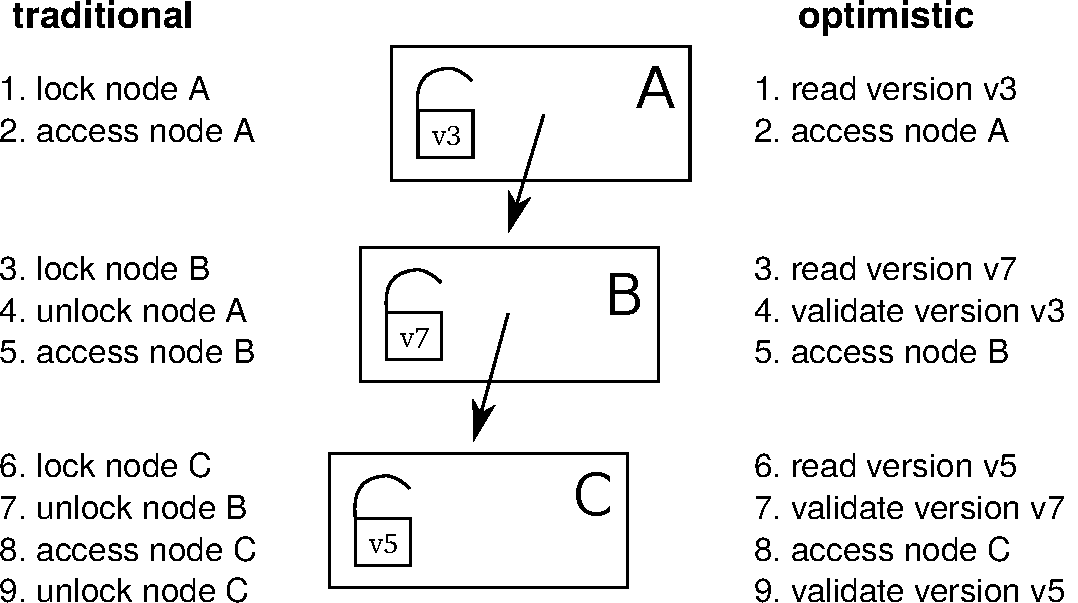
\includegraphics[width=0.65\linewidth]{olcall.pdf}
  \vspace{0.2cm}
  \caption{Comparison of a lookup operation in a 3-level tree using traditional lock coupling (left-hand side) vs.~optimistic lock coupling (right-hand side).}
  \label{fig:olc}
\end{figure}

The traditional and most common lock-based synchronization protocol for B-trees is lock coupling, which interleaves lock acquisitions while holding at most two locks at a time.
If, as we observed earlier, optimistic locks have similar semantics as traditional locks, it is natural to ask whether lock coupling can be combined with optimistic locks.
And indeed the answer is yes: One can almost mechanically translate traditional lock coupling code to optimistic lock coupling code.
This is illustrated in Figure~\ref{fig:olc}, which compares the traversal in a tree of height 3 using traditional and optimistic locks.
As the figure shows, the main difference is that locking is translated to reading the version and that unlocking becomes validation of the previously read version.
This simple change provides efficient lock-free tree traversal without the need to design a complex synchronization protocol.

It is important to emphasize the conceptual simplicity of OLC in comparison to data structures that use custom protocols like the Bw-tree~\cite{DBLP:conf/icde/LevandoskiLS13a}.
To implement lock-free access, the Bw-tree requires an indirection table, delta nodes, complex splitting and merging logic, retry logic, etc.
OLC, on the other hand, can directly be applied to B-trees mostly by adding the appropriate optimistic locking code and without modifying the node layout itself.
Therefore, OpenBw-Tree, an open source implementation of the Bw-tree, requires an order of magnitude more code than a B-tree based on OLC\footnote{Both implementations are available on GitHub: \url{https://github.com/wangziqi2016/index-microbench}}.
Given how difficult it is to develop, validate, and debug lock-free code, simplicity is obviously a major advantage.

\subsection{Correctness Aspects}

\begin{figure}
  % \centering
  %[basicstyle=\normalsize\ttfamily,showstringspaces=false,columns=fullflexible,breaklines=false,breakatwhitespace=true,numbers=none,numberstyle=\small,style=C,keepspaces=true]
\begin{lstlisting}[basicstyle=\ttfamily,language=C++,numbers=left,numberstyle=\small]
std::atomic<BTreeNode*> root;

// search for key in B+tree, returns payload in resultOut
bool lookup(Key key, Value& resultOut) {
   BTreeNode* node = root.load();
   uint64_t nodeVersion = node->readLockOrRestart();
   if (node != root.load()) // make sure the root is still the root
      restart();

   BTreeInner<Key>* parent = nullptr;
   uint64_t parentVersion = 0;

   while (node->isInner()) {
      auto inner = (BTreeInner*)node;

      // unlock parent and make current node the parent
      if (parent)
         parent->readUnlockOrRestart(parentVersion);
      parent = inner;
      parentVersion = nodeVersion;

      // search for next node
      node = inner->findChild(key);
      // validate 'inner' to ensure that 'node' pointer is valid
      inner->checkOrRestart(nodeVersion);
      // now it safe to dereference 'node' pointer (read its version)
      nodeVersion = node->readLockOrRestart();
   }

   // search in leaf and retrieve payload
   auto leaf = (BTreeLeaf*)node;
   bool success = leaf->findValue(key, resultOut);

   // unlock everything
   if (parent)
      parent->readUnlockOrRestart(parentVersion);
   node->readUnlockOrRestart(nodeVersion);

   return success;
}
\end{lstlisting}
  \vspace{0.2cm}
  \caption{B-tree lookup code using OLC. For simplicity, the restart logic is not shown.}
  \label{fig:lookup}
\end{figure}

So far, we have introduced the high-level ideas behind OLC and have stressed its similarity to traditional lock coupling.
Let us now discuss some cases where the close similarity between lock coupling and OLC breaks down.
To make this more concrete, we show the B-tree lookup code in Figure~\ref{fig:lookup}.
In the code, \texttt{readLockOrRestart} reads the lock version and \texttt{readUnlockOrRestart} validates that the read was correct.

One issue with OLC is that any pointer speculatively read from a node may point to invalid memory (if that node is modified concurrently).
Dereferencing such a pointer (e.g., to read its optimistic lock), may cause a segmentation fault or undefined behavior.
In the code shown in Figure~\ref{fig:lookup}, this problem is prevented by the extra check in line 25, which ensures that the read from the node containing the pointer was correct.
Without this additional validation, the code would in line 27 dereference the pointer speculatively read in line 23.
Note that the implementation of \texttt{checkOrRestart} is actually identical to \texttt{readUnlockOrRestart}.
We chose to give it a different name to highlight the fact that this extra check would not be necessary with read/write locks.

Another potential issue with optimistic locks is code that does not terminate.
Code that speculatively accesses a node, like an intra-node binary search, should be written in a way such that it always terminates---even in the presence of concurrent writes.
Otherwise, the validation code that detects the concurrent write will never run.
The binary search of a B-tree, for example, needs to be written in such a way that each comparison makes progress.
For some data structures that do not require loops in the traversal code (like ART) termination is trivially true.

\subsection{Implementation Details}

% implementation, efficiency
To implement an optimistic lock, one can combine the lock and the version counter into a single 64-bit\footnote{Even after subtracting one bit for the lock status, a back-of-the-envelope calculation can show that 63 bits are large enough to never overflow in practice.} word~\cite{artsync}.
A typical read operation will therefore merely consist of reading this version counter atomically.
In C++11 this can be implemented using the \texttt{std::atomic} type.

On x86, atomic reads are cheap because of x86's strong memory order guarantees.
No memory fences are required for sequentially-consistent loads, which are translated (by both GCC and clang) into standard \texttt{MOV} instructions.
Hence, the only effect of \texttt{std::atomic} for loads is preventing instruction re-ordering.
This makes version access and validation cheap.
Acquiring and releasing an optimistic lock in exclusive mode has comparable cost to a traditional lock:
A fairly expensive sequentially-consistent store is needed for acquiring a lock, while a standard \texttt{MOV} suffices for releasing it.
A simple sinlock-based implementation of optimistic locks can be found in the appendix of an earlier paper~\cite{artsync}.

OLC code must be able to handle restarts since validation or lock upgrade can fail due to concurrent writers.
Restarts can easily be implemented by wrapping the data structure operation in a loop (for simplicity not shown in Figure~\ref{fig:lookup}).
Such a loop also enables limiting the number of optimistic retry operations and falling back to pessimistic locking in cases of very heavy contention.
The ability to fall back to traditional locking is a major advantage of OLC in terms of robustness over lock-free approaches, which do not have this option.

In addition to the optimistic shared mode and the exclusive mode, optimistic locks also support a ``shared pessimistic'' mode, which physically acquires the lock in shared mode (allowing multiple concurrent readers but no writers).
This mode is useful for table (or range) scans that touch many tuples on a leaf page (which would otherwise easily abort).
Finally, let us mention that large range scans and table scans, should be broken up into several per-node traversals as is done in the LeanStore~\cite{leanstore} system.

Like all lock-free data structures, but unlike traditional locking and Hardware Transactional Memory~\cite{DBLP:conf/hpca/KarnagelDRLLSL14,DBLP:journals/pvldb/MakreshanskiLS15,htmtkde}, OLC requires care when deleting (and reusing) nodes.
The reason is that a deleting thread can never be sure that a node can be reclaimed because other threads might still be optimistically reading from that node.
Therefore, standard solutions like epoch-based reclamation~\cite{DBLP:conf/sosp/TuZKLM13}, hazard pointers~\cite{DBLP:journals/tpds/Michael04}, or optimized hazard pointers~\cite{DBLP:conf/spaa/BalmauGHZ16} need to be used.
These memory reclamation techniques are, however, largely orthogonal to the synchronization protocol itself.

%-lock-free is not a strong guarantee

\newpage
\section{Evaluation}\label{sec:evaluation}

Let us now experimentally evaluate the overhead and scalability of OLC.
For the experiments, we use an in-memory B+tree implemented in C++11 using templates, which is configured to use nodes of 4096 bytes, random 8 byte keys, and 8 byte payloads.
Based on this B-tree, we compare the following synchronization approaches:
\begin{itemize}
\item an OLC implementation\footnote{An almost identical OLC implementation is available on github: \url{https://github.com/wangziqi2016/index-microbench/tree/master/BTreeOLC}}
\item a variant based on traditional lock coupling and read/write locks
\item the unsynchronized B-tree, which obviously is only correct for read-only workloads but allows measuring the overhead of synchronization
\end{itemize}
Note that earlier work has compared the OLC implementation with a Bw-tree implementation~\cite{buzzword} and other state-of-the-art in-memory index structures.

We use a Haswell EP system with an Intel Xeon E5-2687W v3 CPU, which has 10 cores (20 ``Hyper-Threads'') and 25~MB of L3 cache.
The system is running Ubuntu 18.10 and we use GCC 8.2.0 to compile our code.
The CPU counters are obtained using the Linux perf API\footnote{We use the following convenience wrapper: \url{https://github.com/viktorleis/perfevent}}.

\begin{table}
  \caption{Performance and CPU counters for lookup and insert operations in a B-tree with 100M keys. We perform 100M operations and normalize the CPU counters by that number.}
  \label{tab:overhead}
  \centering
  \begin{tabular}{lrrrrrrr}\toprule
                    &         &        &        & instruc-  & L1     & L3     & branch \\
                    & threads & M op/s & cycles & tions & misses & misses & misses \\\midrule
lookup (no sync.)   & 1       & 1.72   & 2028   & 283     & 39.1   & 14.9   & 16.1   \\
lookup (OLC)        & 1       & 1.65   & 2107   & 370     & 43.9   & 15.1   & 16.7   \\
lookup (lock coup.) & 1       & 1.72   & 2078   & 365     & 42.3   & 16.9   & 15.7   \\\midrule
insert (no sync.)   & 1       & 1.51   & 2286   & 530     & 59.8   & 31.1   & 17.3   \\
insert (OLC)        & 1       & 1.50   & 2303   & 629     & 61.2   & 31.1   & 16.5   \\
insert (lock coup.) & 1       & 1.41   & 2473   & 644     & 61.0   & 31.0   & 17.2   \\\midrule
lookup (no sync.)   & 10      & 15.48  & 2058   & 283     & 38.6   & 15.5   & 16.0   \\
lookup (OLC)        & 10      & 14.60  & 2187   & 370     & 43.8   & 15.8   & 16.8   \\
lookup (lock coup.) & 10      & 5.71   & 5591   & 379     & 54.2   & 17.0   & 14.8   \\\midrule
insert (no sync.)   & 10      & -      & -      & -       & -      & -      & -      \\
insert (OLC)        & 10      & 10.46  & 2940   & 656     & 62.0   & 32.5   & 16.8   \\
insert (lock coup.) & 10      & 7.55   & 4161   & 667     & 75.0   & 28.6   & 16.2   \\
    \bottomrule
\end{tabular}
\end{table}

Table~\ref{tab:overhead} compares the performance and CPU counters for lookup and insert operations in a B-tree with 100M keys.
With {\em single-threaded} execution, we observe that all three approaches have very similar performance.
Adding traditional or optimistic locks to unsynchronized B-tree code results in up to 30\% of additional instructions without affecting single-threaded performance much.

\begin{figure}
  \centering
  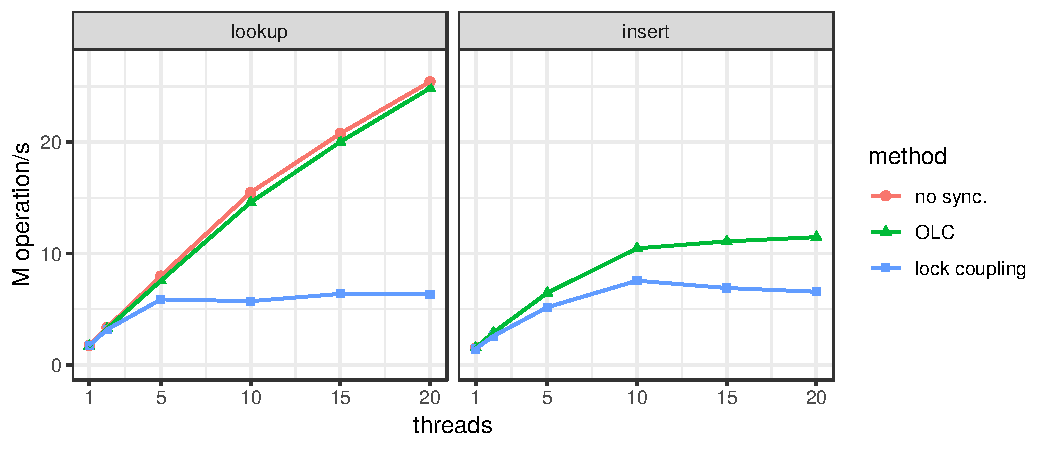
\includegraphics[width=\linewidth]{scale.pdf}
  \vspace{0.2cm}
  \caption{Scalability on 10-core system for B-tree operations (100M values).}
  \label{fig:scale}
\end{figure}

As Figure~\ref{fig:scale} shows, the results change dramatically once we use multiple threads.
For lookup, the scalability of OLC is near-linear up to 20 threads, even though the system has only 10 ``real cores''.
The OLC scalability for insert is also respectable (though not quite as linear because multi-threaded insertion approaches the memory bandwidth of our processor).
The figure also shows that the results of traditional lock coupling with read/write locks are significantly worse than OLC.
With 20 threads, lookup with OLC is 3.9$\times$ faster than traditional lock coupling.

\section{Summary}\label{sec:conc}

Optimistic Lock Coupling (OLC) is an effective synchronization method that combines the simplicity of traditional lock coupling with the superior scalability of lock-free approaches.
OLC is widely applicable and has already been successfully used to synchronize several data structures, including B-trees, binary search trees, and different trie variants.
These features make it highly attractive for modern database systems as well as performance-critical systems software in general.

\begin{thebibliography}{10}

\bibitem{DBLP:conf/spaa/BalmauGHZ16}
O.~Balmau, R.~Guerraoui, M.~Herlihy, and I.~Zablotchi.
\newblock Fast and robust memory reclamation for concurrent data structures.
\newblock In {\em SPAA}, 2016.

\bibitem{DBLP:journals/acta/BayerS77}
R.~Bayer and M.~Schkolnick.
\newblock Concurrency of operations on {B}-trees.
\newblock {\em Acta Informatica}, 9, 1977.

\bibitem{hot}
R.~Binna, E.~Zangerle, M.~Pichl, G.~Specht, and V.~Leis.
\newblock {HOT}: A height optimized trie index for main-memory database
  systems.
\newblock In {\em SIGMOD}, 2018.

\bibitem{DBLP:conf/ppopp/BronsonCCO10}
N.~G. Bronson, J.~Casper, H.~Chafi, and K.~Olukotun.
\newblock A practical concurrent binary search tree.
\newblock In {\em PPOPP}, 2010.

\bibitem{DBLP:conf/vldb/ChaHKK01}
S.~K. Cha, S.~Hwang, K.~Kim, and K.~Kwon.
\newblock Cache-conscious concurrency control of main-memory indexes on
  shared-memory multiprocessor systems.
\newblock In {\em VLDB}, 2001.

\bibitem{intel}
I.~Cutress.
\newblock {Intel} goes for 48-cores: {Cascade-AP} with multi-chip package
  coming soon.
\newblock
  \url{https://www.anandtech.com/show/13535/intel-goes-for-48cores-cascade-ap},
  2018 (accessed January, 2019).

\bibitem{DBLP:conf/cidr/FaleiroA17}
J.~M. Faleiro and D.~J. Abadi.
\newblock Latch-free synchronization in database systems: Silver bullet or
  fool's gold?
\newblock In {\em CIDR}, 2017.

\bibitem{DBLP:journals/ftdb/Graefe11}
G.~Graefe.
\newblock Modern {B}-tree techniques.
\newblock {\em Foundations and Trends in Databases}, 3(4), 2011.

\bibitem{DBLP:conf/hpca/KarnagelDRLLSL14}
T.~Karnagel, R.~Dementiev, R.~Rajwar, K.~Lai, T.~Legler, B.~Schlegel, and
  W.~Lehner.
\newblock Improving in-memory database index performance with
  {Intel}\({}^{\mbox{{\textregistered}}}\) transactional synchronization
  extensions.
\newblock In {\em HPCA}, 2014.

\bibitem{DBLP:journals/tods/LehmanY81}
P.~L. Lehman and S.~B. Yao.
\newblock Efficient locking for concurrent operations on {B}-trees.
\newblock {\em {ACM} Trans. Database Syst.}, 6(4), 1981.

\bibitem{leanstore}
V.~Leis, M.~Haubenschild, A.~Kemper, and T.~Neumann.
\newblock Leanstore: In-memory data management beyond main memory.
\newblock In {\em ICDE}, 2018.

\bibitem{art}
V.~Leis, A.~Kemper, and T.~Neumann.
\newblock The adaptive radix tree: {ARTful} indexing for main-memory databases.
\newblock In {\em ICDE}, 2013.

\bibitem{htmtkde}
V.~Leis, A.~Kemper, and T.~Neumann.
\newblock Scaling {HTM}-supported database transactions to many cores.
\newblock {\em {IEEE} Trans. Knowl. Data Eng.}, 28(2), 2016.

\bibitem{artsync}
V.~Leis, F.~Scheibner, A.~Kemper, and T.~Neumann.
\newblock The {ART} of practical synchronization.
\newblock In {\em DaMoN}, 2016.

\bibitem{DBLP:conf/icde/LevandoskiLS13a}
J.~J. Levandoski, D.~B. Lomet, and S.~Sengupta.
\newblock The {Bw}-tree: A {B}-tree for new hardware platforms.
\newblock In {\em ICDE}, 2013.

\bibitem{DBLP:journals/pvldb/MakreshanskiLS15}
D.~Makreshanski, J.~J. Levandoski, and R.~Stutsman.
\newblock To lock, swap, or elide: On the interplay of hardware transactional
  memory and lock-free indexing.
\newblock {\em {PVLDB}}, 8(11), 2015.

\bibitem{DBLP:dblp_conf/eurosys/MaoKM12}
Y.~Mao, E.~Kohler, and R.~T. Morris.
\newblock Cache craftiness for fast multicore key-value storage.
\newblock In {\em EuroSys}, 2012.

\bibitem{DBLP:journals/tpds/Michael04}
M.~M. Michael.
\newblock Hazard pointers: Safe memory reclamation for lock-free objects.
\newblock {\em {IEEE} Trans. Parallel Distrib. Syst.}, 15(6), 2004.

\bibitem{DBLP:journals/jacm/ShalevS06}
O.~Shalev and N.~Shavit.
\newblock Split-ordered lists: Lock-free extensible hash tables.
\newblock {\em J. {ACM}}, 53(3), 2006.

\bibitem{amd}
A.~Shilov.
\newblock {AMD} previews {EPYC} ‘{Rome}’ processor: Up to 64 {Zen} 2 cores.
\newblock
  \url{https://www.anandtech.com/show/13561/amd-previews-epyc-rome-processor-up-to-64-zen-2-cores},
  2018 (accessed January, 2019).

\bibitem{DBLP:conf/sosp/TuZKLM13}
S.~Tu, W.~Zheng, E.~Kohler, B.~Liskov, and S.~Madden.
\newblock Speedy transactions in multicore in-memory databases.
\newblock In {\em SOSP}, 2013.

\bibitem{buzzword}
Z.~Wang, A.~Pavlo, H.~Lim, V.~Leis, H.~Zhang, M.~Kaminsky, and D.~Andersen.
\newblock Building a {Bw}-tree takes more than just buzz words.
\newblock In {\em SIGMOD}, 2018.

\end{thebibliography}


%\bibliographystyle{abbrv}
%\bibliography{main}

\end{document}

\end{article}

\begin{article}
{Knowledge Graph Comparative Reasoning for Fact Checking: Problem Definition and Algorithms}
{Lihui Liu*, Ruining Zhao*,  Boxin Du, Yi Ren Fung, Heng Ji, Jiejun Xu, and Hanghang Tong}
\pdfminorversion=5
\documentclass[11pt]{article}
\usepackage{deauthor,times,graphicx,caption,microtype}
\usepackage{hyperref}
\usepackage{listings}
\usepackage{booktabs}

\begin{document}

\title{Optimistic Lock Coupling: A Scalable and Efficient General-Purpose Synchronization Method}

\author{Viktor Leis, Michael Haubenschild\raisebox{0.9ex}{$\ast$}, Thomas Neumann\\ Technische Universit{\"a}t M{\"u}nchen \hspace{0.7cm} Tableau Software\raisebox{0.9ex}{$\ast$} \\ {\{leis,neumann\}{@}in.tum.de} \hspace{0.7cm} {mhaubenschild{@}tableau.com\raisebox{0.9ex}{$\ast$}}}

\maketitle

\begin{abstract}
As the number of cores on commodity processors continues to increase, scalability becomes more and more crucial for overall performance.
Scalable and efficient concurrent data structures are particularly important, as these are often the building blocks of parallel algorithms.
Unfortunately, traditional synchronization techniques based on fine-grained locking have been shown to be unscalable on modern multi-core CPUs.
Lock-free data structures, on the other hand, are extremely difficult to design and often incur significant overhead.

In this work, we make the case for Optimistic Lock Coupling as a practical alternative to both traditional locking and the lock-free approach.
We show that Optimistic Lock Coupling is highly scalable and almost as simple to implement as traditional lock coupling.
Another important advantage is that it is easily applicable to most tree-like data structures.
We therefore argue that Optimistic Lock Coupling, rather than a complex and error-prone custom synchronization protocol, should be the default choice for performance-critical data structures.
\end{abstract}

\section{Introduction}

% more and more cores
Today, Intel's commodity server processors have up to 28 cores and its upcoming microarchitecture will have up to 48 cores per socket~\cite{intel}.
Similarly, AMD currently stands at 32 cores and this number is expected to double in the next generation~\cite{amd}.
Since both platforms support simultaneous multithreading (also known as hyperthreading), affordable commodity servers (with up to two sockets) will soon routinely have between 100 and 200 hardware threads.

% data structure scalability is important
With such a high degree of hardware parallelism, efficient data processing crucially depends on how well concurrent data structures scale.
Internally, database systems use a plethora of data structures like table heaps, internal work queues, and, most importantly, index structures.
Any of these can easily become a scalability (and therefore overall performance) bottleneck on many-core CPUs.

% traditional synchronization: fine-grained locks, slow, cache invalidation
Traditionally, database systems synchronize internal data structures using fine-grained reader/writer locks\footnote{In this work, we focus on data structure synchronization rather than high-level transaction semantics and therefore use the term {\em lock} for what would typically be called {\em latch} in the database literature. We thus follow common computer science (rather than database) terminology.}.
Unfortunately, while fine-grained locking makes lock contention unlikely, it still results in bad scalability because lock acquisition and release require writing to shared memory.
Due to the way cache coherency is implemented on modern multi-core CPUs, these writes cause additional cache misses\footnote{The cache coherency protocol ensures that all copies of a cache line on other cores are invalidated before the write can proceed.} and the cache line containing the lock's internal data becomes a point of physical contention.
As a result, any frequently-accessed lock (e.g., the lock of the root node of a B-tree) severely limits scalability.

% lock-free bw-tree: no more latches, but indirections, extremely complex
Lock-free data structures like the Bw-tree~\cite{DBLP:conf/icde/LevandoskiLS13a} (a lock-free B-tree variant) or the Split-Ordered List~\cite{DBLP:journals/jacm/ShalevS06} (a lock-free hash table) do not acquire any locks and therefore generally scale much better than locking-based approaches (in particular for read-mostly workloads).
However, lock-free synchronization has other downsides:
First, it is very difficult and results in extremely complex and error-prone code (when compared to locking).
Second, because the functionality of atomic primitives provided by the hardware (e.g., atomically compare-and-swap 8 bytes) is limited, complex operations require additional indirections within the data structure.
For example, the Bw-tree requires an indirection table and the Split-Ordered List requires ``dummy nodes'', resulting in overhead due to additional cache misses.

% OLC for the win
In this paper we make the case for {\em Optimistic Lock Coupling (OLC)}, a synchronization method that combines some of the best properties of lock-based and lock-free synchronization.
OLC utilizes a special lock type that can be used in two modes:
The first mode is similar to a traditional mutex and excludes other threads by physically acquiring the underlying lock.
In the second mode, reads can proceed optimistically by validating a version counter that is embedded in the lock (similar to optimistic concurrency control).
The first mode is typically used by writers and the second mode by readers.
Besides this special lock type, OLC is based on the observation that optimistic lock validations can be interleaved/coupled---similar to the pair-wise interleaved lock acquisition of traditional lock coupling.
Hence, the name Optimistic Lock Coupling.

OLC has a number of desirable features:
\begin{itemize}
\item By reducing the number of writes to shared memory locations and thereby avoiding cache invalidations, it {\bf scales well} for most workloads.
\item In comparison to unsynchronized code, it requires few additional CPU instructions making it {\bf efficient}.
\item OLC is {\bf widely applicable} to different data structures. It has already been successfully used for synchronizing binary search trees~\cite{DBLP:conf/ppopp/BronsonCCO10}, tries~\cite{artsync}, trie/B-tree hybrids~\cite{DBLP:dblp_conf/eurosys/MaoKM12}, and B-trees~\cite{buzzword}.
\item In comparison to the lock-free paradigm, it is also {\bf easy to use} and requires few modifications to existing, single-threaded data structures.
\end{itemize}
Despite these positive features and its simplicity, OLC is not yet widely known.
The goal of this paper is therefore to popularize this simple idea and to make a case for it.
We argue that OLC deserves to be widely known.
It is a good default synchronization paradigm---more complex, data structure-specific protocols are seldom beneficial.

The rest of the paper is organized as follows.
Section~\ref{sec:related} discusses related work, tracing the history of OLC and its underlying ideas in the literature.
The core of the paper is Section~\ref{sec:olc}, which describes the ideas behind OLC and how it can be used to synchronize complex data structures.
In Section~\ref{sec:evaluation} we experimentally show that OLC has low overhead and scales well when used to synchronize an in-memory B-tree.
We summarize the paper in Section~\ref{sec:conc}.

\newpage
\section{Related Work}\label{sec:related}

Lock coupling has been proposed as a method for allowing concurrent operations on B-trees in 1977~\cite{DBLP:journals/acta/BayerS77}.
This traditional and still widely-used method, described in detail in Graefe's B-tree survey~\cite{DBLP:journals/ftdb/Graefe11}, is also called ``latch coupling'', ``hand-over-hand locking'', and ``crabbing''.
Because at most two locks are held at-a-time during tree traversal, this technique seemingly allows for a high degree of parallelism---in particular if read/write locks are used to enable inner nodes to be locked in shared mode.
However, as we show in Section~\ref{sec:evaluation}, on modern hardware lock acquisition (even in shared mode) results in suboptimal scalability.

An early alternative from 1981 is a B-tree variant called B-link tree~\cite{DBLP:journals/tods/LehmanY81}, which only holds a single lock at a time.
It is based on the observation that between the release of the parent lock and the acquisition of the child lock, the only ``dangerous'' thing that could have happened is the split of a child node (assuming one does not implement merge operations).
Thus, when a split happens, the key being searched might end up on a neighboring node to the right of the current child node.
A B-link tree traversal therefore detects this condition and, if needed, transparently proceeds to the neighboring node.
Releasing the parent lock early is highly beneficial when the child node needs to be fetched from disk.
For in-memory workloads, however, the B-link tree has the same scalability issues as lock coupling (it acquires just as many locks).

The next major advance, Optimistic Latch-Free Index Traversal (OLFIT)~\cite{DBLP:conf/vldb/ChaHKK01}, was proposed in 2001.
OLFIT introduced the idea of a combined lock/update counter, which we call {\em optimistic lock}. % , for lack of a better name,
Based on these per-node optimistic locks and the synchronization protocol of the B-link tree, OLFIT finally achieves good scalability on parallel processors.
The OLFIT protocol is fairly complex, as it requires both the non-trivial B-link protocol and optimistic locks.
Furthermore, like the B-link tree protocol, it does not support merging nodes, and is specific to B-trees (cannot easily be applied to other data structures).

In the following two decades, the growth of main-memory capacity led to much research into other data structures besides the venerable B-tree.
Particularly relevant for our discussion is Bronson et al.'s~\cite{DBLP:conf/ppopp/BronsonCCO10} concurrent binary search tree, which is based on optimistic version validation and has a sophisticated, data structure-specific synchronization protocol.
To the best of our knowledge, this 2010 paper is the first that, as part of its protocol, interleaves version validation across nodes---rather than validating each node separately like OLFIT.
In that paper, this idea is called ``hand-over-hand, optimistic validation'', while we prefer the term Optimistic Lock Coupling to highlight the close resemblance to traditional lock coupling.
Similarly, Mao et al.'s~\cite{DBLP:dblp_conf/eurosys/MaoKM12} Masstree (a concurrent hybrid trie/B-tree) is also based on the same ideas, but again uses them as part of a more complex protocol.

The Adaptive Radix Tree (ART)~\cite{art} is another recent in-memory data structure, which we proposed in 2013.
In contrast to the two data structures just mentioned, it was originally designed with single-threaded performance in mind without supporting concurrency.
To add support for concurrency, we initially started designing a custom protocol called Read-Optimized Write Exclusion (ROWEX)~\cite{artsync}, which turned out to be non-trivial and requires modifications of the underlying data structure\footnote{Note that ROWEX is already easier to apply to existing data structures than the lock-free approach. The difficulty depends on the data structure. Applying ROWEX is hard for B-trees with sorted keys and fairly easy for copy-on-write data structures like the Height Optimized Trie~\cite{hot}---with ART being somewhere in the middle.}.
However, fairly late in the project, we also realized, that OLC {\em alone} (rather than as part of a more complex protocol) is sufficient to synchronize ART.
No other changes to the data structure were necessary.
Both approaches were published and experimentally evaluated in a followup paper~\cite{artsync}, which shows that, despite its simplicity, OLC is efficient, scalable, and generally outperforms ROWEX.

Similar results were recently published regarding B-trees~\cite{buzzword}.
In this experimental study a simple OLC-based synchronization outperformed the Bw-tree~\cite{DBLP:conf/icde/LevandoskiLS13a}, a complex lock-free synchronization approach.
Another recent paper shows that for write-intensive workloads, locking often performs better than lock-free synchronization~\cite{DBLP:conf/cidr/FaleiroA17}.
These experiences indicate that OLC is a general-purpose synchronization paradigm and motivate the current paper.

%foster b-tree\cite{DBLP:journals/tods/GraefeKK12}
%Shasha theory~\cite{DBLP:journals/tods/ShashaG88}

\section{Optimistic Lock Coupling}\label{sec:olc}

% locks suck
The standard technique for inter-thread synchronization is mutual exclusion using fine-grained locks.
In a B-tree, for example, every node usually has its own associated lock, which is acquired before accessing that node.
The problem of locking on modern multi- and many-core processors is that lock acquisition and release require writing to the shared memory location that implements the lock.
This write causes exclusive ownership of the underlying cache line and invalidates copies of it on all other processor cores.
For hierarchical, tree-like data structures, the lock of the root node becomes a point of physical contention---even in read-only workloads and even when read/write locks are used.
Depending on the specific data structure, number of cores, cache coherency protocol implementation, cache topology, whether Non-Uniform Memory Access (NUMA) is used, locking can even result in multi-threaded performance that is worse than single-threaded execution.

% in b-trees this happens very much
The inherent pessimism of locking is particularly unfortunate for B-trees:
Despite the fact that logical modifications of the root node are very infrequent, every B-tree operation must lock the root node during tree traversal\footnote{To a lesser extent this obviously applies to all inner nodes, not just the root.}.
Even the vast majority of update operations (with the exception of splits and merges), only modify a single leaf node.
These observations indicate that a more optimistic approach, which does not require locking inner nodes, would be very beneficial for B-trees.

\subsection{Optimistic Locks}

% optimism to the rescue
As the name indicates, optimistic locks try to solve the scalability issues of traditional locks using an optimistic approach.
Instead of always physically acquiring locks, even for nodes that are unlikely to be modified simultaneously, after-the-fact validation is used to detect conflicts.
This is done by augmenting each lock with a version/update counter that is incremented on every modification.
Using this version counter, readers can optimistically proceed before validating that the version did not change to ensure that the read was safe.
If validation fails, the operation is restarted.

% details on opt locks
Using optimistic locks, a read-only node access (i.e., the majority of all operations in a B-tree) does not acquire the lock and does not increment the version counter.
Instead, it performs the following steps:
\begin{enumerate}
\item read lock version (restart if lock is not free)
\item access node
\item read the version again and validate that it has not changed in the meantime
\end{enumerate}
If the last step (the validation) fails, the operation has to be restarted.
Write operations, on the other hand, are more similar to traditional locking:
\begin{enumerate}
\item acquire lock (wait if necessary)
\item access/write to node
\item increment version and unlock node
\end{enumerate}
Writes can therefore protect a node from other writes.

% similar to locks
As we observed in an earlier paper~\cite{artsync}, because of similar semantics, optimistic locks can be hidden behind an API very similar to traditional read/write locks.
Both approaches have an exclusive lock mode, and acquiring a traditional lock in shared mode is analogous to optimistic version validation.
Furthermore, like with some implementations of traditional read/write locks, optimistic locks allow upgrading a shared lock to an exclusive lock.
Lock upgrades are, for example, used to avoid most B-tree update operations from having to lock inner nodes.
In our experience, the close resemblance of optimistic and traditional locks simplifies the reasoning about optimistic locks;
one can apply similar thinking as in traditional lock-based protocols.

\subsection{Lock Coupling with Optimistic Locks}

\begin{figure}
  \centering
  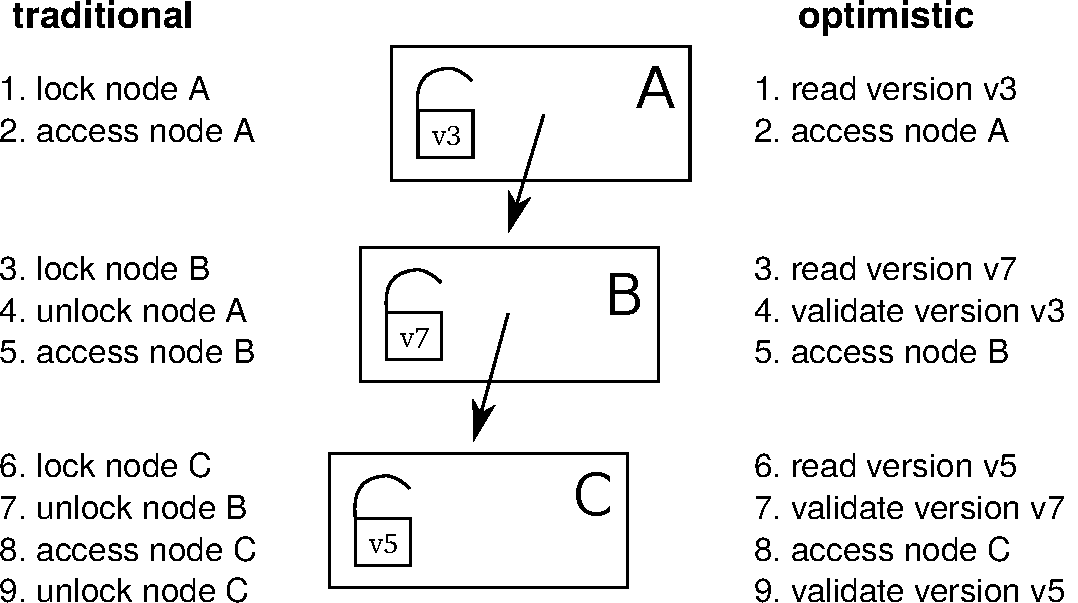
\includegraphics[width=0.65\linewidth]{olcall.pdf}
  \vspace{0.2cm}
  \caption{Comparison of a lookup operation in a 3-level tree using traditional lock coupling (left-hand side) vs.~optimistic lock coupling (right-hand side).}
  \label{fig:olc}
\end{figure}

The traditional and most common lock-based synchronization protocol for B-trees is lock coupling, which interleaves lock acquisitions while holding at most two locks at a time.
If, as we observed earlier, optimistic locks have similar semantics as traditional locks, it is natural to ask whether lock coupling can be combined with optimistic locks.
And indeed the answer is yes: One can almost mechanically translate traditional lock coupling code to optimistic lock coupling code.
This is illustrated in Figure~\ref{fig:olc}, which compares the traversal in a tree of height 3 using traditional and optimistic locks.
As the figure shows, the main difference is that locking is translated to reading the version and that unlocking becomes validation of the previously read version.
This simple change provides efficient lock-free tree traversal without the need to design a complex synchronization protocol.

It is important to emphasize the conceptual simplicity of OLC in comparison to data structures that use custom protocols like the Bw-tree~\cite{DBLP:conf/icde/LevandoskiLS13a}.
To implement lock-free access, the Bw-tree requires an indirection table, delta nodes, complex splitting and merging logic, retry logic, etc.
OLC, on the other hand, can directly be applied to B-trees mostly by adding the appropriate optimistic locking code and without modifying the node layout itself.
Therefore, OpenBw-Tree, an open source implementation of the Bw-tree, requires an order of magnitude more code than a B-tree based on OLC\footnote{Both implementations are available on GitHub: \url{https://github.com/wangziqi2016/index-microbench}}.
Given how difficult it is to develop, validate, and debug lock-free code, simplicity is obviously a major advantage.

\subsection{Correctness Aspects}

\begin{figure}
  % \centering
  %[basicstyle=\normalsize\ttfamily,showstringspaces=false,columns=fullflexible,breaklines=false,breakatwhitespace=true,numbers=none,numberstyle=\small,style=C,keepspaces=true]
\begin{lstlisting}[basicstyle=\ttfamily,language=C++,numbers=left,numberstyle=\small]
std::atomic<BTreeNode*> root;

// search for key in B+tree, returns payload in resultOut
bool lookup(Key key, Value& resultOut) {
   BTreeNode* node = root.load();
   uint64_t nodeVersion = node->readLockOrRestart();
   if (node != root.load()) // make sure the root is still the root
      restart();

   BTreeInner<Key>* parent = nullptr;
   uint64_t parentVersion = 0;

   while (node->isInner()) {
      auto inner = (BTreeInner*)node;

      // unlock parent and make current node the parent
      if (parent)
         parent->readUnlockOrRestart(parentVersion);
      parent = inner;
      parentVersion = nodeVersion;

      // search for next node
      node = inner->findChild(key);
      // validate 'inner' to ensure that 'node' pointer is valid
      inner->checkOrRestart(nodeVersion);
      // now it safe to dereference 'node' pointer (read its version)
      nodeVersion = node->readLockOrRestart();
   }

   // search in leaf and retrieve payload
   auto leaf = (BTreeLeaf*)node;
   bool success = leaf->findValue(key, resultOut);

   // unlock everything
   if (parent)
      parent->readUnlockOrRestart(parentVersion);
   node->readUnlockOrRestart(nodeVersion);

   return success;
}
\end{lstlisting}
  \vspace{0.2cm}
  \caption{B-tree lookup code using OLC. For simplicity, the restart logic is not shown.}
  \label{fig:lookup}
\end{figure}

So far, we have introduced the high-level ideas behind OLC and have stressed its similarity to traditional lock coupling.
Let us now discuss some cases where the close similarity between lock coupling and OLC breaks down.
To make this more concrete, we show the B-tree lookup code in Figure~\ref{fig:lookup}.
In the code, \texttt{readLockOrRestart} reads the lock version and \texttt{readUnlockOrRestart} validates that the read was correct.

One issue with OLC is that any pointer speculatively read from a node may point to invalid memory (if that node is modified concurrently).
Dereferencing such a pointer (e.g., to read its optimistic lock), may cause a segmentation fault or undefined behavior.
In the code shown in Figure~\ref{fig:lookup}, this problem is prevented by the extra check in line 25, which ensures that the read from the node containing the pointer was correct.
Without this additional validation, the code would in line 27 dereference the pointer speculatively read in line 23.
Note that the implementation of \texttt{checkOrRestart} is actually identical to \texttt{readUnlockOrRestart}.
We chose to give it a different name to highlight the fact that this extra check would not be necessary with read/write locks.

Another potential issue with optimistic locks is code that does not terminate.
Code that speculatively accesses a node, like an intra-node binary search, should be written in a way such that it always terminates---even in the presence of concurrent writes.
Otherwise, the validation code that detects the concurrent write will never run.
The binary search of a B-tree, for example, needs to be written in such a way that each comparison makes progress.
For some data structures that do not require loops in the traversal code (like ART) termination is trivially true.

\subsection{Implementation Details}

% implementation, efficiency
To implement an optimistic lock, one can combine the lock and the version counter into a single 64-bit\footnote{Even after subtracting one bit for the lock status, a back-of-the-envelope calculation can show that 63 bits are large enough to never overflow in practice.} word~\cite{artsync}.
A typical read operation will therefore merely consist of reading this version counter atomically.
In C++11 this can be implemented using the \texttt{std::atomic} type.

On x86, atomic reads are cheap because of x86's strong memory order guarantees.
No memory fences are required for sequentially-consistent loads, which are translated (by both GCC and clang) into standard \texttt{MOV} instructions.
Hence, the only effect of \texttt{std::atomic} for loads is preventing instruction re-ordering.
This makes version access and validation cheap.
Acquiring and releasing an optimistic lock in exclusive mode has comparable cost to a traditional lock:
A fairly expensive sequentially-consistent store is needed for acquiring a lock, while a standard \texttt{MOV} suffices for releasing it.
A simple sinlock-based implementation of optimistic locks can be found in the appendix of an earlier paper~\cite{artsync}.

OLC code must be able to handle restarts since validation or lock upgrade can fail due to concurrent writers.
Restarts can easily be implemented by wrapping the data structure operation in a loop (for simplicity not shown in Figure~\ref{fig:lookup}).
Such a loop also enables limiting the number of optimistic retry operations and falling back to pessimistic locking in cases of very heavy contention.
The ability to fall back to traditional locking is a major advantage of OLC in terms of robustness over lock-free approaches, which do not have this option.

In addition to the optimistic shared mode and the exclusive mode, optimistic locks also support a ``shared pessimistic'' mode, which physically acquires the lock in shared mode (allowing multiple concurrent readers but no writers).
This mode is useful for table (or range) scans that touch many tuples on a leaf page (which would otherwise easily abort).
Finally, let us mention that large range scans and table scans, should be broken up into several per-node traversals as is done in the LeanStore~\cite{leanstore} system.

Like all lock-free data structures, but unlike traditional locking and Hardware Transactional Memory~\cite{DBLP:conf/hpca/KarnagelDRLLSL14,DBLP:journals/pvldb/MakreshanskiLS15,htmtkde}, OLC requires care when deleting (and reusing) nodes.
The reason is that a deleting thread can never be sure that a node can be reclaimed because other threads might still be optimistically reading from that node.
Therefore, standard solutions like epoch-based reclamation~\cite{DBLP:conf/sosp/TuZKLM13}, hazard pointers~\cite{DBLP:journals/tpds/Michael04}, or optimized hazard pointers~\cite{DBLP:conf/spaa/BalmauGHZ16} need to be used.
These memory reclamation techniques are, however, largely orthogonal to the synchronization protocol itself.

%-lock-free is not a strong guarantee

\newpage
\section{Evaluation}\label{sec:evaluation}

Let us now experimentally evaluate the overhead and scalability of OLC.
For the experiments, we use an in-memory B+tree implemented in C++11 using templates, which is configured to use nodes of 4096 bytes, random 8 byte keys, and 8 byte payloads.
Based on this B-tree, we compare the following synchronization approaches:
\begin{itemize}
\item an OLC implementation\footnote{An almost identical OLC implementation is available on github: \url{https://github.com/wangziqi2016/index-microbench/tree/master/BTreeOLC}}
\item a variant based on traditional lock coupling and read/write locks
\item the unsynchronized B-tree, which obviously is only correct for read-only workloads but allows measuring the overhead of synchronization
\end{itemize}
Note that earlier work has compared the OLC implementation with a Bw-tree implementation~\cite{buzzword} and other state-of-the-art in-memory index structures.

We use a Haswell EP system with an Intel Xeon E5-2687W v3 CPU, which has 10 cores (20 ``Hyper-Threads'') and 25~MB of L3 cache.
The system is running Ubuntu 18.10 and we use GCC 8.2.0 to compile our code.
The CPU counters are obtained using the Linux perf API\footnote{We use the following convenience wrapper: \url{https://github.com/viktorleis/perfevent}}.

\begin{table}
  \caption{Performance and CPU counters for lookup and insert operations in a B-tree with 100M keys. We perform 100M operations and normalize the CPU counters by that number.}
  \label{tab:overhead}
  \centering
  \begin{tabular}{lrrrrrrr}\toprule
                    &         &        &        & instruc-  & L1     & L3     & branch \\
                    & threads & M op/s & cycles & tions & misses & misses & misses \\\midrule
lookup (no sync.)   & 1       & 1.72   & 2028   & 283     & 39.1   & 14.9   & 16.1   \\
lookup (OLC)        & 1       & 1.65   & 2107   & 370     & 43.9   & 15.1   & 16.7   \\
lookup (lock coup.) & 1       & 1.72   & 2078   & 365     & 42.3   & 16.9   & 15.7   \\\midrule
insert (no sync.)   & 1       & 1.51   & 2286   & 530     & 59.8   & 31.1   & 17.3   \\
insert (OLC)        & 1       & 1.50   & 2303   & 629     & 61.2   & 31.1   & 16.5   \\
insert (lock coup.) & 1       & 1.41   & 2473   & 644     & 61.0   & 31.0   & 17.2   \\\midrule
lookup (no sync.)   & 10      & 15.48  & 2058   & 283     & 38.6   & 15.5   & 16.0   \\
lookup (OLC)        & 10      & 14.60  & 2187   & 370     & 43.8   & 15.8   & 16.8   \\
lookup (lock coup.) & 10      & 5.71   & 5591   & 379     & 54.2   & 17.0   & 14.8   \\\midrule
insert (no sync.)   & 10      & -      & -      & -       & -      & -      & -      \\
insert (OLC)        & 10      & 10.46  & 2940   & 656     & 62.0   & 32.5   & 16.8   \\
insert (lock coup.) & 10      & 7.55   & 4161   & 667     & 75.0   & 28.6   & 16.2   \\
    \bottomrule
\end{tabular}
\end{table}

Table~\ref{tab:overhead} compares the performance and CPU counters for lookup and insert operations in a B-tree with 100M keys.
With {\em single-threaded} execution, we observe that all three approaches have very similar performance.
Adding traditional or optimistic locks to unsynchronized B-tree code results in up to 30\% of additional instructions without affecting single-threaded performance much.

\begin{figure}
  \centering
  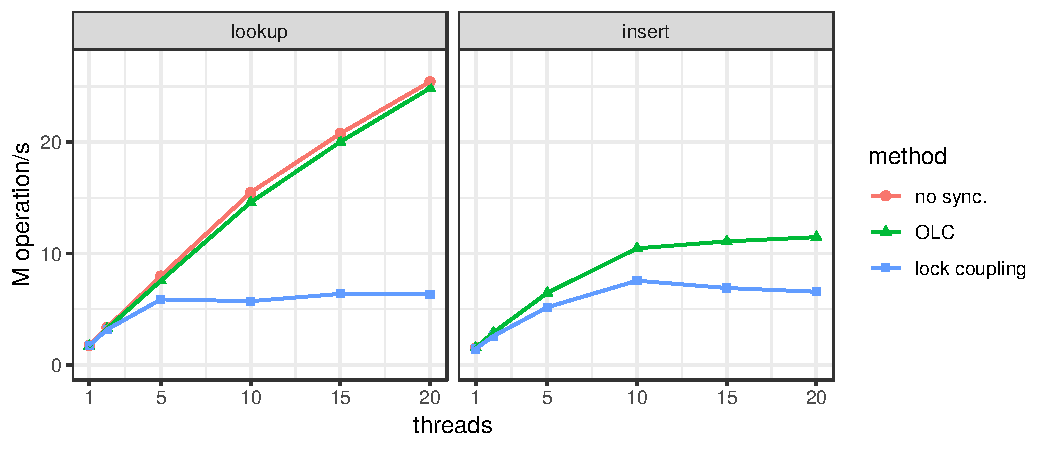
\includegraphics[width=\linewidth]{scale.pdf}
  \vspace{0.2cm}
  \caption{Scalability on 10-core system for B-tree operations (100M values).}
  \label{fig:scale}
\end{figure}

As Figure~\ref{fig:scale} shows, the results change dramatically once we use multiple threads.
For lookup, the scalability of OLC is near-linear up to 20 threads, even though the system has only 10 ``real cores''.
The OLC scalability for insert is also respectable (though not quite as linear because multi-threaded insertion approaches the memory bandwidth of our processor).
The figure also shows that the results of traditional lock coupling with read/write locks are significantly worse than OLC.
With 20 threads, lookup with OLC is 3.9$\times$ faster than traditional lock coupling.

\section{Summary}\label{sec:conc}

Optimistic Lock Coupling (OLC) is an effective synchronization method that combines the simplicity of traditional lock coupling with the superior scalability of lock-free approaches.
OLC is widely applicable and has already been successfully used to synchronize several data structures, including B-trees, binary search trees, and different trie variants.
These features make it highly attractive for modern database systems as well as performance-critical systems software in general.

\begin{thebibliography}{10}

\bibitem{DBLP:conf/spaa/BalmauGHZ16}
O.~Balmau, R.~Guerraoui, M.~Herlihy, and I.~Zablotchi.
\newblock Fast and robust memory reclamation for concurrent data structures.
\newblock In {\em SPAA}, 2016.

\bibitem{DBLP:journals/acta/BayerS77}
R.~Bayer and M.~Schkolnick.
\newblock Concurrency of operations on {B}-trees.
\newblock {\em Acta Informatica}, 9, 1977.

\bibitem{hot}
R.~Binna, E.~Zangerle, M.~Pichl, G.~Specht, and V.~Leis.
\newblock {HOT}: A height optimized trie index for main-memory database
  systems.
\newblock In {\em SIGMOD}, 2018.

\bibitem{DBLP:conf/ppopp/BronsonCCO10}
N.~G. Bronson, J.~Casper, H.~Chafi, and K.~Olukotun.
\newblock A practical concurrent binary search tree.
\newblock In {\em PPOPP}, 2010.

\bibitem{DBLP:conf/vldb/ChaHKK01}
S.~K. Cha, S.~Hwang, K.~Kim, and K.~Kwon.
\newblock Cache-conscious concurrency control of main-memory indexes on
  shared-memory multiprocessor systems.
\newblock In {\em VLDB}, 2001.

\bibitem{intel}
I.~Cutress.
\newblock {Intel} goes for 48-cores: {Cascade-AP} with multi-chip package
  coming soon.
\newblock
  \url{https://www.anandtech.com/show/13535/intel-goes-for-48cores-cascade-ap},
  2018 (accessed January, 2019).

\bibitem{DBLP:conf/cidr/FaleiroA17}
J.~M. Faleiro and D.~J. Abadi.
\newblock Latch-free synchronization in database systems: Silver bullet or
  fool's gold?
\newblock In {\em CIDR}, 2017.

\bibitem{DBLP:journals/ftdb/Graefe11}
G.~Graefe.
\newblock Modern {B}-tree techniques.
\newblock {\em Foundations and Trends in Databases}, 3(4), 2011.

\bibitem{DBLP:conf/hpca/KarnagelDRLLSL14}
T.~Karnagel, R.~Dementiev, R.~Rajwar, K.~Lai, T.~Legler, B.~Schlegel, and
  W.~Lehner.
\newblock Improving in-memory database index performance with
  {Intel}\({}^{\mbox{{\textregistered}}}\) transactional synchronization
  extensions.
\newblock In {\em HPCA}, 2014.

\bibitem{DBLP:journals/tods/LehmanY81}
P.~L. Lehman and S.~B. Yao.
\newblock Efficient locking for concurrent operations on {B}-trees.
\newblock {\em {ACM} Trans. Database Syst.}, 6(4), 1981.

\bibitem{leanstore}
V.~Leis, M.~Haubenschild, A.~Kemper, and T.~Neumann.
\newblock Leanstore: In-memory data management beyond main memory.
\newblock In {\em ICDE}, 2018.

\bibitem{art}
V.~Leis, A.~Kemper, and T.~Neumann.
\newblock The adaptive radix tree: {ARTful} indexing for main-memory databases.
\newblock In {\em ICDE}, 2013.

\bibitem{htmtkde}
V.~Leis, A.~Kemper, and T.~Neumann.
\newblock Scaling {HTM}-supported database transactions to many cores.
\newblock {\em {IEEE} Trans. Knowl. Data Eng.}, 28(2), 2016.

\bibitem{artsync}
V.~Leis, F.~Scheibner, A.~Kemper, and T.~Neumann.
\newblock The {ART} of practical synchronization.
\newblock In {\em DaMoN}, 2016.

\bibitem{DBLP:conf/icde/LevandoskiLS13a}
J.~J. Levandoski, D.~B. Lomet, and S.~Sengupta.
\newblock The {Bw}-tree: A {B}-tree for new hardware platforms.
\newblock In {\em ICDE}, 2013.

\bibitem{DBLP:journals/pvldb/MakreshanskiLS15}
D.~Makreshanski, J.~J. Levandoski, and R.~Stutsman.
\newblock To lock, swap, or elide: On the interplay of hardware transactional
  memory and lock-free indexing.
\newblock {\em {PVLDB}}, 8(11), 2015.

\bibitem{DBLP:dblp_conf/eurosys/MaoKM12}
Y.~Mao, E.~Kohler, and R.~T. Morris.
\newblock Cache craftiness for fast multicore key-value storage.
\newblock In {\em EuroSys}, 2012.

\bibitem{DBLP:journals/tpds/Michael04}
M.~M. Michael.
\newblock Hazard pointers: Safe memory reclamation for lock-free objects.
\newblock {\em {IEEE} Trans. Parallel Distrib. Syst.}, 15(6), 2004.

\bibitem{DBLP:journals/jacm/ShalevS06}
O.~Shalev and N.~Shavit.
\newblock Split-ordered lists: Lock-free extensible hash tables.
\newblock {\em J. {ACM}}, 53(3), 2006.

\bibitem{amd}
A.~Shilov.
\newblock {AMD} previews {EPYC} ‘{Rome}’ processor: Up to 64 {Zen} 2 cores.
\newblock
  \url{https://www.anandtech.com/show/13561/amd-previews-epyc-rome-processor-up-to-64-zen-2-cores},
  2018 (accessed January, 2019).

\bibitem{DBLP:conf/sosp/TuZKLM13}
S.~Tu, W.~Zheng, E.~Kohler, B.~Liskov, and S.~Madden.
\newblock Speedy transactions in multicore in-memory databases.
\newblock In {\em SOSP}, 2013.

\bibitem{buzzword}
Z.~Wang, A.~Pavlo, H.~Lim, V.~Leis, H.~Zhang, M.~Kaminsky, and D.~Andersen.
\newblock Building a {Bw}-tree takes more than just buzz words.
\newblock In {\em SIGMOD}, 2018.

\end{thebibliography}


%\bibliographystyle{abbrv}
%\bibliography{main}

\end{document}

\end{article}


\begin{article}
{A Perspective Survey on Industrial Knowledge Graphs: Recent Advances, Open Challenges, and Future Directions}
{Yuhu Shang, Hao Peng, Yimeng Ren, Yue Wang, Gang Wang, Zhongcheng Li, Yifeng Liu, and Yangyang Li}
\documentclass[11pt]{article}
\usepackage{times,epsfig,subcaption,wrapfig,algorithmic,color,boxedminipage,graphicx,url}
\usepackage{authblk}
\setlength{\affilsep}{0em}
\usepackage{debulletin}
\usepackage{etoolbox, totcount}
\usepackage{import}
\usepackage{xcolor}
\usepackage{authblk}
\usepackage{microtype}
\usepackage{multirow,url,amsmath,amsfonts,amsfonts,xspace}
\usepackage{hyperref}

\usepackage[color,matrix,arrow,all]{xy}
\usepackage{tikz}
\usetikzlibrary{shapes,decorations}
\usetikzlibrary{calc}



\usepackage[english]{babel}
\usepackage[utf8]{inputenc}
\usepackage{enumitem,kantlipsum}
\usepackage{graphicx, color}
\usepackage{wrapfig}
\usepackage{amsfonts}


%removed subfigure which is deprecated --> switch to subcaption

% this is the template for an issue of the Data Engineering Bulletin

% all packages used by any paper must be listed here
\usepackage{listings}
\usepackage{caption}

\usepackage{listings}
\usepackage{booktabs}
\usepackage{listings}
\usepackage{xargs}
%\PassOptionsToPackage{hyphens}{url}
%\usepackage{hyperref}
\usepackage{multirow}
\usepackage{tabularx}
\usepackage{makecell}
\usepackage{arydshln}
\usepackage{xspace}
\usepackage{tcolorbox}
\usepackage{xpatch}

% Added for better import behavior
\usepackage{import}

% Added for covista paper
\usepackage{etoolbox, totcount}


\newcommand{\Hypercallback}{Hyperupcall\xspace{}}
\newcommand{\hypercallback}{hyperupcall\xspace{}}
\newcommand{\hide}[1]{}

\def\UrlBreaks{\do-\do\.\do\@\do\\\do\!\do\_\do\|\do\;\do\>\do\]\do\)\do\,\do\?\do\'\do+\do\=\do\#}
\def\UrlBigBreaks{\do\:\do\/}



\begin{document}


% please enter real date, vol no, issue no
\bulletindate{June 2020}
\bulletinvolume{43}
\bulletinnumber{2}
\bulletinyear{2020}

% these are files that I have- but your part of the issue can be done without
% them
\IEEElogo{cs.pdf}
\insidefrontcover{incvA19.pdf}
%\insidebackcover[ICDE Conference]{./calls/icde-new-a.ps}

\begin{bulletin}

% the above samples assume the issue is generated from a directory structure of the following sort
% major directory name is month and year of issue
% there are sub-directorys for
% letters: directory name is "letters"
% technical articles: a directory per paper, named for an "author"
% news articles: directory name is "news"
% calls: directory name is "calls

%
%  Editor letters section.  Use the lettersection environment.
%  Each letter is contained in a letter environment, where the two required
%  options to \begin{letter} are the author and the address of the author.
%

\begin{lettersection}

% there will be other letters- and a blank page will appear in your document
% but the special issue part will be fine

\begin{letter}{Letter from the Editor-in-Chief}
{Haixun Wang}{WeWork Corporation}
\documentclass[11pt]{article} 

\usepackage{deauthor,times,graphicx}
%\usepackage{url}
\usepackage{hyperref}

\begin{document}
Around the time we published our last issue in March, the nation went
into a lockdown. Life in the last 3 months has been unprecedented in
many ways. As governments around the world scrambled to fight
coronavirus, people in the scientific community, especially those on
the frontline -- doctors, healthcare professionals, medical staff and
researchers -- made heroic efforts and sacrifices to curb the pandemic
and save lives. The data management and data science communities also
sprang to action immediately. Globally, it is the first time that data
driven approaches are being used at such a large scale toward solving
a common problem. Under this backdrop, in this special issue of the
Data Engineering Bulletin edited by Joseph Gonzalez, we feature 8
papers on the topic of {\it digital contact tracing}, a technique that
may prove crucial in the fight against Covid-19.

This issue also features two opinion pieces. Divyakant Agrawal and Amr
El Abbadi's wake-up call on managing data in an untrusted environment
takes us to the fascinating world of cryptocurrencies and
blockchains. It shows what the database community, which was
responsible for creating and perfecting transaction management and
distributed systems, can learn from the blockchain approach when it
comes to handling untrusted behaviours from the underlying
infrastructure. The second opinion piece, written by Jeffrey
D. Ullman, addresses a question on the mind of every data management
person: What is our role in the machine learning and AI revolution?
Have we missed the boat again and become irrelevant? Ullman's
perspective, illustrated by his remake of the well known Conway Venn
Diagram that illustrates the relationship between computer science,
mathematics \& statistics, and domain knowledge is incisive,
thought-provoking, and entertaining at the same time.
\end{document}


\end{letter}
%
\newpage
%
%% your introductory letter goes here
%
\begin{letter}{Letter from the Special Issue Editor}
{Joseph Gonzalez}{University of California at Berkeley}
\documentclass[11pt]{article} 

\usepackage{deauthor,times,graphicx}
%\usepackage{url}
\usepackage{hyperref}



\begin{document}

Machine learning is rapidly maturing into an engineering discipline at the center of a growing range of applications.
This widespread adoption of machine learning techniques poses a new set challenges around the management of the data, code, models, and their relationship throughout the machine learning life-cycle.
In this issue of the Data Engineering Bulletin we have solicited work from both academic and industrial leaders in the data engineering community that are exploring how data engineering techniques can be used to address the challenges of the machine learning life-cycle.




\begin{figure}[h]
\centering
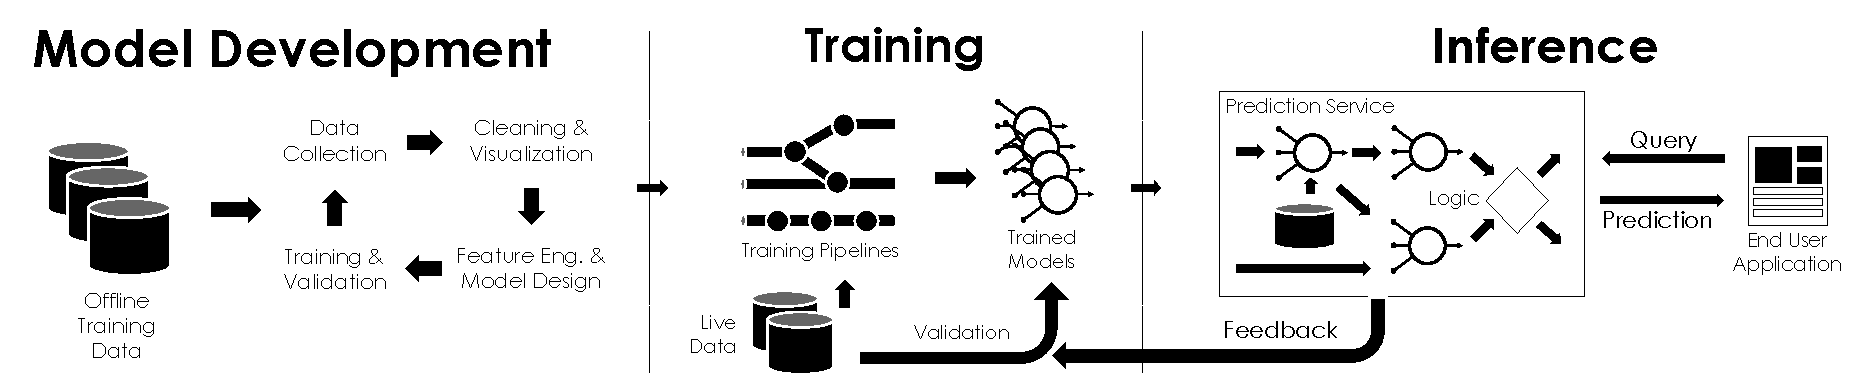
\includegraphics[width=\textwidth]{letters/pipeline.pdf}
\caption{\small \textbf{Machine Learning Life-cycle.} A simplified depiction of the key stages of a machine learning application.}
\label{fig:mllc}
\end{figure}


The machine learning life-cycle (Fig.~\ref{fig:mllc}) spans not only the model development, but also production training and inference.
Each stage demands different skills (e.g., neural network design, data management, and cluster management) and imposes different requirements on the underlying systems.
Yet there is an overwhelming need for unifying design principles and technologies to address pervasive problems including: feature management, data provenance, pipeline reproducibility, low-latency serving, and prediction monitoring just to name a few.


There has been substantial recent progress in systems to aid in managing the machine learning life-cycle.  
Large industrial projects like 
FB Learner Flow 
% \href{https://code.fb.com/core-data/introducing-fblearner-flow-facebook-s-ai-backbone/}{FB Learner Flow}
from Facebook, 
Michelangelo 
% \href{https://eng.uber.com/michelangelo/}{Michelangelo} 
from Uber, and 
TFX 
% \href{https://www.tensorflow.org/tfx/}{TFX} 
from Google have received a considerable of recent attention.  
In this issue we have solicited publications from several more recent industrial and academic projects.

The first paper, by a team at Amazon Research, provides an overview of several real-world use cases and then outlines the key conceptual, data management, and engineering challenges faced in production machine learning systems.
Rather than advocating a single system, this work describes some design principles that can inform potential solutions.


The second and third papers explores the challenges of model management and provenance across the machine learning life-cycle.
They motivate the need for systems to track models and their meta-data to improve reproducibility, collaboration, and governance. 
% expands upon the machine learning life-cycle 
% to include: data preparation, feature engineering, model training, deployment, and maintenance
% and explores the challenges of model 
The second paper introduces, ModelDB, an open-source system for model management and describe some of the functionality and design decisions. 
The third paper describes a related system, ProvDB, that uses a graph data model to capture and query fine-grained versioned lineage of data, scripts, and artifacts throughout the data analysis process.


The fourth paper, by a team at Databricks Inc., describes, MLFlow, a new open-source system to address the challenges of experimentation, reproducibility, and deployment. 
This work leverages containerization to capture the model development environment and a simple tracking API to enable experiment tracking.
The extensible model containerization enables model developers to more easily collaborate around modeling environments and then deploy model containers.


The last paper, by a team at Microsoft, focuses on inference and explores the challenges and opportunities of serving white-box prediction pipelines.  
In contrast to the containerization of pipelines in MLFlow, the Microsoft team leverage knowledge about the internal of the prediction pipeline to more efficient serve predictions. 



\end{document}




\end{letter}

\end{lettersection}

% put the name of your special issue below


\begin{opinionsection}
\begin{opinion}{A Wake-up Call: Managing Data in an Untrusted World}
{Divyakant Agrawal, Amr El Abbadi}{University of California, Santa Barbara}
\documentclass[11pt]{article}
%\usepackage[utf8]{inputenc}
\usepackage{url}

%\author{\\Department of Computer Science,
% University of California, Santa Barbara\\\textit{\{agrawal,}  \textit{amr\}@cs.ucsb.edu}}

\begin{document}
\title{A Wake-up Call: Managing Data in an Untrusted World}
\author{Divyakant Agrawal\qquad Amr El Abbadi\\
  University of California, Santa Barbara\\
  \textit{\{agrawal,}  \textit{amr\}@cs.ucsb.edu}}
%\maketitle
\vspace{1cm}

Once upon a time databases were structured, one size fitted all and they resided on machines that were trustworthy and even when they failed, they simply crashed.  This era has come and gone as eloquently stated by Stonebraker and Cetintemel~\cite{StonebrakerICDE2005}.  We now have key-value stores, graph databases, text databases, and a myriad of unstructured data repositories. The database community has wholeheartedly accepted the fact that the same information might come in different formats, modes and representations.  We also accept that data might not be "clean" and that data might need to be "cleaned" due to the diverse sources of information. However, we, as a database community still cling to our $20^{th}$ century belief that databases always reside on trustworthy, honest servers. Although the database community has always considered fault-tolerance as an integral building block of data management (remember "D" in ACID is for Durability), we still have trouble accepting the fact that not all failures are simply crash failures and might in fact involve malicious and non-trustworthy infrastructure. This notion has been challenged and abandoned by many other Computer Science communities, most notably the security and the distributed systems communities.  The rise of the cloud computing paradigm as well as the rapid popularity of blockchains demand a rethinking of our naïve, comfortable  beliefs in an ideal benign infrastructure.  In the cloud, clients store their sensitive data in remote servers owned and operated by cloud providers. The Security and Crypto Communities have made significant inroads to protect both data and access privacy from malicious untrusted storage providers using encryption and oblivious data stores.  The Distributed Systems and the Systems Communities have developed consensus protocols to ensure the fault-tolerant maintenance of data residing on untrusted, malicious infrastructure.  However, these solutions face significant scalability and performance challenges when incorporated in large scale data repositories. Novel database designs need to directly address the natural tension between performance, fault-tolerance and trustworthiness.  This is a perfect setting for the database community to lead and guide.  

In this opinion article, we will illustrate an interesting atomicity problem in the context of exchanging cryptocurrencies using permissionless blockchains. We also illustrate that transaction management can learn from the blockchain approach when attempting to restricted untrusted behaviour from the underlying infrastructure.  We hope this will illustrate some of the challanges that need to be addressed in malicious, untrusted settings, as well as connections with standard database problems like commitment, replication and transaction management in general. 

Bitcoin~\cite{nakamoto2008bitcoin} took the world by surprise over a decade ago by introducing a novel cryptocurrency, which supports the execution of transactions, albeit relatively simple transfers.  As with any data management system, bitcoin needed to address the challenge of durability.  Its approach, rather than using a trusted persistence storage device to store the current state, e.g., a disk, relies on global replication of a distributed data structure called a {\em blockchain}.  A blockchain is basically a linked list of blocks, each of them containing a set of transactions.  The blockchain is replicated on a potentially unknown number of {\em untrusted} servers.
Two of the main challenges that bitcoin needed to address are (1) the unknown number of participants and (2) the untrusted nature of the participants.  The former challenge basically manifests itself when consensus is needed to add a new block to the blockchain.  This is resolved by avoiding communication to achieve consensus, as is typical in Byzantine Agreement protocols, and replacing it with computation, namely the well-known {\em Proof of Work} mining puzzle operation.  The latter challenge is addressed using many different cryptographic techniques, including digital signatures, hash pointers, etc.  Currently, it seems that database vendors have adopted blockchains, with their untrusted infrastructure, but only in contexts where the number of untrusted participants is known {\em a priori}.  This problem is suitable for supply-chain, financial and healthcare applications. In blockchain terminology, this is referred to as {\em permissioned blockchains}.  Over the past few years different permissioned blockchain systems have been developed in both
industry and academia.
Some known industrial permissioned blockchain systems include Hyperledger Fabric \cite{androulaki2018hyperledger} which was introduced by IBM and is widely used in supply chain management,
Quorum \cite{morgan2016quorum} by JPMorgan which supports financial applications, and
Libra \cite{libra2019libra} is a digital currency by Facebook.
Similarly, in academia, Fast Fabric \cite{fastfabric2019}, ParBlockchain \cite{amiri2019parblockchain},
ResilientDB \cite{gupta2020resilientdb}, Caper \cite{amiri2019caper}, AHL \cite{dang2018towards}, etc. have been proposed. This is a good step, and demonstrates our willingness to address the challenges of untrusted as well as unreliable infrastructures.  However, we believe database researchers have a lot more to offer.  These efforts go in both directions, i.e., to extend support for untrusted infrastructures in diverse data management contexts, as well as exploiting data management techniques in diverse novel and non-traditional contexts, as for example in permissionless blockchains.


Bitcoin and other cryptocurrencies are {\em permissionless} blockchains.
In a permissionless blockchain, the network is public, and anyone can participate without a specific identity.
The recent adoption of blockchain technologies and open 
permissionless networks has demonstrated user needs to exchange assets
and especially without depending on centralized 
intermediaries such as banks or exchanges. 
This problem requires infrastructure enablers and protocols that allow users to 
{\em atomically} exchange assests without giving up trust-free decentralization,
the main reasons behind using  permissionless blockchain. We motivate the problem
of atomic cross-chain transactions and discuss
the current available solutions and their limitations through the following example.  

Suppose Alice owns X bitcoins and she wants to exchange them for Y 
ethers. Luckily, Bob owns ether and he is willing to exchange his Y ethers for X bitcoins. 
In this example, Alice and Bob want 
to atomically exchange assets that reside in different blockchains. In addition,
both Alice and Bob \textit{do not trust} each other and in many scenarios, 
they might not be co-located to do this atomic exchange in person.
Current infrastructures
do not support these direct peer-to-peer transactions. 
Instead, both Alice and Bob need to \textit{independently} exchange their 
assets through a trusted centralized exchange, Trent 
(e.g., Coinbase~\cite{coinbase} and Robinhood~\cite{robinhood}) either through
fiat currency or directly.  Using fiat, both Alice
and Bob first exchange their assets with Trent for a fiat currency (e.g., USD) and 
then use the earned fiat currency to buy the other assets also from Trent or from 
another trusted exchange. Alternatively, some exchanges (e.g., Coinbase) allow their 
customers to directly exchange assets (ether for bitcoin or bitcoin for ether) 
without going through fiat currencies.

A two-party cross-chain commitment protocol was originally proposed by 
Nolan~\cite{atomicNolan} and generalized by 
Herlihy~\cite{herlihy2018atomic} to process multi-party cross-chain transactions, or swaps.
Both Nolan's protocol and its generalization by Herlihy use smart contracts, hashlocks,
and timelocks to execute cross-chain transactions. A {\em smart contract} is a self executing
contract (or a program) that is executed in a blockchain 
once all the terms of the contract are satisfied. A {\em hashlock} is 
a cryptographic one-way hash function $h = H(s)$ that locks
assets in a smart contract until a hash secret $s$ is provided. A {\em timelock} is a time 
bounded lock that triggers the execution of a smart contract function
after a pre-specified time period. 
%It is interesting to note how many of these basic tools are quite familiar to database practitioners.
These proposals solve the cross-chain commitment problem and ensure that untrusted participants comply and do not try to misuse the system.
However, an expired timelock could lead to a violation of the all-or-nothing
atomicity property. An honest participant who fails to react in time due to a crash failure, network delays or even a denial of service attack 
might end up losing their assets. Although a crashed participant
is the only participant who ends up worse off, current proposals are
unsuitable for atomic cross-chain transactions in asynchronous 
environments where crash failures and network delays are the norm. 
This is a problem familiar to the database community since its inception, namely the {\em atomic commitment problem}.  In~\cite{zakhary2020atomic}, we present a decentralized all-or-nothing \textit{atomic} cross-chain commitment protocol.  Events for redeeming and refunding smart contracts to exchange assets are 
modeled as conflicting events. An open permissionless network of witnesses is 
used to guarantee that conflicting events could never simultaneously occur 
and either all smart contracts in an atomic cross-chain transaction
are redeemed or all of them are refunded.  A similar protocol was also concurrently proposed by Herlihy et al.~\cite{Herlihy2020VLDB}, which addresses the same atomicity challenge, but in the context of {\em cross chain deals}, where a {\em deal} is a weaker notion of an atomic transaction.

Now, we briefly come back to traditional databases and large scale data fault-tolerant transaction management but on untrusted infrastructures.  As increasing amounts of data are currently being stored and managed on third-party servers, there is emerging demand for a suite of protocols to manage data on untrusted infrastructures. In Fides~\cite{maiyya2020fides}, we introduce a novel atomic commitment protocol, TFCommit, that executes transactions on data stored across multiple untrusted servers. This novel atomic commitment protocol executes transactions in an untrusted environment without the need for expensive Byzantine replication. One main obstacle for the adoption of Byzantine Agreement protocols are the various impossibility results, that require {\em a priori} knowledge of the maximum possible number of failures in the system (e.g., one third in case of malicious failures).  From a practical point of view, this might be difficult to ascertain.  We propose using TFCommit in an {\em auditable} data management system, Fides, residing completely on untrustworthy infrastructures. As an auditable system, Fides guarantees the detection of potentially malicious failures occurring on untrusted servers using blockchain inspired tamper-resistant logs with the support of cryptographic techniques. As a result, Fides is scalable and does not require any {\em a priori} known bounds on the number of malicious faults when executing transactions on untrusted infrastructure.  If malicious behaviour occurs, it is recorded and can be detected by an external auditor.  Just the threat of investigation should usually deter improper behaviour.

In conclusion, we encourage researchers to explore a relatively new and uncharted domain for the database community.  Many techniques have indeed been developed by the security, cryptography and distributed systems communities.  However, these solutions are often too expensive to use in the practical scalable settings data management systems encounter on a daily basis. 
In fact, we view this as a two way exchange of ideas and innovations.  Over four decades of fault-tolerant data management innovations can be beneficial and can have significant impact in solving many of the practical large scale problems that need to be addressed in untrusted infrastructures.   On the other hand, many of the techniques developed to restrict malicious behaviour using cryptographic and distributed computing approaches can facilitate the development of fault-tolerant database management systems in untrused infrastructures, which are becoming more prevalent and commonplace for storing data.
\section*{Acknowledgement}

This work is partially funded by NSF grants CNS-1703560 and CNS-1815733.

\begin{thebibliography}{10}

\bibitem{coinbase}
Coinbase.
\newblock \url{https://coinbase.com}, 2018.

\bibitem{robinhood}
Robinhood.
\newblock \url{https://robinhood.com/}, 2018.

\bibitem{amiri2019caper}
Mohammad~Javad Amiri, Divyakant Agrawal, and Amr~El Abbadi.
\newblock Caper: a cross-application permissioned blockchain.
\newblock {\em Proceedings of the VLDB Endowment}, 12(11):1385--1398, 2019.

\bibitem{amiri2019parblockchain}
Mohammad~Javad Amiri, Divyakant Agrawal, and Amr~El Abbadi.
\newblock Parblockchain: Leveraging transaction parallelism in permissioned
  blockchain systems.
\newblock In {\em 39th International Conference on Distributed Computing
  Systems (ICDCS)}, pages 1337--1347. IEEE, 2019.

\bibitem{androulaki2018hyperledger}
Elli Androulaki, Artem Barger, Vita Bortnikov, Christian Cachin, et~al.
\newblock Hyperledger fabric: a distributed operating system for permissioned
  blockchains.
\newblock In {\em EuroSys Conference}, page~30. ACM, 2018.

\bibitem{morgan2016quorum}
JP~Morgan Chase.
\newblock Quorum white paper, 2016.

\bibitem{dang2018towards}
Hung Dang, Tien Tuan~Anh Dinh, Dumitrel Loghin, Ee-Chien Chang, Qian Lin, and
  Beng~Chin Ooi.
\newblock Towards scaling blockchain systems via sharding.
\newblock In {\em Proceedings of the 2019 ACM SIGMOD International Conference
  on Management of Data}. ACM, 2019.

\bibitem{fastfabric2019}
Christian Gorenflo, Stephen Lee, Lukasz Golab, and S.~Keshav.
\newblock Fastfabric: Scaling hyperledger fabric to 20,000 transactions per
  second.
\newblock {\em arXiv preprint arXiv:1901.00910}, 2019.

\bibitem{gupta2020resilientdb}
Suyash Gupta, Sajjad Rahnama, Jelle Hellings, and Mohammad Sadoghi.
\newblock Resilientdb: Global scale resilient blockchain fabric.
\newblock {\em arXiv preprint arXiv:2002.00160}, 2020.

\bibitem{herlihy2018atomic}
Maurice Herlihy.
\newblock Atomic cross-chain swaps.
\newblock In {\em ACM Symposium on Principles of Distributed Computing (PODC)},
  pages 245--254. ACM, 2018.

\bibitem{Herlihy2020VLDB}
Maurice Herlihy, Liuba Shrira, and Barbara Liskov.
\newblock Cross-chain deals and adversarial commerce.
\newblock {\em Proc. {VLDB} Endow.}, 13(2):100--113, 2019.

\bibitem{maiyya2020fides}
Sujaya Maiyya, Danny Hyun~Bum Cho, Divyakant Agrawal, and Amr~El Abbadi.
\newblock Fides: Managing data on untrusted infrastructure.
\newblock {\em arXiv preprint arXiv:2001.06933}, 2020.

\bibitem{libra2019libra}
Libra~Association Members.
\newblock An introduction to libra.
\newblock {\em https://libra.org/en-US/white-paper/}, 2020.

\bibitem{nakamoto2008bitcoin}
Satoshi Nakamoto.
\newblock Bitcoin: A peer-to-peer electronic cash system.
\newblock 2008.

\bibitem{atomicNolan}
Tier Nolan.
\newblock Alt chains and atomic transfers.
\newblock
  \url{https://bitcointalk.org/index.php?topic=193281.msg2224949#msg2224949},
  2013.

\bibitem{StonebrakerICDE2005}
Michael Stonebraker and Ugur {\c{C}}etintemel.
\newblock "one size fits all": An idea whose time has come and gone (abstract).
\newblock In Karl Aberer, Michael~J. Franklin, and Shojiro Nishio, editors,
  {\em Proceedings of the 21st International Conference on Data Engineering,
  {ICDE} 2005, 5-8 April 2005, Tokyo, Japan}, pages 2--11. {IEEE} Computer
  Society, 2005.

\bibitem{zakhary2020atomic}
Victor Zakhary, Divyakant Agrawal, and Amr El~Abbadi.
\newblock Atomic commitment across blockchains.
\newblock {\em Proceedings of the VLDB Endowment}, 13:1, 2020.

\end{thebibliography}
\end{document}

\end{opinion}
\begin{opinion}{The Battle for Data Science}
{Jeffrey D. Ullman}{Stanford University}
\documentclass[11pt]{article} 
\usepackage{deauthor,times,graphicx}%,hyperref} 

\begin{document}
\title{The Battle for Data Science}
\author{Jeffrey D. Ullman\\Stanford University, Dept.\ of Computer Science\\ullman@gmail.com}

%\maketitle

\section{Introduction}

Through the years, the database community has periodically looked at developments in technology and engaged in hand-wringing over the idea that we are becoming irrelevant.  The cry ``have we missed the boat~-- again'' is common; e.g., here is a panel I served on several years ago \cite{boat}.
My goal in this essay is to argue that the database field and the techniques that have come from this research are still essential for ``data science,'' that is, for the exploitation of data to solve problems of importance in application fields~-- science, commerce, medicine and such.  I believe, as I assume most readers of this article believe, that the field of database systems has always had at its core the study of how to deal with the largest amounts of data possible at the time, whether that be megabytes of corporate payroll data, terabytes of genomic information, or petabytes of satellite output.  Thus whatever study of data is necessary at the time~-- that's our job.

To advance this argument, I want to look at three issues:

\begin{enumerate}

\item
Is the field of statistics really the essential ingredient in data science?

\item
Is machine learning really what data science is all about?

\item
Is data science a danger to decent societal norms?

\end{enumerate}
Hint: my answer to all three is ``no.''  I'll try to address each of these in turn.

\section{The Battle Line: Venn Diagrams for Data Science}

Several years ago, I was invited to a panel of the National Research Council called the ``Data-Science-Education Roundtable.''  The output of this group can be seen at \cite{dsr}.  It was organized not by the computer-science wing of the NRC but the statistics branch.  The participants were roughly equally divided between  statisticians and computer scientists, plus a few from other disciplines.  Part of my experience was seeing how statisticians thought about the world of data and its application.  The most obvious point was that the field of statistics views data science as its own.

To be fair, let's be clear at the outset that I have great respect for statisticians and the work they do.
Statistics has become increasingly important to the modern study of data, including, but not limited to machine learning.
Many statisticians are starting to focus on computation and data analysis in the same way as we do in the database community or in
computer science more generally.  Just to offer one small example, one of my favorite techniques is locality-sensitive hashing, which is an
idea that came squarely out of the database community \cite{lsh}.   Yet one of my colleagues in the Statistics Department at Stanford, Art Owen,
showed me something \cite{owen} about a key step, minhashing \cite{minhash}, that speeds up the process by a very large factor -- something we should have been able to figure out years ago, but didn't.

However, my experience in the roundtable also gave me the sense that there is an effort on the part of some in the statistics community to define statistics as the central component of data science.  I, in contrast, would see the algorithms and techniques for processing large-scale data efficiently as the center of data science.  There is a general sense that data science is a discipline that combines the knowledge of several fields, and I agreed completely.  But what are those fields, and how do they interact?  The question is considered so important that competing communities have published Venn diagrams to justify their own centrality in data science.  There was a recent article \cite{venn} summarizing and commenting upon  a number of these diagrams.  Or if you really want to see the full spectrum of viewpoints expressed as venn diagrams, issue the search query [wikipedia data science venn diagrams].

\subsection{The Conway Diagram}

It appears that statisticians all use a particular diagram, due to Drew Conway.  This diagram shows three sets intersecting: ``hacking skills,'' ``math and statistics,'' and ``substantive expertise.''  At the roundtable, this diagram was shown several times to illustrate the importance of statistics, and I have seen statisticians in several other contexts showing the same diagram to explain the importance of their field to data science.  I reproduce the diagram in Fig.~\ref{drew-diagram-fig}, but I have added my own edits and comments to explain what is misleading about the diagram.

\begin{figure}[h]
\centerline{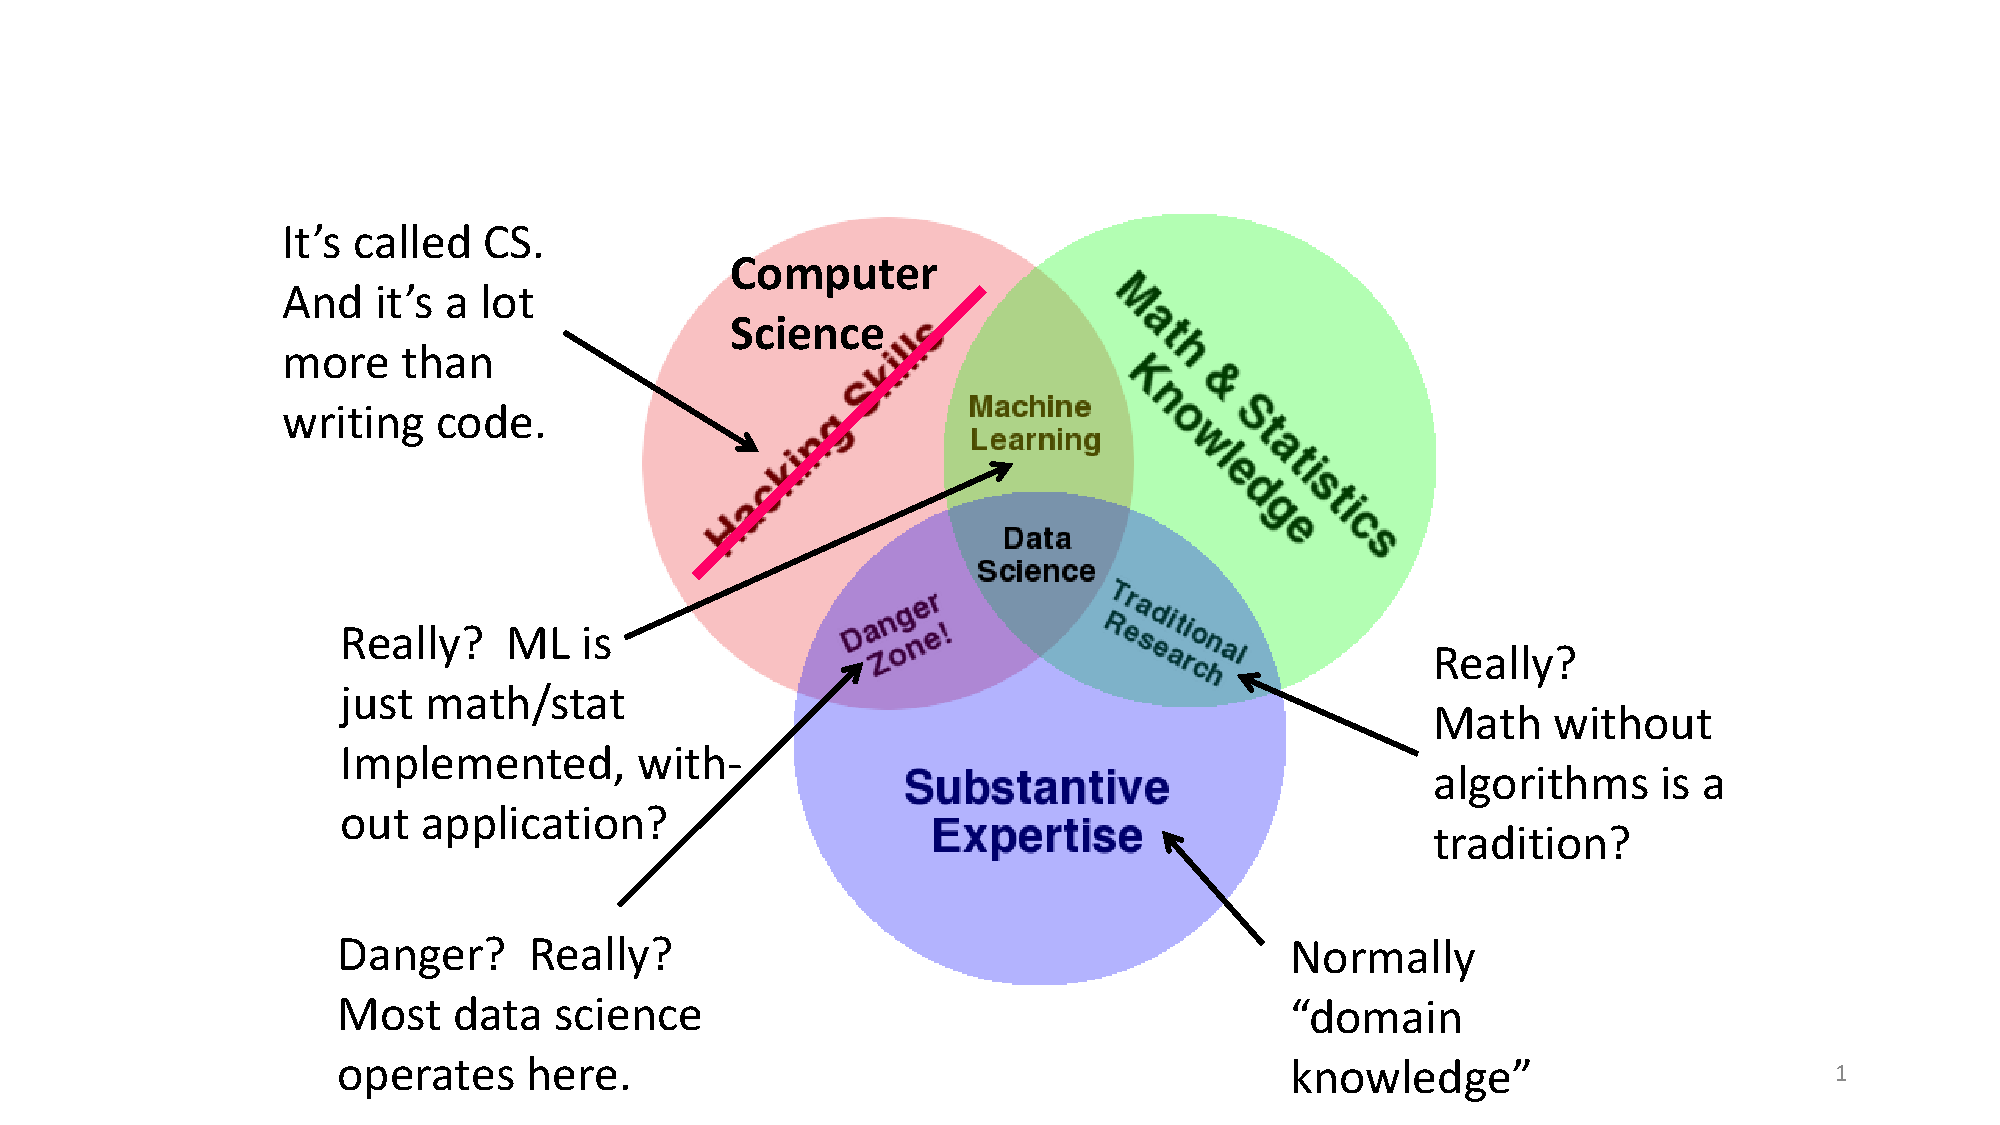
\includegraphics[width=0.8\textwidth]{letters/drew-diagram.pdf}}
\caption{The Conway Venn diagram for data science}
\label{drew-diagram-fig}
\end{figure}

In fact, almost every region of the diagram is misleading in some way.

\begin{enumerate}

\item
First, a small matter: what is referred to as ``substantive expertise'' is generally called ``domain knowledge'' or something similar.

\item
The most egregious impropriety is referring to computer science as ``hacking skills.''  Computer science brings far more to data science than the ability to write code.  We offer algorithms, models, and frameworks, for solving problems of all sorts.  All of that is essential in dealing with data.

\item
``Traditional research'' is shown in the diagram as math/stat intersected with applications.  In other words, in this form of research, one thinks about the application, but does not write any code, and therefore there is nothing that affects the real world.  I don't know whose tradition that is, but I am glad to say it is not the tradition of the database community.

\item
Machine learning has an odd place in this diagram.  It is described as ``hacking'' plus math/stat.  The implication is that machine learning has nothing to do with applications.  In practice, it has everything to do with applications, which is why today the algorithms from machine learning are taken so seriously, not only in the database community, but all across computer science.

\item
And then there is what Conway calls the ``danger zone''~-- writing code to solve problems in application areas without the wise guidance of a statistician.  Well almost all of data science is like that.  For just one example, Google and other mail services are pretty good at detecting phishing emails.  How good?  We really don't know, and even if we could do a statistical analysis today, it would not be valid tomorrow, as the threats change.  The real danger would be refusing to do the best we could, and letting some poor soul send their life savings to some scam artist.

\end{enumerate}

\subsection{My Venn Diagram}

I too offered a Venn diagram (Fig. \ref{myvenn-fig}) that I believe better represents the relationships between the fields.  There is computer science and the various domain sciences, and somewhere in the intersection of these is data science.  Machine learning is a branch of computer science~-- a very important subset these days.  Some of machine learning is used for data science, although there are other uses of machine learning that are more internal to computing.  Many of these applications are considered ``artificial intelligence'' these days, e.g., driverless cars or intrusion detection.  Finally, I see both math and statistics as very important tools for all of computer science, and the small bubbles in my diagram do not do justice to their importance.  However, I drew them as shown to emphasize that they do not really impact domain sciences directly.  but rather they do so through the software that is developed, often with their important aid.

\begin{figure}[h]
\centerline{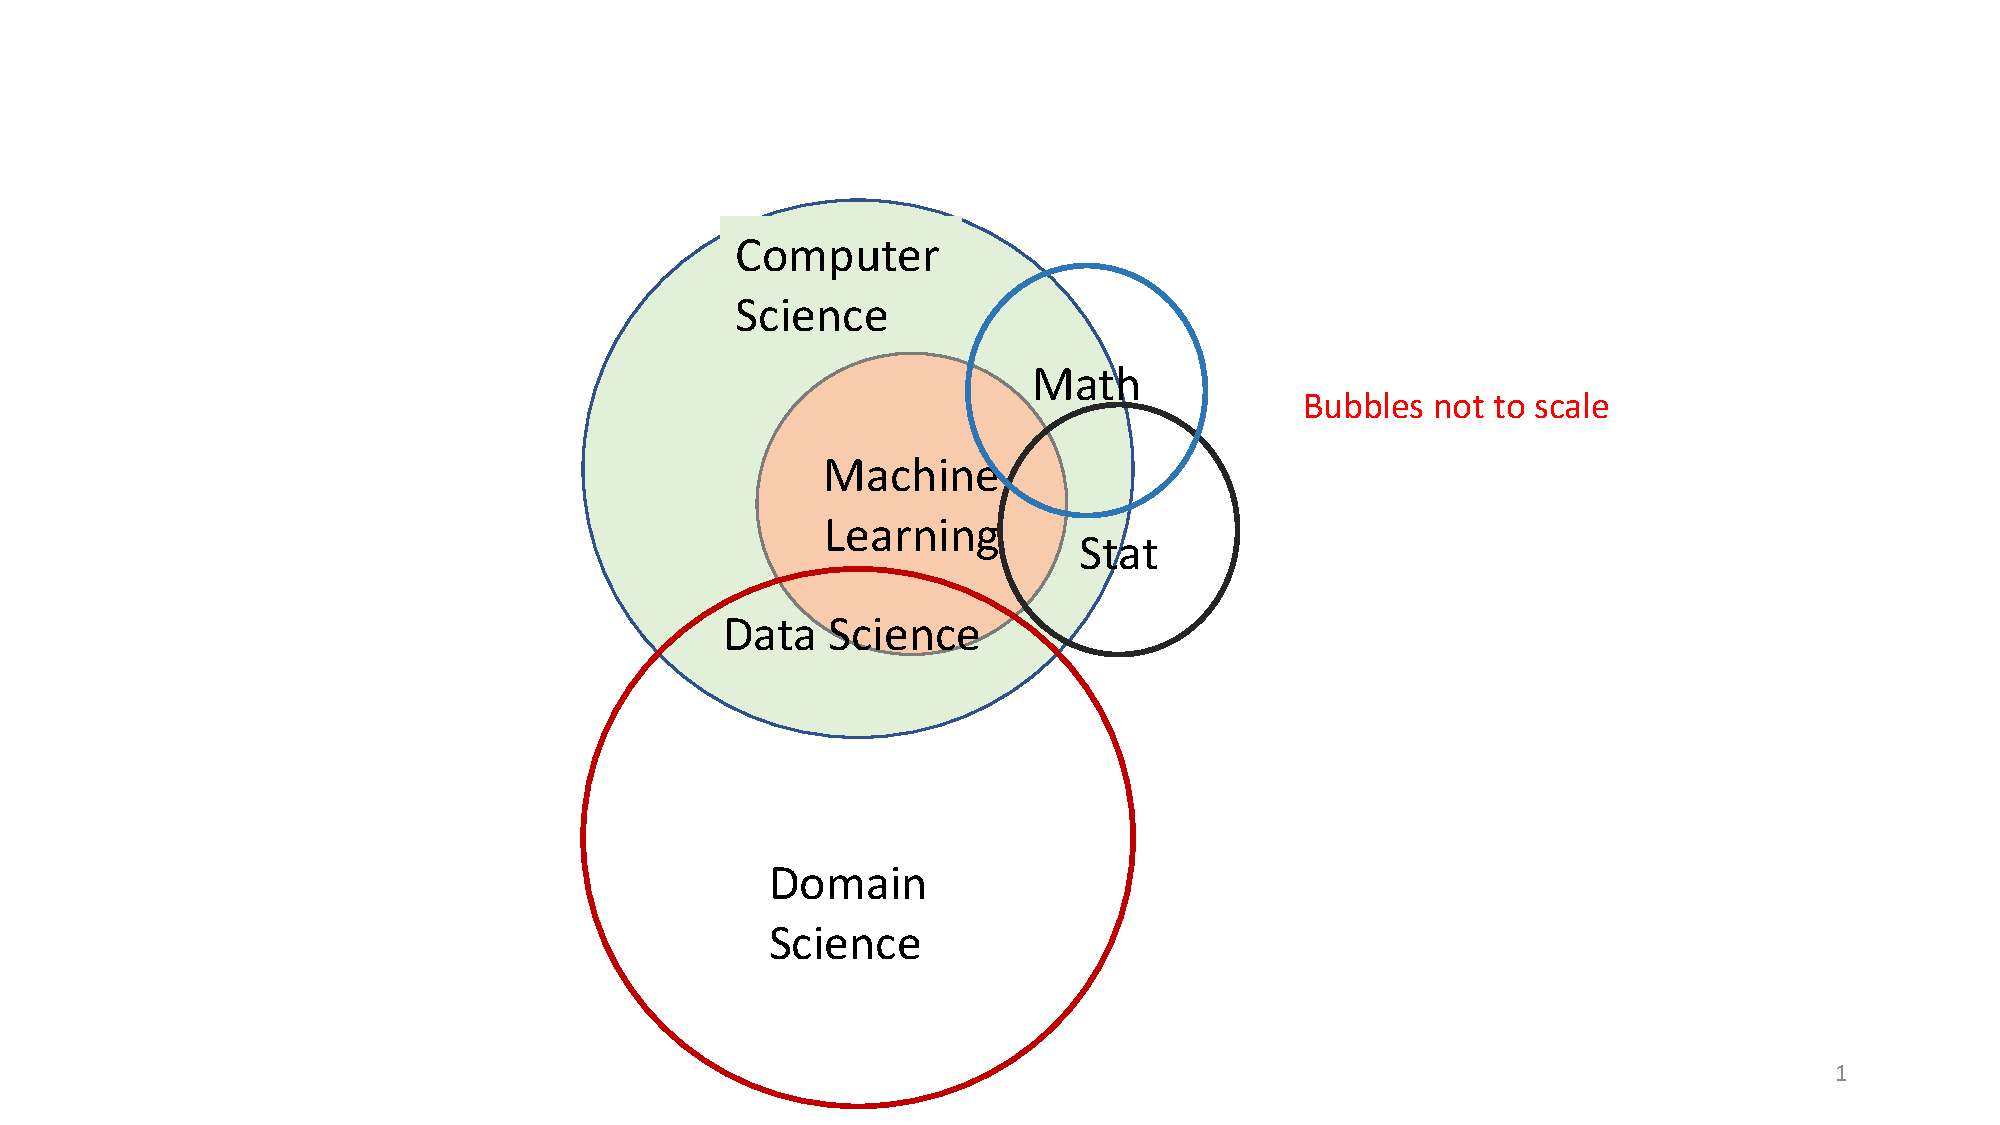
\includegraphics[width=0.8\textwidth]{letters/myvenn.pdf}}
\caption{A personal view of the relationship between computer science, machine learning, and statistics}
\label{myvenn-fig}
\end{figure}

\subsection{The Big Difference: Database and Statistics Value Systems}

Perhaps the most contentious implication of my diagram is that math/stat does not address domain applications directly.  After all, the Conway diagram talks about ``traditional research'' as doing just that.  But while there may be interaction between applications and math/stat that bypasses computing, I think it is rare that the interaction results in any benefit to the application.

To illustrate the distinction, look at the report of the fourth meeting of the data-science education roundtable \cite{datafest}.  One part of the discussion centered on the ``hackathon'' run by the American Statistical Association, called ``Datafest.''  Superficially, this event is just like the sort of hackathon we see run for computer-science students.  The competing teams are given a large dataset, drawn from some application area.  But there is a big difference in how the competition is evaluated.  Competitors are not expected to solve someone's problem, and are not evaluated on the quality of their solution.  Rather, ``awards were given for best data visualization, best use of external data, and best insight.''  In other words, you win a statistical hackathon by doing something of interest to statisticians, not by solving someone else's problem.  I hope the reader appreciates the opposite approach, where the goal is to serve, not to amuse oneself.  That approach, for example, is what drives the computer-science-oriented Kaggle competitions \cite{kaggle}.

\section{Database Systems and Machine Learning}

Now, let us turn to how the rise of machine learning has impacted the use of data.  There is no question that machine learning has had enormous impact on our ability to use data to solve problems.  Many of the most impressive recent achievements have been applications of algorithms in the machine-learning class.  However, I do not believe that machine learning is a complete replacement for the algorithms that have been developed in the database community.  I wish the reader to consider three issues:

\begin{enumerate}

\item
There are many problems involving ``big data'' that are not really machine-learning problems.

\item
Not everything that machine learning claims as its own really comes from there.

\item
Many machine-learning methods produce mysterious models that do not support explanation or justification.

\end{enumerate}

\subsection{Machine Learning Is Not All of Data Science}

I believe a fair definition of machine learning is algorithms that use data to create a model of something, from which answers can be derived.  For example, machine learning can be used to build a model of spam emails, so that a given email can be fed to the model and reliably found to be spam or not spam (``ham'').  But not every useful solution can be expressed as a model.  For example, we earlier mentioned locality-sensitive hashing (LSH) as an important technique from the database community for dealing with data.  LSH is a body of techniques (see, e.g., Chapter 3 of \cite{mmds}) for finding similar items in a dataset without having to look at all pairs.  You don't need for the dataset to be very large before looking at all pairs is prohibitive; even a million items in your set implies half a trillion pairs that would need to be looked at.  So when applicable, LSH can be a very powerful tool.  But there is no model involved.  It is not an instance of machine learning.

\subsection{Machine-Learning Advocates Sometimes Claim Too Much}

I have heard of clustering, for example, defined as a branch of machine learning, even though clustering has been studied from well before there was such a thing as machine learning.  Gradient descent is another example of something that predates machine learning, yet somehow is popularly regarded as a machine-learning topic.  Another important example concerns {\em association rules}.  This idea was pioneered in 1993--4 by Rakesh Agrawal and his friends \cite{ais} \cite{as} and predates almost all of machine learning.   I even recall talking to a machine-learning advocate and offering LSH as an example of a big-data algorithm that had nothing to do with machine learning.  His response was that LSH ``must be machine learning, because it is a really good idea.''

\subsection{Explainability}

Often, a machine-learning algorithm draws correct conclusions that cannot be explained except by showing the model.  And that model is often so complex that it means nothing to the average user.  Sometimes, no one cares; the important thing is that the model, say, gives the correct diagnosis, even if its reasoning is hidden in the processing of a megapixel image.  On the other hand, sometimes, we have a right to an explanation.  For example, if your insurance company raises your rates because some model of automobile accidents has decided you are more likely to have an accident than the previous model showed, it seems proper that you at least be told why this is happening to you.  In Europe, the GDPR laws \cite{gdpr} guarantee you that right.

But non-machine-learning approaches are often more explainable than machine-learning models.  To see the difference, let us reconsider the matter of association rules as a way to identify spam emails.  One would produce a set of ``rules,'' which in this case would be sets of words, whose presence in an email indicates it is spam.  You might think of these rules as a model of spam, which is probably why machine-learning advocates view the method as their own.  But in fact, the algorithms used to find association rules do not ``learn'' a model from the data.  They simply count the number of spam emails that contain certain sets of words, and if that count is high enough, they declare a rule that emails containing that set of words is spam.  For instance, we might expect that one rule would say that emails containing the set $\{${\tt Nigerian}, {\tt prince}$\}$ are spam.  In contrast, even the simplest machine-learning technique, such as learning a (positive or negative) weight on each possible word, and declaring spam if the sum of the weights exceeds a threshold, will be more accurate than a solution based on association rules.

However, the association-rule approach is explainable, while the machine-learning model is not.  If I really {\em am} a Nigerian prince, and all my emails are sent to spam, at least I can understand why.  On the other hand, if you have ever asked gmail why it declared something to be spam, its usual answer is something like ``it looked like other emails that were spam.''  That is, whatever model we are using today said it was spam, and that's all we can tell you.\footnote{Interestingly, I was the victim in way similar to that of the hypothetical Nigerian prince.  A dean asked me for a letter concerning a candidate for promotion, which I sent.  He claimed the email never arrived, so I sent it again.  It never arrived.  Eventually, he discovered that the mail system at his university had a rule that said anything from my email address was to be discarded immediately.  I suspect someone at some time engaged in a denial-of-service attack using my faked email address.  At least we were able to understand the problem and get it fixed quickly.}

\section{Attacks on the Use of Data}

It is common to blame data for the ills of society.  However, the fault rarely lies in the idea of using data to address a social issue.  Rather, the source of error is more likely to come from:

\begin{enumerate}

\item
People intentionally or unintentionally misusing the data, or

\item
Problems in the reality that the data faithfully reflects.

\end{enumerate}

\subsection{Misuse of Data}

At the Data-Science-Education Roundtable, there was a discussion in the fifth session on data ethics, which you may find in \cite{ethics}.  One common problem discussed was the use of ``false proxies.''  For an example given there, a city wants to deploy its police to the areas where crime occurs.  What they have is data on where arrests occur, so they send their police there, and lo and behold, they arrest more from those areas.  But arrests do not reflect solely the occurrence of crime; they also reflect the presence of police to make the arrests.  So a possible error is perpetuated by the data.  That is, if for bad reasons, police had been sent to certain areas preferentially in the past, the data will truly reflect that there are more arrests in those areas.  Perhaps, just as much crime occurs elsewhere, but the arrest rate is lower in places where the police presence is low.

Another common example of where data can perpetuate bias concerns a hypothetical company that has always discriminated against women when promotions are handed out.  They want to build an AI system using machine learning, to process resumes and identify those with characteristics similar to those of their successful employees.  But the data shows that being female is an indication that the candidate will not be successful, so the machine-learning algorithm learns from the data to reject applications from females.   The data again perpetuates an existing bias.  But the data didn't create the bias; people did.

\subsection{Data Reflecting a World We Don't Like}

A less reasonable charge against the use of data is that the resulting systems reflect something about society that the speaker opposes.  A clear example of this sort of false reasoning concerns Word2Vec \cite{word2vec}, a system developed at Google several years ago (since popularly superseded by an alternative system called BERT \cite{bert}) that embeds words in a high-dimensional vector space, in such a way that words with similar meaning have vectors that are close.  The intuitive idea is to look at the words that typically surround the word $w$ in question.  The vector for $w$ then is a weighed combination of directions associated with its surrounding words.  For example, we would expect {\tt Coke} and {\tt Pepsi} to have similar vectors, because people talk about them in much the same way.

The problem arose when it was observed that certain vector equations were approximately followed.  For example, as vectors,

\begin{center}
{\tt London} $-$ {\tt England} + {\tt France} = {\tt Paris}
\end{center}
That is, London and Paris, being the capitals and largest cities of their respective countries, have around them many words reflecting that status.  However, we would expect London to have more words that are associated with England surrounding it, so take them away and substitute words associated with France.

No one was disturbed by that observation, but other equations raised some hackles.  For instance, \cite{buono} called out the equation

\begin{center}
{\tt doctor} $-$ {\tt man} + {\tt woman} = {\tt nurse}
\end{center}
A similar objection to another such equation is discussed in \cite{boluk}.  However, if you look at this equation, it is asking ``find me a profession like doctor, but with more females.  About 50\% of doctors are women, but close to 90\% of nurses are women.  We expect that words surrounding {\tt doctor} and {\tt nurse} would be similar, but the latter will more often be found near words like {\tt she}.  So the equation makes sense.  What these negative articles are really objecting to is a society where women are more likely to be channeled into nursing.  I agree, and probably in the not-too-distant future, that will not be the case.  But my point is: don't blame the data.  Systems like Word2Vec or BERT, when trained on a large corpus like Wikipedia, will reflect language as used by a broad segment of the public, and that usage will in turn reflect what is generally thought to be true, regardless of whether we like that truth or not.

\section{The Last Word}

I hope the reader will take away the following thoughts:

\begin{itemize}

\item
Data and its management is still the essence of data science.

\item
While machine learning is very important, it is far from the only tool or idea needed for effective data science.

\item
Although there have been misuses of data, we should not blame data if it reflects the world as it is, rather than as we would like it to be.

\end{itemize}

\vspace{-.1cm}
\bibliographystyle{ACM-Reference-Format}
\begin{thebibliography}{10}
\begin{small}
\itemsep=-.5pt

\bibitem{ais}
R. Agrawal, T. Imielinski, and A. Swami,
``Mining associations between sets of items in massive databases,''
{\em Proc.\ ACM SIGMOD Intl.\ Conf.\ on Management of Data},
pp.~207--216, 1993.

\bibitem{as}
R. Agrawal and R. Srikant,
``Fast algorithms for mining association rules,''
{\em Intl.\ Conf.\ on Very Large Databases}, pp.~487--499, 1994.

\bibitem{boluk}
T. Bolukbasi, K.-W. Chang, J. Zou, V. Saligrama, and A. Kalai,
``Man is to computer programmer as woman is to homemaker? Debiasing word embeddings,''
{\em 30th Conference on Neural Information Processing Systems}, Barcelona, 2016.

\bibitem{minhash}
A.Z. Broder, M. Charikar, A.M. Frieze, and M. Mitzenmacher,
``Min-wise independent permutations,''
{\em ACM Symposium on Theory of Computing}, pp.~327--336, 1998.

\bibitem{buono}
T. Buonocore, ``Man is to doctor as woman is to nurse: the gender bias of word embeddings,'' https://towardsdatascience.com/gender-bias-word-embeddings-76d9806a0e17

\bibitem{bert}
J. Devlin, M.-W. Chang, K. Lee, and K. Toutanova,
``BERT: Pre-training of deep bidirectional transformers for language understanding,''
arXiv:1810.04805, 2018.

\bibitem{lsh}
A. Gionis, P. Indyk, and R. Motwani,
``Similarity search in high dimensions via hashing,''
{\em Proc.\ Intl.\ Conf.\ on Very Large Databases}, pp.~518--529, 1999.

\bibitem{boat}
B. Howe, M.J. Franklin, L.M. Haas, T. Kraska, and J.D. Ullman:
``Data science education: we're missing the boat, again,'' {\em ICDE}, pp.~1473--1474, 2017.

\bibitem{kaggle}
https://www.kaggle.com/

\bibitem{venn}
https://www.kdnuggets.com/2016/10/battle-data-science-venn-diagrams.html

\bibitem{mmds}
J. Leskovec, A. Rajaraman, and J.D.Ullman,
{\em Mining of Massive Datasets} 3rd edition, Cambridge Univ.\ Press, 2020.  Available for download at http://www.mmds.org

\bibitem{owen}
P. Li, A.B. Owen, and C.H. Zhang.
``One permutation hashing,''
{\em Conf.\ on Neural Information Processing Systems} 2012, pp.~3122--3130.

\bibitem{word2vec}
T. Mikolov, K. Chen, G. Corrado, and J. Dean,
``Efficient estimation of word representations in vector space,''
ArXiv:1301.3781, 2013.

\bibitem{datafest}
https://www.nationalacademies.org/event/10-20-2017/docs/DCE05D1E271C31C585455B25E43AE9E5462ED3312DB2

\bibitem{ethics}
https://www.nationalacademies.org/event/12-08-2017/docs/D8EE65EFC7F4B0C368D267EDAD10E5AB1BAFBE3369D2

\bibitem{dsr}
https://www.nationalacademies.org/our-work/roundtable-on-data-science-postsecondary-education

\bibitem{gdpr}
https://en.wikipedia.org/wiki/Right\_to\_explanation


\end{small}
\end{thebibliography}

\end{document}

\end{opinion}
\end{opinionsection}

\begin{articlesection}{Data Technologies Behind Digital Contact Tracing for COVID19}
%
%  Contributed articles section.  Use the articlesection environment.
%  Each article is contained in an article environment, where the two required
%  options to \begin{article} are the title and author of the article
%
%\begin{article}
%{Title of article}
%{list of authors}
%\input{author-name/article.tex}
%\end{article}




\makeatletter
\renewcommand{\AB@affillist}{}
\renewcommand{\AB@authlist}{}
\setcounter{authors}{0}
\makeatother

\begin{article}
{{PACT\/}:   {P\/}rivacy-Sensitive Protocols { A\/}nd Mechanisms for Mobile {C\/}ontact { T\/}racing}
{Justin Chan, Dean Foster, Shyam Gollakota, Eric Horvitz,  Joseph Jaeger, Sham Kakade, Tadayoshi Kohno, 
John Langford, Jonathan Larson, Puneet Sharma, Sudheesh Singanamalla,
Jacob Sunshine, Stefano Tessaro}
\graphicspath{{submissions/pact/}}
\subimport{submissions/pact/}{main.tex}
\end{article}


\makeatletter
\renewcommand{\AB@affillist}{}
\renewcommand{\AB@authlist}{}
\setcounter{authors}{0}
\makeatother

\begin{article}
{Decentralized Privacy-Preserving Proximity Tracing}
{Carmela Troncoso, 
Mathias Payer, 
Jean-Pierre Hubaux, 
Marcel Salath\'e, 
James Larus, 
Wouter Lueks, 
Theresa Stadler,
Apostolos Pyrgelis,
Daniele Antonioli,
Ludovic Barman,
Sylvain Chatel,
Kenneth Paterson,
Srdjan Capkun, 
David Basin,
Jan Beutel,
Dennis Jackson,
Marc Roeschlin,
Patrick Leu,
Bart Preneel,
Nigel Smart,
Aysajan Abidin,
Seda G\"urses,
Michael Veale,
Cas Cremers,
Michael Backes,
Nils Ole Tippenhauer,
Reuben Binns,
Ciro Cattuto,
Alain Barrat,
Dario Fiore,
Manuel Barbosa,
Rui Oliveira,
Jos\'e Pereira}
\graphicspath{{submissions/dp3t/}}
\subimport{submissions/dp3t/}{DP3T.tex}
\end{article}


\makeatletter
\renewcommand{\AB@affillist}{}
\renewcommand{\AB@authlist}{}
\setcounter{authors}{0}
\makeatother


\begin{article}
{Contact Tracing: Holistic Solution Beyond Bluetooth}
{Ramesh Raskar, Deepti Pahwa, Robson Beaudry }
\graphicspath{{submissions/safepaths/}}
\subimport{submissions/safepaths/}{safepaths.tex}
\end{article}


\makeatletter
\renewcommand{\AB@affillist}{}
\renewcommand{\AB@authlist}{}
\setcounter{authors}{0}
\makeatother

\begin{article}
{Slowing the Spread of Infectious Diseases Using Crowdsourced Data}
{Sydney Von Arx, Isaiah Becker-Mayer, Daniel Blank, Jesse Colligan, Rhys Fenwick, Mike Hittle, Mark Ingle, Oliver Nash, Victoria Nguyen, James Petrie, Jeff Schwaber, Zsombor Szabo, Akhil Veeraghanta, Mikhail Voloshin, Tina White, and Helen Xue}
% \def\input@path{{{submissions/BerkeleyCovista/}{submissions/BerkeleyCovista/}}}
\graphicspath{{submissions/covidwatch/}}
\subimport{submissions/covidwatch/}{covidwatch.tex}
\end{article}


\makeatletter
\renewcommand{\AB@affillist}{}
\renewcommand{\AB@authlist}{}
\setcounter{authors}{0}
\makeatother

\begin{article}
{CoVista: A Unified View on Privacy Sensitive Mobile Contact Tracing}
{David Culler, Prabal Dutta, Gabe Fierro, Joseph E. Gonzalez, Nathan Pemberton, Johann Schleier-Smith, K. Shankari, Alvin Wan, and Thomas Zachariah}
% \def\input@path{{{submissions/BerkeleyCovista/}{submissions/BerkeleyCovista/}}}
\graphicspath{{submissions/BerkeleyCovista/figs/}}
\subimport{submissions/BerkeleyCovista/}{ms.tex}
\end{article}


\makeatletter
\renewcommand{\AB@affillist}{}
\renewcommand{\AB@authlist}{}
\setcounter{authors}{0}
\makeatother

\begin{article}
{Epione: Lightweight  Contact Tracing with Strong Privacy}
{Ni Trieu, Kareem Shehata, Prateek Saxena, Reza shokri, and Dawn Song}
% \def\input@path{{{submissions/BerkeleyCovista/}{submissions/BerkeleyCovista/}}}
\graphicspath{{submissions/Epione/figs/}}
\subimport{submissions/Epione/}{main.tex}
\end{article}


\makeatletter
\renewcommand{\AB@affillist}{}
\renewcommand{\AB@authlist}{}
\setcounter{authors}{0}
\makeatother

\begin{article}
{BeeTrace: A Unified Platform for Secure Contact Tracing that Breaks Data Silos}
{Xiaoyuan Liu, Ni Trieu, Evgenios M. Kornaropoulos, and Dawn Song}
% \def\input@path{{{submissions/BerkeleyCovista/}{submissions/BerkeleyCovista/}}}
\graphicspath{{submissions/BeeTrace/figs/}}
\subimport{submissions/BeeTrace/}{main.tex}
\end{article}


\makeatletter
\renewcommand{\AB@affillist}{}
\renewcommand{\AB@authlist}{}
\setcounter{authors}{0}
\makeatother


\begin{article}
{The Road for Recovery: 
Aligning COVID-19 efforts and building a more resilient future}
{Meredith M. Lee, Alicia D. Johnson, Katherine A. Yelick, and Jennifer T. Chayes}
% \def\input@path{{{submissions/BerkeleyCovista/}{submissions/BerkeleyCovista/}}}
\graphicspath{{submissions/OpEd_June2020_IEEEDataEng/figs/}}
\subimport{submissions/OpEd_June2020_IEEEDataEng/}{main.tex}
\end{article}


\makeatletter
\renewcommand{\AB@affillist}{}
\renewcommand{\AB@authlist}{}
\setcounter{authors}{0}
\makeatother



\begin{article}
{DeepEye: A Data Science System for Monitoring and Exploring COVID-19 Data}
{Yuyu Luo, Nan Tang, Guoliang Li, Wenbo Li, Tianyu Zhao, Xiang Yu}
\graphicspath{{submissions/deepeye}}
\subimport{submissions/deepeye/}{main.tex}
\end{article}


\makeatletter
\renewcommand{\AB@affillist}{}
\renewcommand{\AB@authlist}{}
\setcounter{authors}{0}
\makeatother


\end{articlesection}

% put the news items below- there can be multiple news sections
% each with its own title
% news will usually have an author as well as a title, 
% e.g. TCDE elections
% news articles are in the same format as letters
% typically, news articles will be stored in a directory called "news"

%\begin{newssection}{News headline}

% insert news items here; news will typically have authors
% see the Sept. 2018 issue for an example

%\begin{news}{news item title}
%{author name}{author affiliation}
%\input{news/news-article.tex}
%\end{news}
%
%\newpage


%\end{newssection}



\begin{callsection}

%  This section will be empty for your version
%
%  Calls for papers section.  Use the callsection environment.
%  Each call for papers is contained in an call environment, where the single 
%  required options to \begin{call} is the name of the conference.
% typically calls are stored in a "calls" directory
%
%\begin{call}{name of conference}
%\centerline{\includegraphics[width=\textwidth, bb= 0 0 590 760]{calls/conference-name.pdf}}
%\end{call}
%\begin{call}{ICDE 2019 Conference}
%\centerline{
\includegraphics[width=\textwidth, bb= 0 0 610 790] {../Dec-2018/calls/icde19.pdf}} 
%\centerline{
\includegraphics[width=\textwidth, bb= 0 0 590 760] {calls/icde19.pdf}}
%\end{call}
\begin{call}{TCDE Membership Form}
%\centerline{\includegraphics[width=\textwidth, bb= 0 0 610 790]
\centerline{
\includegraphics[width=\textwidth, bb= 0 0 590 760] {../Dec-2018/calls/tcde.pdf}}
\end{call}

\end{callsection}

\end{bulletin}
\end{document}

\end{article}


\begin{article}
{Harnessing Knowledge and Reasoning for Human-Like Natural Language Generation: A Brief Review}
{Jiangjie Chen and Yanghua Xiao}
\pdfminorversion=5
\documentclass[11pt]{article}
\usepackage{deauthor,times,graphicx,caption,microtype}
\usepackage{hyperref}
\usepackage{listings}
\usepackage{booktabs}

\begin{document}

\title{Optimistic Lock Coupling: A Scalable and Efficient General-Purpose Synchronization Method}

\author{Viktor Leis, Michael Haubenschild\raisebox{0.9ex}{$\ast$}, Thomas Neumann\\ Technische Universit{\"a}t M{\"u}nchen \hspace{0.7cm} Tableau Software\raisebox{0.9ex}{$\ast$} \\ {\{leis,neumann\}{@}in.tum.de} \hspace{0.7cm} {mhaubenschild{@}tableau.com\raisebox{0.9ex}{$\ast$}}}

\maketitle

\begin{abstract}
As the number of cores on commodity processors continues to increase, scalability becomes more and more crucial for overall performance.
Scalable and efficient concurrent data structures are particularly important, as these are often the building blocks of parallel algorithms.
Unfortunately, traditional synchronization techniques based on fine-grained locking have been shown to be unscalable on modern multi-core CPUs.
Lock-free data structures, on the other hand, are extremely difficult to design and often incur significant overhead.

In this work, we make the case for Optimistic Lock Coupling as a practical alternative to both traditional locking and the lock-free approach.
We show that Optimistic Lock Coupling is highly scalable and almost as simple to implement as traditional lock coupling.
Another important advantage is that it is easily applicable to most tree-like data structures.
We therefore argue that Optimistic Lock Coupling, rather than a complex and error-prone custom synchronization protocol, should be the default choice for performance-critical data structures.
\end{abstract}

\section{Introduction}

% more and more cores
Today, Intel's commodity server processors have up to 28 cores and its upcoming microarchitecture will have up to 48 cores per socket~\cite{intel}.
Similarly, AMD currently stands at 32 cores and this number is expected to double in the next generation~\cite{amd}.
Since both platforms support simultaneous multithreading (also known as hyperthreading), affordable commodity servers (with up to two sockets) will soon routinely have between 100 and 200 hardware threads.

% data structure scalability is important
With such a high degree of hardware parallelism, efficient data processing crucially depends on how well concurrent data structures scale.
Internally, database systems use a plethora of data structures like table heaps, internal work queues, and, most importantly, index structures.
Any of these can easily become a scalability (and therefore overall performance) bottleneck on many-core CPUs.

% traditional synchronization: fine-grained locks, slow, cache invalidation
Traditionally, database systems synchronize internal data structures using fine-grained reader/writer locks\footnote{In this work, we focus on data structure synchronization rather than high-level transaction semantics and therefore use the term {\em lock} for what would typically be called {\em latch} in the database literature. We thus follow common computer science (rather than database) terminology.}.
Unfortunately, while fine-grained locking makes lock contention unlikely, it still results in bad scalability because lock acquisition and release require writing to shared memory.
Due to the way cache coherency is implemented on modern multi-core CPUs, these writes cause additional cache misses\footnote{The cache coherency protocol ensures that all copies of a cache line on other cores are invalidated before the write can proceed.} and the cache line containing the lock's internal data becomes a point of physical contention.
As a result, any frequently-accessed lock (e.g., the lock of the root node of a B-tree) severely limits scalability.

% lock-free bw-tree: no more latches, but indirections, extremely complex
Lock-free data structures like the Bw-tree~\cite{DBLP:conf/icde/LevandoskiLS13a} (a lock-free B-tree variant) or the Split-Ordered List~\cite{DBLP:journals/jacm/ShalevS06} (a lock-free hash table) do not acquire any locks and therefore generally scale much better than locking-based approaches (in particular for read-mostly workloads).
However, lock-free synchronization has other downsides:
First, it is very difficult and results in extremely complex and error-prone code (when compared to locking).
Second, because the functionality of atomic primitives provided by the hardware (e.g., atomically compare-and-swap 8 bytes) is limited, complex operations require additional indirections within the data structure.
For example, the Bw-tree requires an indirection table and the Split-Ordered List requires ``dummy nodes'', resulting in overhead due to additional cache misses.

% OLC for the win
In this paper we make the case for {\em Optimistic Lock Coupling (OLC)}, a synchronization method that combines some of the best properties of lock-based and lock-free synchronization.
OLC utilizes a special lock type that can be used in two modes:
The first mode is similar to a traditional mutex and excludes other threads by physically acquiring the underlying lock.
In the second mode, reads can proceed optimistically by validating a version counter that is embedded in the lock (similar to optimistic concurrency control).
The first mode is typically used by writers and the second mode by readers.
Besides this special lock type, OLC is based on the observation that optimistic lock validations can be interleaved/coupled---similar to the pair-wise interleaved lock acquisition of traditional lock coupling.
Hence, the name Optimistic Lock Coupling.

OLC has a number of desirable features:
\begin{itemize}
\item By reducing the number of writes to shared memory locations and thereby avoiding cache invalidations, it {\bf scales well} for most workloads.
\item In comparison to unsynchronized code, it requires few additional CPU instructions making it {\bf efficient}.
\item OLC is {\bf widely applicable} to different data structures. It has already been successfully used for synchronizing binary search trees~\cite{DBLP:conf/ppopp/BronsonCCO10}, tries~\cite{artsync}, trie/B-tree hybrids~\cite{DBLP:dblp_conf/eurosys/MaoKM12}, and B-trees~\cite{buzzword}.
\item In comparison to the lock-free paradigm, it is also {\bf easy to use} and requires few modifications to existing, single-threaded data structures.
\end{itemize}
Despite these positive features and its simplicity, OLC is not yet widely known.
The goal of this paper is therefore to popularize this simple idea and to make a case for it.
We argue that OLC deserves to be widely known.
It is a good default synchronization paradigm---more complex, data structure-specific protocols are seldom beneficial.

The rest of the paper is organized as follows.
Section~\ref{sec:related} discusses related work, tracing the history of OLC and its underlying ideas in the literature.
The core of the paper is Section~\ref{sec:olc}, which describes the ideas behind OLC and how it can be used to synchronize complex data structures.
In Section~\ref{sec:evaluation} we experimentally show that OLC has low overhead and scales well when used to synchronize an in-memory B-tree.
We summarize the paper in Section~\ref{sec:conc}.

\newpage
\section{Related Work}\label{sec:related}

Lock coupling has been proposed as a method for allowing concurrent operations on B-trees in 1977~\cite{DBLP:journals/acta/BayerS77}.
This traditional and still widely-used method, described in detail in Graefe's B-tree survey~\cite{DBLP:journals/ftdb/Graefe11}, is also called ``latch coupling'', ``hand-over-hand locking'', and ``crabbing''.
Because at most two locks are held at-a-time during tree traversal, this technique seemingly allows for a high degree of parallelism---in particular if read/write locks are used to enable inner nodes to be locked in shared mode.
However, as we show in Section~\ref{sec:evaluation}, on modern hardware lock acquisition (even in shared mode) results in suboptimal scalability.

An early alternative from 1981 is a B-tree variant called B-link tree~\cite{DBLP:journals/tods/LehmanY81}, which only holds a single lock at a time.
It is based on the observation that between the release of the parent lock and the acquisition of the child lock, the only ``dangerous'' thing that could have happened is the split of a child node (assuming one does not implement merge operations).
Thus, when a split happens, the key being searched might end up on a neighboring node to the right of the current child node.
A B-link tree traversal therefore detects this condition and, if needed, transparently proceeds to the neighboring node.
Releasing the parent lock early is highly beneficial when the child node needs to be fetched from disk.
For in-memory workloads, however, the B-link tree has the same scalability issues as lock coupling (it acquires just as many locks).

The next major advance, Optimistic Latch-Free Index Traversal (OLFIT)~\cite{DBLP:conf/vldb/ChaHKK01}, was proposed in 2001.
OLFIT introduced the idea of a combined lock/update counter, which we call {\em optimistic lock}. % , for lack of a better name,
Based on these per-node optimistic locks and the synchronization protocol of the B-link tree, OLFIT finally achieves good scalability on parallel processors.
The OLFIT protocol is fairly complex, as it requires both the non-trivial B-link protocol and optimistic locks.
Furthermore, like the B-link tree protocol, it does not support merging nodes, and is specific to B-trees (cannot easily be applied to other data structures).

In the following two decades, the growth of main-memory capacity led to much research into other data structures besides the venerable B-tree.
Particularly relevant for our discussion is Bronson et al.'s~\cite{DBLP:conf/ppopp/BronsonCCO10} concurrent binary search tree, which is based on optimistic version validation and has a sophisticated, data structure-specific synchronization protocol.
To the best of our knowledge, this 2010 paper is the first that, as part of its protocol, interleaves version validation across nodes---rather than validating each node separately like OLFIT.
In that paper, this idea is called ``hand-over-hand, optimistic validation'', while we prefer the term Optimistic Lock Coupling to highlight the close resemblance to traditional lock coupling.
Similarly, Mao et al.'s~\cite{DBLP:dblp_conf/eurosys/MaoKM12} Masstree (a concurrent hybrid trie/B-tree) is also based on the same ideas, but again uses them as part of a more complex protocol.

The Adaptive Radix Tree (ART)~\cite{art} is another recent in-memory data structure, which we proposed in 2013.
In contrast to the two data structures just mentioned, it was originally designed with single-threaded performance in mind without supporting concurrency.
To add support for concurrency, we initially started designing a custom protocol called Read-Optimized Write Exclusion (ROWEX)~\cite{artsync}, which turned out to be non-trivial and requires modifications of the underlying data structure\footnote{Note that ROWEX is already easier to apply to existing data structures than the lock-free approach. The difficulty depends on the data structure. Applying ROWEX is hard for B-trees with sorted keys and fairly easy for copy-on-write data structures like the Height Optimized Trie~\cite{hot}---with ART being somewhere in the middle.}.
However, fairly late in the project, we also realized, that OLC {\em alone} (rather than as part of a more complex protocol) is sufficient to synchronize ART.
No other changes to the data structure were necessary.
Both approaches were published and experimentally evaluated in a followup paper~\cite{artsync}, which shows that, despite its simplicity, OLC is efficient, scalable, and generally outperforms ROWEX.

Similar results were recently published regarding B-trees~\cite{buzzword}.
In this experimental study a simple OLC-based synchronization outperformed the Bw-tree~\cite{DBLP:conf/icde/LevandoskiLS13a}, a complex lock-free synchronization approach.
Another recent paper shows that for write-intensive workloads, locking often performs better than lock-free synchronization~\cite{DBLP:conf/cidr/FaleiroA17}.
These experiences indicate that OLC is a general-purpose synchronization paradigm and motivate the current paper.

%foster b-tree\cite{DBLP:journals/tods/GraefeKK12}
%Shasha theory~\cite{DBLP:journals/tods/ShashaG88}

\section{Optimistic Lock Coupling}\label{sec:olc}

% locks suck
The standard technique for inter-thread synchronization is mutual exclusion using fine-grained locks.
In a B-tree, for example, every node usually has its own associated lock, which is acquired before accessing that node.
The problem of locking on modern multi- and many-core processors is that lock acquisition and release require writing to the shared memory location that implements the lock.
This write causes exclusive ownership of the underlying cache line and invalidates copies of it on all other processor cores.
For hierarchical, tree-like data structures, the lock of the root node becomes a point of physical contention---even in read-only workloads and even when read/write locks are used.
Depending on the specific data structure, number of cores, cache coherency protocol implementation, cache topology, whether Non-Uniform Memory Access (NUMA) is used, locking can even result in multi-threaded performance that is worse than single-threaded execution.

% in b-trees this happens very much
The inherent pessimism of locking is particularly unfortunate for B-trees:
Despite the fact that logical modifications of the root node are very infrequent, every B-tree operation must lock the root node during tree traversal\footnote{To a lesser extent this obviously applies to all inner nodes, not just the root.}.
Even the vast majority of update operations (with the exception of splits and merges), only modify a single leaf node.
These observations indicate that a more optimistic approach, which does not require locking inner nodes, would be very beneficial for B-trees.

\subsection{Optimistic Locks}

% optimism to the rescue
As the name indicates, optimistic locks try to solve the scalability issues of traditional locks using an optimistic approach.
Instead of always physically acquiring locks, even for nodes that are unlikely to be modified simultaneously, after-the-fact validation is used to detect conflicts.
This is done by augmenting each lock with a version/update counter that is incremented on every modification.
Using this version counter, readers can optimistically proceed before validating that the version did not change to ensure that the read was safe.
If validation fails, the operation is restarted.

% details on opt locks
Using optimistic locks, a read-only node access (i.e., the majority of all operations in a B-tree) does not acquire the lock and does not increment the version counter.
Instead, it performs the following steps:
\begin{enumerate}
\item read lock version (restart if lock is not free)
\item access node
\item read the version again and validate that it has not changed in the meantime
\end{enumerate}
If the last step (the validation) fails, the operation has to be restarted.
Write operations, on the other hand, are more similar to traditional locking:
\begin{enumerate}
\item acquire lock (wait if necessary)
\item access/write to node
\item increment version and unlock node
\end{enumerate}
Writes can therefore protect a node from other writes.

% similar to locks
As we observed in an earlier paper~\cite{artsync}, because of similar semantics, optimistic locks can be hidden behind an API very similar to traditional read/write locks.
Both approaches have an exclusive lock mode, and acquiring a traditional lock in shared mode is analogous to optimistic version validation.
Furthermore, like with some implementations of traditional read/write locks, optimistic locks allow upgrading a shared lock to an exclusive lock.
Lock upgrades are, for example, used to avoid most B-tree update operations from having to lock inner nodes.
In our experience, the close resemblance of optimistic and traditional locks simplifies the reasoning about optimistic locks;
one can apply similar thinking as in traditional lock-based protocols.

\subsection{Lock Coupling with Optimistic Locks}

\begin{figure}
  \centering
  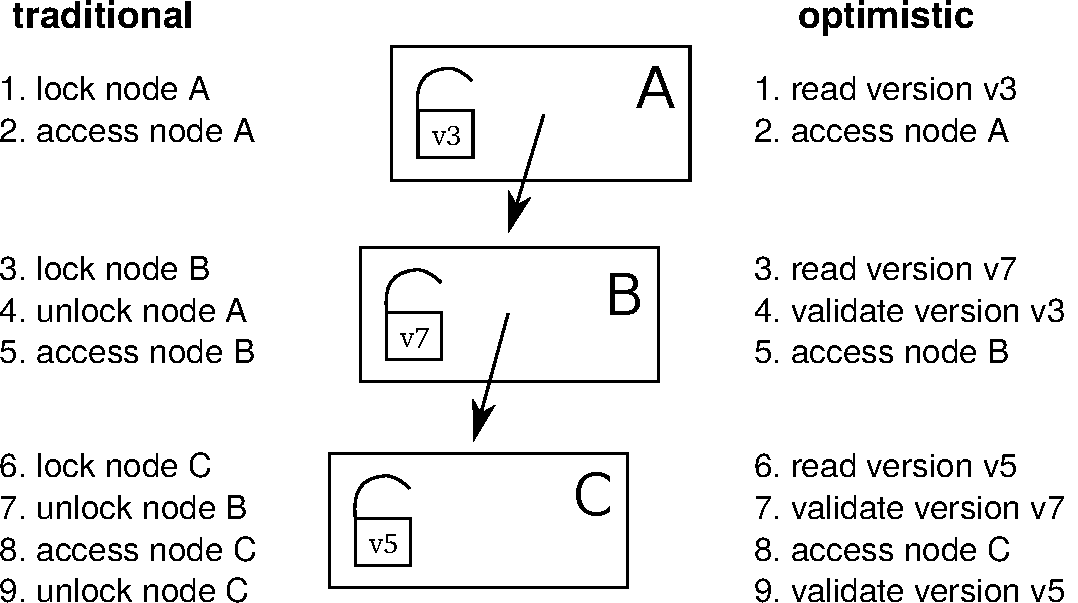
\includegraphics[width=0.65\linewidth]{olcall.pdf}
  \vspace{0.2cm}
  \caption{Comparison of a lookup operation in a 3-level tree using traditional lock coupling (left-hand side) vs.~optimistic lock coupling (right-hand side).}
  \label{fig:olc}
\end{figure}

The traditional and most common lock-based synchronization protocol for B-trees is lock coupling, which interleaves lock acquisitions while holding at most two locks at a time.
If, as we observed earlier, optimistic locks have similar semantics as traditional locks, it is natural to ask whether lock coupling can be combined with optimistic locks.
And indeed the answer is yes: One can almost mechanically translate traditional lock coupling code to optimistic lock coupling code.
This is illustrated in Figure~\ref{fig:olc}, which compares the traversal in a tree of height 3 using traditional and optimistic locks.
As the figure shows, the main difference is that locking is translated to reading the version and that unlocking becomes validation of the previously read version.
This simple change provides efficient lock-free tree traversal without the need to design a complex synchronization protocol.

It is important to emphasize the conceptual simplicity of OLC in comparison to data structures that use custom protocols like the Bw-tree~\cite{DBLP:conf/icde/LevandoskiLS13a}.
To implement lock-free access, the Bw-tree requires an indirection table, delta nodes, complex splitting and merging logic, retry logic, etc.
OLC, on the other hand, can directly be applied to B-trees mostly by adding the appropriate optimistic locking code and without modifying the node layout itself.
Therefore, OpenBw-Tree, an open source implementation of the Bw-tree, requires an order of magnitude more code than a B-tree based on OLC\footnote{Both implementations are available on GitHub: \url{https://github.com/wangziqi2016/index-microbench}}.
Given how difficult it is to develop, validate, and debug lock-free code, simplicity is obviously a major advantage.

\subsection{Correctness Aspects}

\begin{figure}
  % \centering
  %[basicstyle=\normalsize\ttfamily,showstringspaces=false,columns=fullflexible,breaklines=false,breakatwhitespace=true,numbers=none,numberstyle=\small,style=C,keepspaces=true]
\begin{lstlisting}[basicstyle=\ttfamily,language=C++,numbers=left,numberstyle=\small]
std::atomic<BTreeNode*> root;

// search for key in B+tree, returns payload in resultOut
bool lookup(Key key, Value& resultOut) {
   BTreeNode* node = root.load();
   uint64_t nodeVersion = node->readLockOrRestart();
   if (node != root.load()) // make sure the root is still the root
      restart();

   BTreeInner<Key>* parent = nullptr;
   uint64_t parentVersion = 0;

   while (node->isInner()) {
      auto inner = (BTreeInner*)node;

      // unlock parent and make current node the parent
      if (parent)
         parent->readUnlockOrRestart(parentVersion);
      parent = inner;
      parentVersion = nodeVersion;

      // search for next node
      node = inner->findChild(key);
      // validate 'inner' to ensure that 'node' pointer is valid
      inner->checkOrRestart(nodeVersion);
      // now it safe to dereference 'node' pointer (read its version)
      nodeVersion = node->readLockOrRestart();
   }

   // search in leaf and retrieve payload
   auto leaf = (BTreeLeaf*)node;
   bool success = leaf->findValue(key, resultOut);

   // unlock everything
   if (parent)
      parent->readUnlockOrRestart(parentVersion);
   node->readUnlockOrRestart(nodeVersion);

   return success;
}
\end{lstlisting}
  \vspace{0.2cm}
  \caption{B-tree lookup code using OLC. For simplicity, the restart logic is not shown.}
  \label{fig:lookup}
\end{figure}

So far, we have introduced the high-level ideas behind OLC and have stressed its similarity to traditional lock coupling.
Let us now discuss some cases where the close similarity between lock coupling and OLC breaks down.
To make this more concrete, we show the B-tree lookup code in Figure~\ref{fig:lookup}.
In the code, \texttt{readLockOrRestart} reads the lock version and \texttt{readUnlockOrRestart} validates that the read was correct.

One issue with OLC is that any pointer speculatively read from a node may point to invalid memory (if that node is modified concurrently).
Dereferencing such a pointer (e.g., to read its optimistic lock), may cause a segmentation fault or undefined behavior.
In the code shown in Figure~\ref{fig:lookup}, this problem is prevented by the extra check in line 25, which ensures that the read from the node containing the pointer was correct.
Without this additional validation, the code would in line 27 dereference the pointer speculatively read in line 23.
Note that the implementation of \texttt{checkOrRestart} is actually identical to \texttt{readUnlockOrRestart}.
We chose to give it a different name to highlight the fact that this extra check would not be necessary with read/write locks.

Another potential issue with optimistic locks is code that does not terminate.
Code that speculatively accesses a node, like an intra-node binary search, should be written in a way such that it always terminates---even in the presence of concurrent writes.
Otherwise, the validation code that detects the concurrent write will never run.
The binary search of a B-tree, for example, needs to be written in such a way that each comparison makes progress.
For some data structures that do not require loops in the traversal code (like ART) termination is trivially true.

\subsection{Implementation Details}

% implementation, efficiency
To implement an optimistic lock, one can combine the lock and the version counter into a single 64-bit\footnote{Even after subtracting one bit for the lock status, a back-of-the-envelope calculation can show that 63 bits are large enough to never overflow in practice.} word~\cite{artsync}.
A typical read operation will therefore merely consist of reading this version counter atomically.
In C++11 this can be implemented using the \texttt{std::atomic} type.

On x86, atomic reads are cheap because of x86's strong memory order guarantees.
No memory fences are required for sequentially-consistent loads, which are translated (by both GCC and clang) into standard \texttt{MOV} instructions.
Hence, the only effect of \texttt{std::atomic} for loads is preventing instruction re-ordering.
This makes version access and validation cheap.
Acquiring and releasing an optimistic lock in exclusive mode has comparable cost to a traditional lock:
A fairly expensive sequentially-consistent store is needed for acquiring a lock, while a standard \texttt{MOV} suffices for releasing it.
A simple sinlock-based implementation of optimistic locks can be found in the appendix of an earlier paper~\cite{artsync}.

OLC code must be able to handle restarts since validation or lock upgrade can fail due to concurrent writers.
Restarts can easily be implemented by wrapping the data structure operation in a loop (for simplicity not shown in Figure~\ref{fig:lookup}).
Such a loop also enables limiting the number of optimistic retry operations and falling back to pessimistic locking in cases of very heavy contention.
The ability to fall back to traditional locking is a major advantage of OLC in terms of robustness over lock-free approaches, which do not have this option.

In addition to the optimistic shared mode and the exclusive mode, optimistic locks also support a ``shared pessimistic'' mode, which physically acquires the lock in shared mode (allowing multiple concurrent readers but no writers).
This mode is useful for table (or range) scans that touch many tuples on a leaf page (which would otherwise easily abort).
Finally, let us mention that large range scans and table scans, should be broken up into several per-node traversals as is done in the LeanStore~\cite{leanstore} system.

Like all lock-free data structures, but unlike traditional locking and Hardware Transactional Memory~\cite{DBLP:conf/hpca/KarnagelDRLLSL14,DBLP:journals/pvldb/MakreshanskiLS15,htmtkde}, OLC requires care when deleting (and reusing) nodes.
The reason is that a deleting thread can never be sure that a node can be reclaimed because other threads might still be optimistically reading from that node.
Therefore, standard solutions like epoch-based reclamation~\cite{DBLP:conf/sosp/TuZKLM13}, hazard pointers~\cite{DBLP:journals/tpds/Michael04}, or optimized hazard pointers~\cite{DBLP:conf/spaa/BalmauGHZ16} need to be used.
These memory reclamation techniques are, however, largely orthogonal to the synchronization protocol itself.

%-lock-free is not a strong guarantee

\newpage
\section{Evaluation}\label{sec:evaluation}

Let us now experimentally evaluate the overhead and scalability of OLC.
For the experiments, we use an in-memory B+tree implemented in C++11 using templates, which is configured to use nodes of 4096 bytes, random 8 byte keys, and 8 byte payloads.
Based on this B-tree, we compare the following synchronization approaches:
\begin{itemize}
\item an OLC implementation\footnote{An almost identical OLC implementation is available on github: \url{https://github.com/wangziqi2016/index-microbench/tree/master/BTreeOLC}}
\item a variant based on traditional lock coupling and read/write locks
\item the unsynchronized B-tree, which obviously is only correct for read-only workloads but allows measuring the overhead of synchronization
\end{itemize}
Note that earlier work has compared the OLC implementation with a Bw-tree implementation~\cite{buzzword} and other state-of-the-art in-memory index structures.

We use a Haswell EP system with an Intel Xeon E5-2687W v3 CPU, which has 10 cores (20 ``Hyper-Threads'') and 25~MB of L3 cache.
The system is running Ubuntu 18.10 and we use GCC 8.2.0 to compile our code.
The CPU counters are obtained using the Linux perf API\footnote{We use the following convenience wrapper: \url{https://github.com/viktorleis/perfevent}}.

\begin{table}
  \caption{Performance and CPU counters for lookup and insert operations in a B-tree with 100M keys. We perform 100M operations and normalize the CPU counters by that number.}
  \label{tab:overhead}
  \centering
  \begin{tabular}{lrrrrrrr}\toprule
                    &         &        &        & instruc-  & L1     & L3     & branch \\
                    & threads & M op/s & cycles & tions & misses & misses & misses \\\midrule
lookup (no sync.)   & 1       & 1.72   & 2028   & 283     & 39.1   & 14.9   & 16.1   \\
lookup (OLC)        & 1       & 1.65   & 2107   & 370     & 43.9   & 15.1   & 16.7   \\
lookup (lock coup.) & 1       & 1.72   & 2078   & 365     & 42.3   & 16.9   & 15.7   \\\midrule
insert (no sync.)   & 1       & 1.51   & 2286   & 530     & 59.8   & 31.1   & 17.3   \\
insert (OLC)        & 1       & 1.50   & 2303   & 629     & 61.2   & 31.1   & 16.5   \\
insert (lock coup.) & 1       & 1.41   & 2473   & 644     & 61.0   & 31.0   & 17.2   \\\midrule
lookup (no sync.)   & 10      & 15.48  & 2058   & 283     & 38.6   & 15.5   & 16.0   \\
lookup (OLC)        & 10      & 14.60  & 2187   & 370     & 43.8   & 15.8   & 16.8   \\
lookup (lock coup.) & 10      & 5.71   & 5591   & 379     & 54.2   & 17.0   & 14.8   \\\midrule
insert (no sync.)   & 10      & -      & -      & -       & -      & -      & -      \\
insert (OLC)        & 10      & 10.46  & 2940   & 656     & 62.0   & 32.5   & 16.8   \\
insert (lock coup.) & 10      & 7.55   & 4161   & 667     & 75.0   & 28.6   & 16.2   \\
    \bottomrule
\end{tabular}
\end{table}

Table~\ref{tab:overhead} compares the performance and CPU counters for lookup and insert operations in a B-tree with 100M keys.
With {\em single-threaded} execution, we observe that all three approaches have very similar performance.
Adding traditional or optimistic locks to unsynchronized B-tree code results in up to 30\% of additional instructions without affecting single-threaded performance much.

\begin{figure}
  \centering
  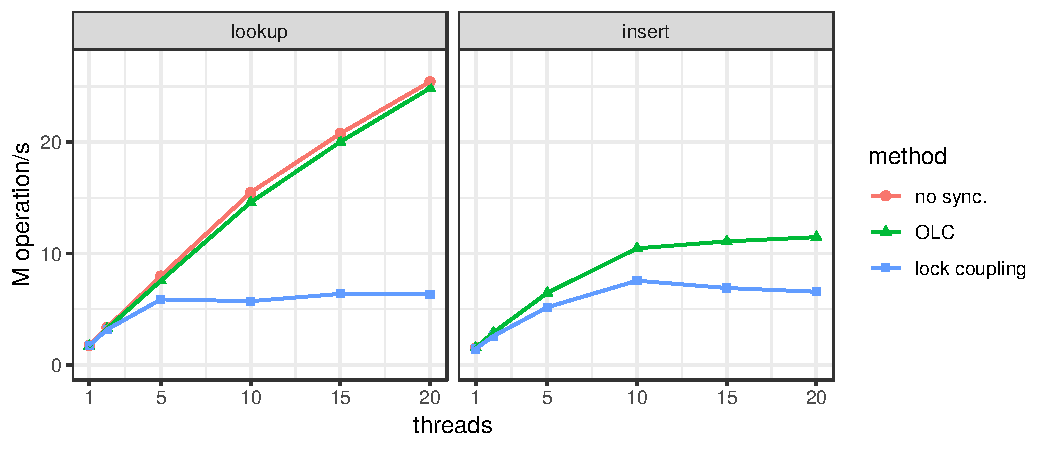
\includegraphics[width=\linewidth]{scale.pdf}
  \vspace{0.2cm}
  \caption{Scalability on 10-core system for B-tree operations (100M values).}
  \label{fig:scale}
\end{figure}

As Figure~\ref{fig:scale} shows, the results change dramatically once we use multiple threads.
For lookup, the scalability of OLC is near-linear up to 20 threads, even though the system has only 10 ``real cores''.
The OLC scalability for insert is also respectable (though not quite as linear because multi-threaded insertion approaches the memory bandwidth of our processor).
The figure also shows that the results of traditional lock coupling with read/write locks are significantly worse than OLC.
With 20 threads, lookup with OLC is 3.9$\times$ faster than traditional lock coupling.

\section{Summary}\label{sec:conc}

Optimistic Lock Coupling (OLC) is an effective synchronization method that combines the simplicity of traditional lock coupling with the superior scalability of lock-free approaches.
OLC is widely applicable and has already been successfully used to synchronize several data structures, including B-trees, binary search trees, and different trie variants.
These features make it highly attractive for modern database systems as well as performance-critical systems software in general.

\begin{thebibliography}{10}

\bibitem{DBLP:conf/spaa/BalmauGHZ16}
O.~Balmau, R.~Guerraoui, M.~Herlihy, and I.~Zablotchi.
\newblock Fast and robust memory reclamation for concurrent data structures.
\newblock In {\em SPAA}, 2016.

\bibitem{DBLP:journals/acta/BayerS77}
R.~Bayer and M.~Schkolnick.
\newblock Concurrency of operations on {B}-trees.
\newblock {\em Acta Informatica}, 9, 1977.

\bibitem{hot}
R.~Binna, E.~Zangerle, M.~Pichl, G.~Specht, and V.~Leis.
\newblock {HOT}: A height optimized trie index for main-memory database
  systems.
\newblock In {\em SIGMOD}, 2018.

\bibitem{DBLP:conf/ppopp/BronsonCCO10}
N.~G. Bronson, J.~Casper, H.~Chafi, and K.~Olukotun.
\newblock A practical concurrent binary search tree.
\newblock In {\em PPOPP}, 2010.

\bibitem{DBLP:conf/vldb/ChaHKK01}
S.~K. Cha, S.~Hwang, K.~Kim, and K.~Kwon.
\newblock Cache-conscious concurrency control of main-memory indexes on
  shared-memory multiprocessor systems.
\newblock In {\em VLDB}, 2001.

\bibitem{intel}
I.~Cutress.
\newblock {Intel} goes for 48-cores: {Cascade-AP} with multi-chip package
  coming soon.
\newblock
  \url{https://www.anandtech.com/show/13535/intel-goes-for-48cores-cascade-ap},
  2018 (accessed January, 2019).

\bibitem{DBLP:conf/cidr/FaleiroA17}
J.~M. Faleiro and D.~J. Abadi.
\newblock Latch-free synchronization in database systems: Silver bullet or
  fool's gold?
\newblock In {\em CIDR}, 2017.

\bibitem{DBLP:journals/ftdb/Graefe11}
G.~Graefe.
\newblock Modern {B}-tree techniques.
\newblock {\em Foundations and Trends in Databases}, 3(4), 2011.

\bibitem{DBLP:conf/hpca/KarnagelDRLLSL14}
T.~Karnagel, R.~Dementiev, R.~Rajwar, K.~Lai, T.~Legler, B.~Schlegel, and
  W.~Lehner.
\newblock Improving in-memory database index performance with
  {Intel}\({}^{\mbox{{\textregistered}}}\) transactional synchronization
  extensions.
\newblock In {\em HPCA}, 2014.

\bibitem{DBLP:journals/tods/LehmanY81}
P.~L. Lehman and S.~B. Yao.
\newblock Efficient locking for concurrent operations on {B}-trees.
\newblock {\em {ACM} Trans. Database Syst.}, 6(4), 1981.

\bibitem{leanstore}
V.~Leis, M.~Haubenschild, A.~Kemper, and T.~Neumann.
\newblock Leanstore: In-memory data management beyond main memory.
\newblock In {\em ICDE}, 2018.

\bibitem{art}
V.~Leis, A.~Kemper, and T.~Neumann.
\newblock The adaptive radix tree: {ARTful} indexing for main-memory databases.
\newblock In {\em ICDE}, 2013.

\bibitem{htmtkde}
V.~Leis, A.~Kemper, and T.~Neumann.
\newblock Scaling {HTM}-supported database transactions to many cores.
\newblock {\em {IEEE} Trans. Knowl. Data Eng.}, 28(2), 2016.

\bibitem{artsync}
V.~Leis, F.~Scheibner, A.~Kemper, and T.~Neumann.
\newblock The {ART} of practical synchronization.
\newblock In {\em DaMoN}, 2016.

\bibitem{DBLP:conf/icde/LevandoskiLS13a}
J.~J. Levandoski, D.~B. Lomet, and S.~Sengupta.
\newblock The {Bw}-tree: A {B}-tree for new hardware platforms.
\newblock In {\em ICDE}, 2013.

\bibitem{DBLP:journals/pvldb/MakreshanskiLS15}
D.~Makreshanski, J.~J. Levandoski, and R.~Stutsman.
\newblock To lock, swap, or elide: On the interplay of hardware transactional
  memory and lock-free indexing.
\newblock {\em {PVLDB}}, 8(11), 2015.

\bibitem{DBLP:dblp_conf/eurosys/MaoKM12}
Y.~Mao, E.~Kohler, and R.~T. Morris.
\newblock Cache craftiness for fast multicore key-value storage.
\newblock In {\em EuroSys}, 2012.

\bibitem{DBLP:journals/tpds/Michael04}
M.~M. Michael.
\newblock Hazard pointers: Safe memory reclamation for lock-free objects.
\newblock {\em {IEEE} Trans. Parallel Distrib. Syst.}, 15(6), 2004.

\bibitem{DBLP:journals/jacm/ShalevS06}
O.~Shalev and N.~Shavit.
\newblock Split-ordered lists: Lock-free extensible hash tables.
\newblock {\em J. {ACM}}, 53(3), 2006.

\bibitem{amd}
A.~Shilov.
\newblock {AMD} previews {EPYC} ‘{Rome}’ processor: Up to 64 {Zen} 2 cores.
\newblock
  \url{https://www.anandtech.com/show/13561/amd-previews-epyc-rome-processor-up-to-64-zen-2-cores},
  2018 (accessed January, 2019).

\bibitem{DBLP:conf/sosp/TuZKLM13}
S.~Tu, W.~Zheng, E.~Kohler, B.~Liskov, and S.~Madden.
\newblock Speedy transactions in multicore in-memory databases.
\newblock In {\em SOSP}, 2013.

\bibitem{buzzword}
Z.~Wang, A.~Pavlo, H.~Lim, V.~Leis, H.~Zhang, M.~Kaminsky, and D.~Andersen.
\newblock Building a {Bw}-tree takes more than just buzz words.
\newblock In {\em SIGMOD}, 2018.

\end{thebibliography}


%\bibliographystyle{abbrv}
%\bibliography{main}

\end{document}

\end{article}

\begin{article}
{College-Related Question Answering based on Knowledge Graph}
{Cheng Peng,  Hao Jiang, Junnan Dong, and Xiao Huang}
%\graphicspath{{submissions/NobleRoberts_final/}}
\pdfminorversion=5
\documentclass[11pt]{article}
\usepackage{deauthor,times,graphicx,caption,microtype}
\usepackage{hyperref}
\usepackage{listings}
\usepackage{booktabs}

\begin{document}

\title{Optimistic Lock Coupling: A Scalable and Efficient General-Purpose Synchronization Method}

\author{Viktor Leis, Michael Haubenschild\raisebox{0.9ex}{$\ast$}, Thomas Neumann\\ Technische Universit{\"a}t M{\"u}nchen \hspace{0.7cm} Tableau Software\raisebox{0.9ex}{$\ast$} \\ {\{leis,neumann\}{@}in.tum.de} \hspace{0.7cm} {mhaubenschild{@}tableau.com\raisebox{0.9ex}{$\ast$}}}

\maketitle

\begin{abstract}
As the number of cores on commodity processors continues to increase, scalability becomes more and more crucial for overall performance.
Scalable and efficient concurrent data structures are particularly important, as these are often the building blocks of parallel algorithms.
Unfortunately, traditional synchronization techniques based on fine-grained locking have been shown to be unscalable on modern multi-core CPUs.
Lock-free data structures, on the other hand, are extremely difficult to design and often incur significant overhead.

In this work, we make the case for Optimistic Lock Coupling as a practical alternative to both traditional locking and the lock-free approach.
We show that Optimistic Lock Coupling is highly scalable and almost as simple to implement as traditional lock coupling.
Another important advantage is that it is easily applicable to most tree-like data structures.
We therefore argue that Optimistic Lock Coupling, rather than a complex and error-prone custom synchronization protocol, should be the default choice for performance-critical data structures.
\end{abstract}

\section{Introduction}

% more and more cores
Today, Intel's commodity server processors have up to 28 cores and its upcoming microarchitecture will have up to 48 cores per socket~\cite{intel}.
Similarly, AMD currently stands at 32 cores and this number is expected to double in the next generation~\cite{amd}.
Since both platforms support simultaneous multithreading (also known as hyperthreading), affordable commodity servers (with up to two sockets) will soon routinely have between 100 and 200 hardware threads.

% data structure scalability is important
With such a high degree of hardware parallelism, efficient data processing crucially depends on how well concurrent data structures scale.
Internally, database systems use a plethora of data structures like table heaps, internal work queues, and, most importantly, index structures.
Any of these can easily become a scalability (and therefore overall performance) bottleneck on many-core CPUs.

% traditional synchronization: fine-grained locks, slow, cache invalidation
Traditionally, database systems synchronize internal data structures using fine-grained reader/writer locks\footnote{In this work, we focus on data structure synchronization rather than high-level transaction semantics and therefore use the term {\em lock} for what would typically be called {\em latch} in the database literature. We thus follow common computer science (rather than database) terminology.}.
Unfortunately, while fine-grained locking makes lock contention unlikely, it still results in bad scalability because lock acquisition and release require writing to shared memory.
Due to the way cache coherency is implemented on modern multi-core CPUs, these writes cause additional cache misses\footnote{The cache coherency protocol ensures that all copies of a cache line on other cores are invalidated before the write can proceed.} and the cache line containing the lock's internal data becomes a point of physical contention.
As a result, any frequently-accessed lock (e.g., the lock of the root node of a B-tree) severely limits scalability.

% lock-free bw-tree: no more latches, but indirections, extremely complex
Lock-free data structures like the Bw-tree~\cite{DBLP:conf/icde/LevandoskiLS13a} (a lock-free B-tree variant) or the Split-Ordered List~\cite{DBLP:journals/jacm/ShalevS06} (a lock-free hash table) do not acquire any locks and therefore generally scale much better than locking-based approaches (in particular for read-mostly workloads).
However, lock-free synchronization has other downsides:
First, it is very difficult and results in extremely complex and error-prone code (when compared to locking).
Second, because the functionality of atomic primitives provided by the hardware (e.g., atomically compare-and-swap 8 bytes) is limited, complex operations require additional indirections within the data structure.
For example, the Bw-tree requires an indirection table and the Split-Ordered List requires ``dummy nodes'', resulting in overhead due to additional cache misses.

% OLC for the win
In this paper we make the case for {\em Optimistic Lock Coupling (OLC)}, a synchronization method that combines some of the best properties of lock-based and lock-free synchronization.
OLC utilizes a special lock type that can be used in two modes:
The first mode is similar to a traditional mutex and excludes other threads by physically acquiring the underlying lock.
In the second mode, reads can proceed optimistically by validating a version counter that is embedded in the lock (similar to optimistic concurrency control).
The first mode is typically used by writers and the second mode by readers.
Besides this special lock type, OLC is based on the observation that optimistic lock validations can be interleaved/coupled---similar to the pair-wise interleaved lock acquisition of traditional lock coupling.
Hence, the name Optimistic Lock Coupling.

OLC has a number of desirable features:
\begin{itemize}
\item By reducing the number of writes to shared memory locations and thereby avoiding cache invalidations, it {\bf scales well} for most workloads.
\item In comparison to unsynchronized code, it requires few additional CPU instructions making it {\bf efficient}.
\item OLC is {\bf widely applicable} to different data structures. It has already been successfully used for synchronizing binary search trees~\cite{DBLP:conf/ppopp/BronsonCCO10}, tries~\cite{artsync}, trie/B-tree hybrids~\cite{DBLP:dblp_conf/eurosys/MaoKM12}, and B-trees~\cite{buzzword}.
\item In comparison to the lock-free paradigm, it is also {\bf easy to use} and requires few modifications to existing, single-threaded data structures.
\end{itemize}
Despite these positive features and its simplicity, OLC is not yet widely known.
The goal of this paper is therefore to popularize this simple idea and to make a case for it.
We argue that OLC deserves to be widely known.
It is a good default synchronization paradigm---more complex, data structure-specific protocols are seldom beneficial.

The rest of the paper is organized as follows.
Section~\ref{sec:related} discusses related work, tracing the history of OLC and its underlying ideas in the literature.
The core of the paper is Section~\ref{sec:olc}, which describes the ideas behind OLC and how it can be used to synchronize complex data structures.
In Section~\ref{sec:evaluation} we experimentally show that OLC has low overhead and scales well when used to synchronize an in-memory B-tree.
We summarize the paper in Section~\ref{sec:conc}.

\newpage
\section{Related Work}\label{sec:related}

Lock coupling has been proposed as a method for allowing concurrent operations on B-trees in 1977~\cite{DBLP:journals/acta/BayerS77}.
This traditional and still widely-used method, described in detail in Graefe's B-tree survey~\cite{DBLP:journals/ftdb/Graefe11}, is also called ``latch coupling'', ``hand-over-hand locking'', and ``crabbing''.
Because at most two locks are held at-a-time during tree traversal, this technique seemingly allows for a high degree of parallelism---in particular if read/write locks are used to enable inner nodes to be locked in shared mode.
However, as we show in Section~\ref{sec:evaluation}, on modern hardware lock acquisition (even in shared mode) results in suboptimal scalability.

An early alternative from 1981 is a B-tree variant called B-link tree~\cite{DBLP:journals/tods/LehmanY81}, which only holds a single lock at a time.
It is based on the observation that between the release of the parent lock and the acquisition of the child lock, the only ``dangerous'' thing that could have happened is the split of a child node (assuming one does not implement merge operations).
Thus, when a split happens, the key being searched might end up on a neighboring node to the right of the current child node.
A B-link tree traversal therefore detects this condition and, if needed, transparently proceeds to the neighboring node.
Releasing the parent lock early is highly beneficial when the child node needs to be fetched from disk.
For in-memory workloads, however, the B-link tree has the same scalability issues as lock coupling (it acquires just as many locks).

The next major advance, Optimistic Latch-Free Index Traversal (OLFIT)~\cite{DBLP:conf/vldb/ChaHKK01}, was proposed in 2001.
OLFIT introduced the idea of a combined lock/update counter, which we call {\em optimistic lock}. % , for lack of a better name,
Based on these per-node optimistic locks and the synchronization protocol of the B-link tree, OLFIT finally achieves good scalability on parallel processors.
The OLFIT protocol is fairly complex, as it requires both the non-trivial B-link protocol and optimistic locks.
Furthermore, like the B-link tree protocol, it does not support merging nodes, and is specific to B-trees (cannot easily be applied to other data structures).

In the following two decades, the growth of main-memory capacity led to much research into other data structures besides the venerable B-tree.
Particularly relevant for our discussion is Bronson et al.'s~\cite{DBLP:conf/ppopp/BronsonCCO10} concurrent binary search tree, which is based on optimistic version validation and has a sophisticated, data structure-specific synchronization protocol.
To the best of our knowledge, this 2010 paper is the first that, as part of its protocol, interleaves version validation across nodes---rather than validating each node separately like OLFIT.
In that paper, this idea is called ``hand-over-hand, optimistic validation'', while we prefer the term Optimistic Lock Coupling to highlight the close resemblance to traditional lock coupling.
Similarly, Mao et al.'s~\cite{DBLP:dblp_conf/eurosys/MaoKM12} Masstree (a concurrent hybrid trie/B-tree) is also based on the same ideas, but again uses them as part of a more complex protocol.

The Adaptive Radix Tree (ART)~\cite{art} is another recent in-memory data structure, which we proposed in 2013.
In contrast to the two data structures just mentioned, it was originally designed with single-threaded performance in mind without supporting concurrency.
To add support for concurrency, we initially started designing a custom protocol called Read-Optimized Write Exclusion (ROWEX)~\cite{artsync}, which turned out to be non-trivial and requires modifications of the underlying data structure\footnote{Note that ROWEX is already easier to apply to existing data structures than the lock-free approach. The difficulty depends on the data structure. Applying ROWEX is hard for B-trees with sorted keys and fairly easy for copy-on-write data structures like the Height Optimized Trie~\cite{hot}---with ART being somewhere in the middle.}.
However, fairly late in the project, we also realized, that OLC {\em alone} (rather than as part of a more complex protocol) is sufficient to synchronize ART.
No other changes to the data structure were necessary.
Both approaches were published and experimentally evaluated in a followup paper~\cite{artsync}, which shows that, despite its simplicity, OLC is efficient, scalable, and generally outperforms ROWEX.

Similar results were recently published regarding B-trees~\cite{buzzword}.
In this experimental study a simple OLC-based synchronization outperformed the Bw-tree~\cite{DBLP:conf/icde/LevandoskiLS13a}, a complex lock-free synchronization approach.
Another recent paper shows that for write-intensive workloads, locking often performs better than lock-free synchronization~\cite{DBLP:conf/cidr/FaleiroA17}.
These experiences indicate that OLC is a general-purpose synchronization paradigm and motivate the current paper.

%foster b-tree\cite{DBLP:journals/tods/GraefeKK12}
%Shasha theory~\cite{DBLP:journals/tods/ShashaG88}

\section{Optimistic Lock Coupling}\label{sec:olc}

% locks suck
The standard technique for inter-thread synchronization is mutual exclusion using fine-grained locks.
In a B-tree, for example, every node usually has its own associated lock, which is acquired before accessing that node.
The problem of locking on modern multi- and many-core processors is that lock acquisition and release require writing to the shared memory location that implements the lock.
This write causes exclusive ownership of the underlying cache line and invalidates copies of it on all other processor cores.
For hierarchical, tree-like data structures, the lock of the root node becomes a point of physical contention---even in read-only workloads and even when read/write locks are used.
Depending on the specific data structure, number of cores, cache coherency protocol implementation, cache topology, whether Non-Uniform Memory Access (NUMA) is used, locking can even result in multi-threaded performance that is worse than single-threaded execution.

% in b-trees this happens very much
The inherent pessimism of locking is particularly unfortunate for B-trees:
Despite the fact that logical modifications of the root node are very infrequent, every B-tree operation must lock the root node during tree traversal\footnote{To a lesser extent this obviously applies to all inner nodes, not just the root.}.
Even the vast majority of update operations (with the exception of splits and merges), only modify a single leaf node.
These observations indicate that a more optimistic approach, which does not require locking inner nodes, would be very beneficial for B-trees.

\subsection{Optimistic Locks}

% optimism to the rescue
As the name indicates, optimistic locks try to solve the scalability issues of traditional locks using an optimistic approach.
Instead of always physically acquiring locks, even for nodes that are unlikely to be modified simultaneously, after-the-fact validation is used to detect conflicts.
This is done by augmenting each lock with a version/update counter that is incremented on every modification.
Using this version counter, readers can optimistically proceed before validating that the version did not change to ensure that the read was safe.
If validation fails, the operation is restarted.

% details on opt locks
Using optimistic locks, a read-only node access (i.e., the majority of all operations in a B-tree) does not acquire the lock and does not increment the version counter.
Instead, it performs the following steps:
\begin{enumerate}
\item read lock version (restart if lock is not free)
\item access node
\item read the version again and validate that it has not changed in the meantime
\end{enumerate}
If the last step (the validation) fails, the operation has to be restarted.
Write operations, on the other hand, are more similar to traditional locking:
\begin{enumerate}
\item acquire lock (wait if necessary)
\item access/write to node
\item increment version and unlock node
\end{enumerate}
Writes can therefore protect a node from other writes.

% similar to locks
As we observed in an earlier paper~\cite{artsync}, because of similar semantics, optimistic locks can be hidden behind an API very similar to traditional read/write locks.
Both approaches have an exclusive lock mode, and acquiring a traditional lock in shared mode is analogous to optimistic version validation.
Furthermore, like with some implementations of traditional read/write locks, optimistic locks allow upgrading a shared lock to an exclusive lock.
Lock upgrades are, for example, used to avoid most B-tree update operations from having to lock inner nodes.
In our experience, the close resemblance of optimistic and traditional locks simplifies the reasoning about optimistic locks;
one can apply similar thinking as in traditional lock-based protocols.

\subsection{Lock Coupling with Optimistic Locks}

\begin{figure}
  \centering
  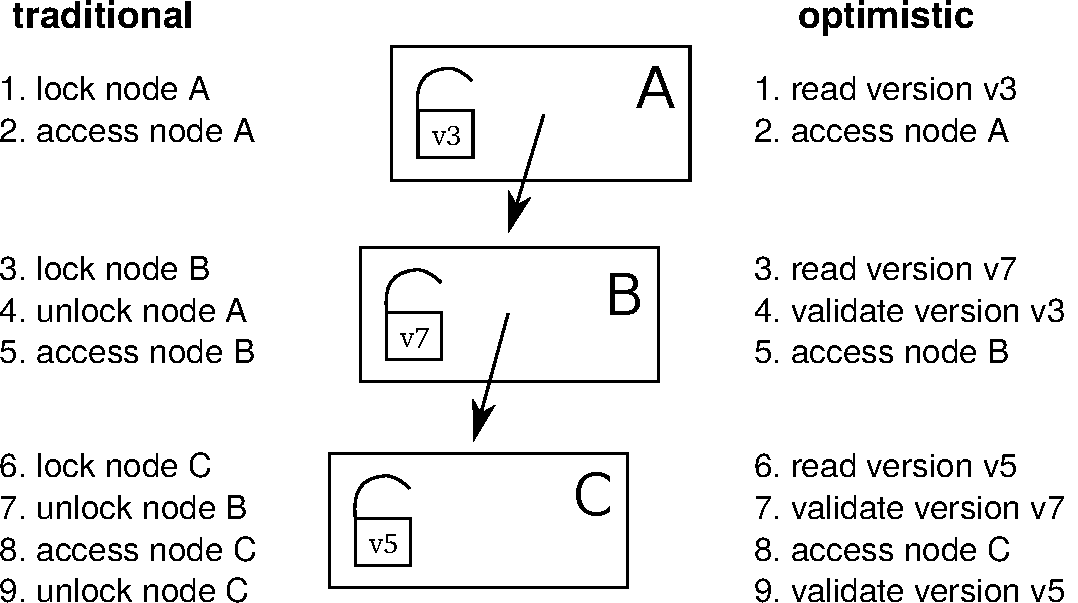
\includegraphics[width=0.65\linewidth]{olcall.pdf}
  \vspace{0.2cm}
  \caption{Comparison of a lookup operation in a 3-level tree using traditional lock coupling (left-hand side) vs.~optimistic lock coupling (right-hand side).}
  \label{fig:olc}
\end{figure}

The traditional and most common lock-based synchronization protocol for B-trees is lock coupling, which interleaves lock acquisitions while holding at most two locks at a time.
If, as we observed earlier, optimistic locks have similar semantics as traditional locks, it is natural to ask whether lock coupling can be combined with optimistic locks.
And indeed the answer is yes: One can almost mechanically translate traditional lock coupling code to optimistic lock coupling code.
This is illustrated in Figure~\ref{fig:olc}, which compares the traversal in a tree of height 3 using traditional and optimistic locks.
As the figure shows, the main difference is that locking is translated to reading the version and that unlocking becomes validation of the previously read version.
This simple change provides efficient lock-free tree traversal without the need to design a complex synchronization protocol.

It is important to emphasize the conceptual simplicity of OLC in comparison to data structures that use custom protocols like the Bw-tree~\cite{DBLP:conf/icde/LevandoskiLS13a}.
To implement lock-free access, the Bw-tree requires an indirection table, delta nodes, complex splitting and merging logic, retry logic, etc.
OLC, on the other hand, can directly be applied to B-trees mostly by adding the appropriate optimistic locking code and without modifying the node layout itself.
Therefore, OpenBw-Tree, an open source implementation of the Bw-tree, requires an order of magnitude more code than a B-tree based on OLC\footnote{Both implementations are available on GitHub: \url{https://github.com/wangziqi2016/index-microbench}}.
Given how difficult it is to develop, validate, and debug lock-free code, simplicity is obviously a major advantage.

\subsection{Correctness Aspects}

\begin{figure}
  % \centering
  %[basicstyle=\normalsize\ttfamily,showstringspaces=false,columns=fullflexible,breaklines=false,breakatwhitespace=true,numbers=none,numberstyle=\small,style=C,keepspaces=true]
\begin{lstlisting}[basicstyle=\ttfamily,language=C++,numbers=left,numberstyle=\small]
std::atomic<BTreeNode*> root;

// search for key in B+tree, returns payload in resultOut
bool lookup(Key key, Value& resultOut) {
   BTreeNode* node = root.load();
   uint64_t nodeVersion = node->readLockOrRestart();
   if (node != root.load()) // make sure the root is still the root
      restart();

   BTreeInner<Key>* parent = nullptr;
   uint64_t parentVersion = 0;

   while (node->isInner()) {
      auto inner = (BTreeInner*)node;

      // unlock parent and make current node the parent
      if (parent)
         parent->readUnlockOrRestart(parentVersion);
      parent = inner;
      parentVersion = nodeVersion;

      // search for next node
      node = inner->findChild(key);
      // validate 'inner' to ensure that 'node' pointer is valid
      inner->checkOrRestart(nodeVersion);
      // now it safe to dereference 'node' pointer (read its version)
      nodeVersion = node->readLockOrRestart();
   }

   // search in leaf and retrieve payload
   auto leaf = (BTreeLeaf*)node;
   bool success = leaf->findValue(key, resultOut);

   // unlock everything
   if (parent)
      parent->readUnlockOrRestart(parentVersion);
   node->readUnlockOrRestart(nodeVersion);

   return success;
}
\end{lstlisting}
  \vspace{0.2cm}
  \caption{B-tree lookup code using OLC. For simplicity, the restart logic is not shown.}
  \label{fig:lookup}
\end{figure}

So far, we have introduced the high-level ideas behind OLC and have stressed its similarity to traditional lock coupling.
Let us now discuss some cases where the close similarity between lock coupling and OLC breaks down.
To make this more concrete, we show the B-tree lookup code in Figure~\ref{fig:lookup}.
In the code, \texttt{readLockOrRestart} reads the lock version and \texttt{readUnlockOrRestart} validates that the read was correct.

One issue with OLC is that any pointer speculatively read from a node may point to invalid memory (if that node is modified concurrently).
Dereferencing such a pointer (e.g., to read its optimistic lock), may cause a segmentation fault or undefined behavior.
In the code shown in Figure~\ref{fig:lookup}, this problem is prevented by the extra check in line 25, which ensures that the read from the node containing the pointer was correct.
Without this additional validation, the code would in line 27 dereference the pointer speculatively read in line 23.
Note that the implementation of \texttt{checkOrRestart} is actually identical to \texttt{readUnlockOrRestart}.
We chose to give it a different name to highlight the fact that this extra check would not be necessary with read/write locks.

Another potential issue with optimistic locks is code that does not terminate.
Code that speculatively accesses a node, like an intra-node binary search, should be written in a way such that it always terminates---even in the presence of concurrent writes.
Otherwise, the validation code that detects the concurrent write will never run.
The binary search of a B-tree, for example, needs to be written in such a way that each comparison makes progress.
For some data structures that do not require loops in the traversal code (like ART) termination is trivially true.

\subsection{Implementation Details}

% implementation, efficiency
To implement an optimistic lock, one can combine the lock and the version counter into a single 64-bit\footnote{Even after subtracting one bit for the lock status, a back-of-the-envelope calculation can show that 63 bits are large enough to never overflow in practice.} word~\cite{artsync}.
A typical read operation will therefore merely consist of reading this version counter atomically.
In C++11 this can be implemented using the \texttt{std::atomic} type.

On x86, atomic reads are cheap because of x86's strong memory order guarantees.
No memory fences are required for sequentially-consistent loads, which are translated (by both GCC and clang) into standard \texttt{MOV} instructions.
Hence, the only effect of \texttt{std::atomic} for loads is preventing instruction re-ordering.
This makes version access and validation cheap.
Acquiring and releasing an optimistic lock in exclusive mode has comparable cost to a traditional lock:
A fairly expensive sequentially-consistent store is needed for acquiring a lock, while a standard \texttt{MOV} suffices for releasing it.
A simple sinlock-based implementation of optimistic locks can be found in the appendix of an earlier paper~\cite{artsync}.

OLC code must be able to handle restarts since validation or lock upgrade can fail due to concurrent writers.
Restarts can easily be implemented by wrapping the data structure operation in a loop (for simplicity not shown in Figure~\ref{fig:lookup}).
Such a loop also enables limiting the number of optimistic retry operations and falling back to pessimistic locking in cases of very heavy contention.
The ability to fall back to traditional locking is a major advantage of OLC in terms of robustness over lock-free approaches, which do not have this option.

In addition to the optimistic shared mode and the exclusive mode, optimistic locks also support a ``shared pessimistic'' mode, which physically acquires the lock in shared mode (allowing multiple concurrent readers but no writers).
This mode is useful for table (or range) scans that touch many tuples on a leaf page (which would otherwise easily abort).
Finally, let us mention that large range scans and table scans, should be broken up into several per-node traversals as is done in the LeanStore~\cite{leanstore} system.

Like all lock-free data structures, but unlike traditional locking and Hardware Transactional Memory~\cite{DBLP:conf/hpca/KarnagelDRLLSL14,DBLP:journals/pvldb/MakreshanskiLS15,htmtkde}, OLC requires care when deleting (and reusing) nodes.
The reason is that a deleting thread can never be sure that a node can be reclaimed because other threads might still be optimistically reading from that node.
Therefore, standard solutions like epoch-based reclamation~\cite{DBLP:conf/sosp/TuZKLM13}, hazard pointers~\cite{DBLP:journals/tpds/Michael04}, or optimized hazard pointers~\cite{DBLP:conf/spaa/BalmauGHZ16} need to be used.
These memory reclamation techniques are, however, largely orthogonal to the synchronization protocol itself.

%-lock-free is not a strong guarantee

\newpage
\section{Evaluation}\label{sec:evaluation}

Let us now experimentally evaluate the overhead and scalability of OLC.
For the experiments, we use an in-memory B+tree implemented in C++11 using templates, which is configured to use nodes of 4096 bytes, random 8 byte keys, and 8 byte payloads.
Based on this B-tree, we compare the following synchronization approaches:
\begin{itemize}
\item an OLC implementation\footnote{An almost identical OLC implementation is available on github: \url{https://github.com/wangziqi2016/index-microbench/tree/master/BTreeOLC}}
\item a variant based on traditional lock coupling and read/write locks
\item the unsynchronized B-tree, which obviously is only correct for read-only workloads but allows measuring the overhead of synchronization
\end{itemize}
Note that earlier work has compared the OLC implementation with a Bw-tree implementation~\cite{buzzword} and other state-of-the-art in-memory index structures.

We use a Haswell EP system with an Intel Xeon E5-2687W v3 CPU, which has 10 cores (20 ``Hyper-Threads'') and 25~MB of L3 cache.
The system is running Ubuntu 18.10 and we use GCC 8.2.0 to compile our code.
The CPU counters are obtained using the Linux perf API\footnote{We use the following convenience wrapper: \url{https://github.com/viktorleis/perfevent}}.

\begin{table}
  \caption{Performance and CPU counters for lookup and insert operations in a B-tree with 100M keys. We perform 100M operations and normalize the CPU counters by that number.}
  \label{tab:overhead}
  \centering
  \begin{tabular}{lrrrrrrr}\toprule
                    &         &        &        & instruc-  & L1     & L3     & branch \\
                    & threads & M op/s & cycles & tions & misses & misses & misses \\\midrule
lookup (no sync.)   & 1       & 1.72   & 2028   & 283     & 39.1   & 14.9   & 16.1   \\
lookup (OLC)        & 1       & 1.65   & 2107   & 370     & 43.9   & 15.1   & 16.7   \\
lookup (lock coup.) & 1       & 1.72   & 2078   & 365     & 42.3   & 16.9   & 15.7   \\\midrule
insert (no sync.)   & 1       & 1.51   & 2286   & 530     & 59.8   & 31.1   & 17.3   \\
insert (OLC)        & 1       & 1.50   & 2303   & 629     & 61.2   & 31.1   & 16.5   \\
insert (lock coup.) & 1       & 1.41   & 2473   & 644     & 61.0   & 31.0   & 17.2   \\\midrule
lookup (no sync.)   & 10      & 15.48  & 2058   & 283     & 38.6   & 15.5   & 16.0   \\
lookup (OLC)        & 10      & 14.60  & 2187   & 370     & 43.8   & 15.8   & 16.8   \\
lookup (lock coup.) & 10      & 5.71   & 5591   & 379     & 54.2   & 17.0   & 14.8   \\\midrule
insert (no sync.)   & 10      & -      & -      & -       & -      & -      & -      \\
insert (OLC)        & 10      & 10.46  & 2940   & 656     & 62.0   & 32.5   & 16.8   \\
insert (lock coup.) & 10      & 7.55   & 4161   & 667     & 75.0   & 28.6   & 16.2   \\
    \bottomrule
\end{tabular}
\end{table}

Table~\ref{tab:overhead} compares the performance and CPU counters for lookup and insert operations in a B-tree with 100M keys.
With {\em single-threaded} execution, we observe that all three approaches have very similar performance.
Adding traditional or optimistic locks to unsynchronized B-tree code results in up to 30\% of additional instructions without affecting single-threaded performance much.

\begin{figure}
  \centering
  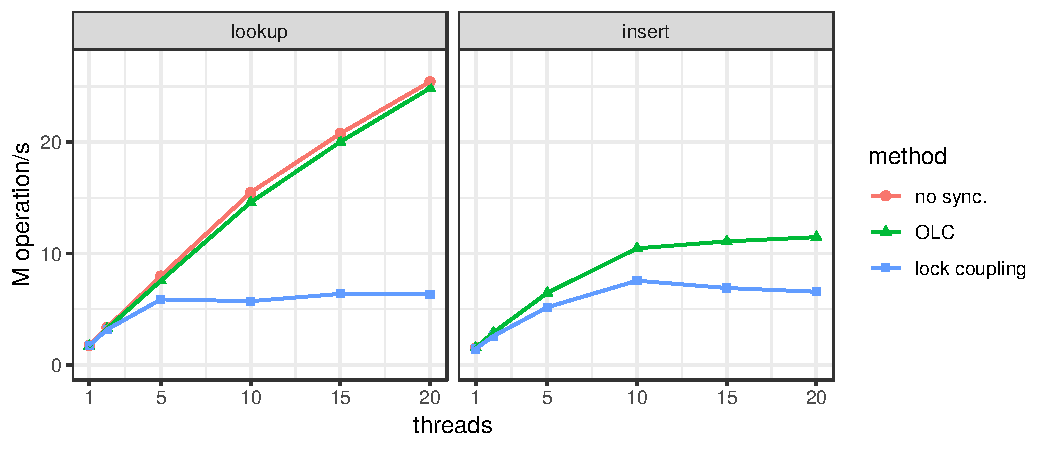
\includegraphics[width=\linewidth]{scale.pdf}
  \vspace{0.2cm}
  \caption{Scalability on 10-core system for B-tree operations (100M values).}
  \label{fig:scale}
\end{figure}

As Figure~\ref{fig:scale} shows, the results change dramatically once we use multiple threads.
For lookup, the scalability of OLC is near-linear up to 20 threads, even though the system has only 10 ``real cores''.
The OLC scalability for insert is also respectable (though not quite as linear because multi-threaded insertion approaches the memory bandwidth of our processor).
The figure also shows that the results of traditional lock coupling with read/write locks are significantly worse than OLC.
With 20 threads, lookup with OLC is 3.9$\times$ faster than traditional lock coupling.

\section{Summary}\label{sec:conc}

Optimistic Lock Coupling (OLC) is an effective synchronization method that combines the simplicity of traditional lock coupling with the superior scalability of lock-free approaches.
OLC is widely applicable and has already been successfully used to synchronize several data structures, including B-trees, binary search trees, and different trie variants.
These features make it highly attractive for modern database systems as well as performance-critical systems software in general.

\begin{thebibliography}{10}

\bibitem{DBLP:conf/spaa/BalmauGHZ16}
O.~Balmau, R.~Guerraoui, M.~Herlihy, and I.~Zablotchi.
\newblock Fast and robust memory reclamation for concurrent data structures.
\newblock In {\em SPAA}, 2016.

\bibitem{DBLP:journals/acta/BayerS77}
R.~Bayer and M.~Schkolnick.
\newblock Concurrency of operations on {B}-trees.
\newblock {\em Acta Informatica}, 9, 1977.

\bibitem{hot}
R.~Binna, E.~Zangerle, M.~Pichl, G.~Specht, and V.~Leis.
\newblock {HOT}: A height optimized trie index for main-memory database
  systems.
\newblock In {\em SIGMOD}, 2018.

\bibitem{DBLP:conf/ppopp/BronsonCCO10}
N.~G. Bronson, J.~Casper, H.~Chafi, and K.~Olukotun.
\newblock A practical concurrent binary search tree.
\newblock In {\em PPOPP}, 2010.

\bibitem{DBLP:conf/vldb/ChaHKK01}
S.~K. Cha, S.~Hwang, K.~Kim, and K.~Kwon.
\newblock Cache-conscious concurrency control of main-memory indexes on
  shared-memory multiprocessor systems.
\newblock In {\em VLDB}, 2001.

\bibitem{intel}
I.~Cutress.
\newblock {Intel} goes for 48-cores: {Cascade-AP} with multi-chip package
  coming soon.
\newblock
  \url{https://www.anandtech.com/show/13535/intel-goes-for-48cores-cascade-ap},
  2018 (accessed January, 2019).

\bibitem{DBLP:conf/cidr/FaleiroA17}
J.~M. Faleiro and D.~J. Abadi.
\newblock Latch-free synchronization in database systems: Silver bullet or
  fool's gold?
\newblock In {\em CIDR}, 2017.

\bibitem{DBLP:journals/ftdb/Graefe11}
G.~Graefe.
\newblock Modern {B}-tree techniques.
\newblock {\em Foundations and Trends in Databases}, 3(4), 2011.

\bibitem{DBLP:conf/hpca/KarnagelDRLLSL14}
T.~Karnagel, R.~Dementiev, R.~Rajwar, K.~Lai, T.~Legler, B.~Schlegel, and
  W.~Lehner.
\newblock Improving in-memory database index performance with
  {Intel}\({}^{\mbox{{\textregistered}}}\) transactional synchronization
  extensions.
\newblock In {\em HPCA}, 2014.

\bibitem{DBLP:journals/tods/LehmanY81}
P.~L. Lehman and S.~B. Yao.
\newblock Efficient locking for concurrent operations on {B}-trees.
\newblock {\em {ACM} Trans. Database Syst.}, 6(4), 1981.

\bibitem{leanstore}
V.~Leis, M.~Haubenschild, A.~Kemper, and T.~Neumann.
\newblock Leanstore: In-memory data management beyond main memory.
\newblock In {\em ICDE}, 2018.

\bibitem{art}
V.~Leis, A.~Kemper, and T.~Neumann.
\newblock The adaptive radix tree: {ARTful} indexing for main-memory databases.
\newblock In {\em ICDE}, 2013.

\bibitem{htmtkde}
V.~Leis, A.~Kemper, and T.~Neumann.
\newblock Scaling {HTM}-supported database transactions to many cores.
\newblock {\em {IEEE} Trans. Knowl. Data Eng.}, 28(2), 2016.

\bibitem{artsync}
V.~Leis, F.~Scheibner, A.~Kemper, and T.~Neumann.
\newblock The {ART} of practical synchronization.
\newblock In {\em DaMoN}, 2016.

\bibitem{DBLP:conf/icde/LevandoskiLS13a}
J.~J. Levandoski, D.~B. Lomet, and S.~Sengupta.
\newblock The {Bw}-tree: A {B}-tree for new hardware platforms.
\newblock In {\em ICDE}, 2013.

\bibitem{DBLP:journals/pvldb/MakreshanskiLS15}
D.~Makreshanski, J.~J. Levandoski, and R.~Stutsman.
\newblock To lock, swap, or elide: On the interplay of hardware transactional
  memory and lock-free indexing.
\newblock {\em {PVLDB}}, 8(11), 2015.

\bibitem{DBLP:dblp_conf/eurosys/MaoKM12}
Y.~Mao, E.~Kohler, and R.~T. Morris.
\newblock Cache craftiness for fast multicore key-value storage.
\newblock In {\em EuroSys}, 2012.

\bibitem{DBLP:journals/tpds/Michael04}
M.~M. Michael.
\newblock Hazard pointers: Safe memory reclamation for lock-free objects.
\newblock {\em {IEEE} Trans. Parallel Distrib. Syst.}, 15(6), 2004.

\bibitem{DBLP:journals/jacm/ShalevS06}
O.~Shalev and N.~Shavit.
\newblock Split-ordered lists: Lock-free extensible hash tables.
\newblock {\em J. {ACM}}, 53(3), 2006.

\bibitem{amd}
A.~Shilov.
\newblock {AMD} previews {EPYC} ‘{Rome}’ processor: Up to 64 {Zen} 2 cores.
\newblock
  \url{https://www.anandtech.com/show/13561/amd-previews-epyc-rome-processor-up-to-64-zen-2-cores},
  2018 (accessed January, 2019).

\bibitem{DBLP:conf/sosp/TuZKLM13}
S.~Tu, W.~Zheng, E.~Kohler, B.~Liskov, and S.~Madden.
\newblock Speedy transactions in multicore in-memory databases.
\newblock In {\em SOSP}, 2013.

\bibitem{buzzword}
Z.~Wang, A.~Pavlo, H.~Lim, V.~Leis, H.~Zhang, M.~Kaminsky, and D.~Andersen.
\newblock Building a {Bw}-tree takes more than just buzz words.
\newblock In {\em SIGMOD}, 2018.

\end{thebibliography}


%\bibliographystyle{abbrv}
%\bibliography{main}

\end{document}

\end{article}

\begin{article}
{Implicit Sentiment Analysis of Chinese Texts based on Contextual Information and Knowledge Enhancement}
{Zhenghui Cao, Siqi Wang,  Haofen Wang, and Wenqiang Zhang }
\pdfminorversion=5
\documentclass[11pt]{article}
\usepackage{deauthor,times,graphicx,caption,microtype}
\usepackage{hyperref}
\usepackage{listings}
\usepackage{booktabs}

\begin{document}

\title{Optimistic Lock Coupling: A Scalable and Efficient General-Purpose Synchronization Method}

\author{Viktor Leis, Michael Haubenschild\raisebox{0.9ex}{$\ast$}, Thomas Neumann\\ Technische Universit{\"a}t M{\"u}nchen \hspace{0.7cm} Tableau Software\raisebox{0.9ex}{$\ast$} \\ {\{leis,neumann\}{@}in.tum.de} \hspace{0.7cm} {mhaubenschild{@}tableau.com\raisebox{0.9ex}{$\ast$}}}

\maketitle

\begin{abstract}
As the number of cores on commodity processors continues to increase, scalability becomes more and more crucial for overall performance.
Scalable and efficient concurrent data structures are particularly important, as these are often the building blocks of parallel algorithms.
Unfortunately, traditional synchronization techniques based on fine-grained locking have been shown to be unscalable on modern multi-core CPUs.
Lock-free data structures, on the other hand, are extremely difficult to design and often incur significant overhead.

In this work, we make the case for Optimistic Lock Coupling as a practical alternative to both traditional locking and the lock-free approach.
We show that Optimistic Lock Coupling is highly scalable and almost as simple to implement as traditional lock coupling.
Another important advantage is that it is easily applicable to most tree-like data structures.
We therefore argue that Optimistic Lock Coupling, rather than a complex and error-prone custom synchronization protocol, should be the default choice for performance-critical data structures.
\end{abstract}

\section{Introduction}

% more and more cores
Today, Intel's commodity server processors have up to 28 cores and its upcoming microarchitecture will have up to 48 cores per socket~\cite{intel}.
Similarly, AMD currently stands at 32 cores and this number is expected to double in the next generation~\cite{amd}.
Since both platforms support simultaneous multithreading (also known as hyperthreading), affordable commodity servers (with up to two sockets) will soon routinely have between 100 and 200 hardware threads.

% data structure scalability is important
With such a high degree of hardware parallelism, efficient data processing crucially depends on how well concurrent data structures scale.
Internally, database systems use a plethora of data structures like table heaps, internal work queues, and, most importantly, index structures.
Any of these can easily become a scalability (and therefore overall performance) bottleneck on many-core CPUs.

% traditional synchronization: fine-grained locks, slow, cache invalidation
Traditionally, database systems synchronize internal data structures using fine-grained reader/writer locks\footnote{In this work, we focus on data structure synchronization rather than high-level transaction semantics and therefore use the term {\em lock} for what would typically be called {\em latch} in the database literature. We thus follow common computer science (rather than database) terminology.}.
Unfortunately, while fine-grained locking makes lock contention unlikely, it still results in bad scalability because lock acquisition and release require writing to shared memory.
Due to the way cache coherency is implemented on modern multi-core CPUs, these writes cause additional cache misses\footnote{The cache coherency protocol ensures that all copies of a cache line on other cores are invalidated before the write can proceed.} and the cache line containing the lock's internal data becomes a point of physical contention.
As a result, any frequently-accessed lock (e.g., the lock of the root node of a B-tree) severely limits scalability.

% lock-free bw-tree: no more latches, but indirections, extremely complex
Lock-free data structures like the Bw-tree~\cite{DBLP:conf/icde/LevandoskiLS13a} (a lock-free B-tree variant) or the Split-Ordered List~\cite{DBLP:journals/jacm/ShalevS06} (a lock-free hash table) do not acquire any locks and therefore generally scale much better than locking-based approaches (in particular for read-mostly workloads).
However, lock-free synchronization has other downsides:
First, it is very difficult and results in extremely complex and error-prone code (when compared to locking).
Second, because the functionality of atomic primitives provided by the hardware (e.g., atomically compare-and-swap 8 bytes) is limited, complex operations require additional indirections within the data structure.
For example, the Bw-tree requires an indirection table and the Split-Ordered List requires ``dummy nodes'', resulting in overhead due to additional cache misses.

% OLC for the win
In this paper we make the case for {\em Optimistic Lock Coupling (OLC)}, a synchronization method that combines some of the best properties of lock-based and lock-free synchronization.
OLC utilizes a special lock type that can be used in two modes:
The first mode is similar to a traditional mutex and excludes other threads by physically acquiring the underlying lock.
In the second mode, reads can proceed optimistically by validating a version counter that is embedded in the lock (similar to optimistic concurrency control).
The first mode is typically used by writers and the second mode by readers.
Besides this special lock type, OLC is based on the observation that optimistic lock validations can be interleaved/coupled---similar to the pair-wise interleaved lock acquisition of traditional lock coupling.
Hence, the name Optimistic Lock Coupling.

OLC has a number of desirable features:
\begin{itemize}
\item By reducing the number of writes to shared memory locations and thereby avoiding cache invalidations, it {\bf scales well} for most workloads.
\item In comparison to unsynchronized code, it requires few additional CPU instructions making it {\bf efficient}.
\item OLC is {\bf widely applicable} to different data structures. It has already been successfully used for synchronizing binary search trees~\cite{DBLP:conf/ppopp/BronsonCCO10}, tries~\cite{artsync}, trie/B-tree hybrids~\cite{DBLP:dblp_conf/eurosys/MaoKM12}, and B-trees~\cite{buzzword}.
\item In comparison to the lock-free paradigm, it is also {\bf easy to use} and requires few modifications to existing, single-threaded data structures.
\end{itemize}
Despite these positive features and its simplicity, OLC is not yet widely known.
The goal of this paper is therefore to popularize this simple idea and to make a case for it.
We argue that OLC deserves to be widely known.
It is a good default synchronization paradigm---more complex, data structure-specific protocols are seldom beneficial.

The rest of the paper is organized as follows.
Section~\ref{sec:related} discusses related work, tracing the history of OLC and its underlying ideas in the literature.
The core of the paper is Section~\ref{sec:olc}, which describes the ideas behind OLC and how it can be used to synchronize complex data structures.
In Section~\ref{sec:evaluation} we experimentally show that OLC has low overhead and scales well when used to synchronize an in-memory B-tree.
We summarize the paper in Section~\ref{sec:conc}.

\newpage
\section{Related Work}\label{sec:related}

Lock coupling has been proposed as a method for allowing concurrent operations on B-trees in 1977~\cite{DBLP:journals/acta/BayerS77}.
This traditional and still widely-used method, described in detail in Graefe's B-tree survey~\cite{DBLP:journals/ftdb/Graefe11}, is also called ``latch coupling'', ``hand-over-hand locking'', and ``crabbing''.
Because at most two locks are held at-a-time during tree traversal, this technique seemingly allows for a high degree of parallelism---in particular if read/write locks are used to enable inner nodes to be locked in shared mode.
However, as we show in Section~\ref{sec:evaluation}, on modern hardware lock acquisition (even in shared mode) results in suboptimal scalability.

An early alternative from 1981 is a B-tree variant called B-link tree~\cite{DBLP:journals/tods/LehmanY81}, which only holds a single lock at a time.
It is based on the observation that between the release of the parent lock and the acquisition of the child lock, the only ``dangerous'' thing that could have happened is the split of a child node (assuming one does not implement merge operations).
Thus, when a split happens, the key being searched might end up on a neighboring node to the right of the current child node.
A B-link tree traversal therefore detects this condition and, if needed, transparently proceeds to the neighboring node.
Releasing the parent lock early is highly beneficial when the child node needs to be fetched from disk.
For in-memory workloads, however, the B-link tree has the same scalability issues as lock coupling (it acquires just as many locks).

The next major advance, Optimistic Latch-Free Index Traversal (OLFIT)~\cite{DBLP:conf/vldb/ChaHKK01}, was proposed in 2001.
OLFIT introduced the idea of a combined lock/update counter, which we call {\em optimistic lock}. % , for lack of a better name,
Based on these per-node optimistic locks and the synchronization protocol of the B-link tree, OLFIT finally achieves good scalability on parallel processors.
The OLFIT protocol is fairly complex, as it requires both the non-trivial B-link protocol and optimistic locks.
Furthermore, like the B-link tree protocol, it does not support merging nodes, and is specific to B-trees (cannot easily be applied to other data structures).

In the following two decades, the growth of main-memory capacity led to much research into other data structures besides the venerable B-tree.
Particularly relevant for our discussion is Bronson et al.'s~\cite{DBLP:conf/ppopp/BronsonCCO10} concurrent binary search tree, which is based on optimistic version validation and has a sophisticated, data structure-specific synchronization protocol.
To the best of our knowledge, this 2010 paper is the first that, as part of its protocol, interleaves version validation across nodes---rather than validating each node separately like OLFIT.
In that paper, this idea is called ``hand-over-hand, optimistic validation'', while we prefer the term Optimistic Lock Coupling to highlight the close resemblance to traditional lock coupling.
Similarly, Mao et al.'s~\cite{DBLP:dblp_conf/eurosys/MaoKM12} Masstree (a concurrent hybrid trie/B-tree) is also based on the same ideas, but again uses them as part of a more complex protocol.

The Adaptive Radix Tree (ART)~\cite{art} is another recent in-memory data structure, which we proposed in 2013.
In contrast to the two data structures just mentioned, it was originally designed with single-threaded performance in mind without supporting concurrency.
To add support for concurrency, we initially started designing a custom protocol called Read-Optimized Write Exclusion (ROWEX)~\cite{artsync}, which turned out to be non-trivial and requires modifications of the underlying data structure\footnote{Note that ROWEX is already easier to apply to existing data structures than the lock-free approach. The difficulty depends on the data structure. Applying ROWEX is hard for B-trees with sorted keys and fairly easy for copy-on-write data structures like the Height Optimized Trie~\cite{hot}---with ART being somewhere in the middle.}.
However, fairly late in the project, we also realized, that OLC {\em alone} (rather than as part of a more complex protocol) is sufficient to synchronize ART.
No other changes to the data structure were necessary.
Both approaches were published and experimentally evaluated in a followup paper~\cite{artsync}, which shows that, despite its simplicity, OLC is efficient, scalable, and generally outperforms ROWEX.

Similar results were recently published regarding B-trees~\cite{buzzword}.
In this experimental study a simple OLC-based synchronization outperformed the Bw-tree~\cite{DBLP:conf/icde/LevandoskiLS13a}, a complex lock-free synchronization approach.
Another recent paper shows that for write-intensive workloads, locking often performs better than lock-free synchronization~\cite{DBLP:conf/cidr/FaleiroA17}.
These experiences indicate that OLC is a general-purpose synchronization paradigm and motivate the current paper.

%foster b-tree\cite{DBLP:journals/tods/GraefeKK12}
%Shasha theory~\cite{DBLP:journals/tods/ShashaG88}

\section{Optimistic Lock Coupling}\label{sec:olc}

% locks suck
The standard technique for inter-thread synchronization is mutual exclusion using fine-grained locks.
In a B-tree, for example, every node usually has its own associated lock, which is acquired before accessing that node.
The problem of locking on modern multi- and many-core processors is that lock acquisition and release require writing to the shared memory location that implements the lock.
This write causes exclusive ownership of the underlying cache line and invalidates copies of it on all other processor cores.
For hierarchical, tree-like data structures, the lock of the root node becomes a point of physical contention---even in read-only workloads and even when read/write locks are used.
Depending on the specific data structure, number of cores, cache coherency protocol implementation, cache topology, whether Non-Uniform Memory Access (NUMA) is used, locking can even result in multi-threaded performance that is worse than single-threaded execution.

% in b-trees this happens very much
The inherent pessimism of locking is particularly unfortunate for B-trees:
Despite the fact that logical modifications of the root node are very infrequent, every B-tree operation must lock the root node during tree traversal\footnote{To a lesser extent this obviously applies to all inner nodes, not just the root.}.
Even the vast majority of update operations (with the exception of splits and merges), only modify a single leaf node.
These observations indicate that a more optimistic approach, which does not require locking inner nodes, would be very beneficial for B-trees.

\subsection{Optimistic Locks}

% optimism to the rescue
As the name indicates, optimistic locks try to solve the scalability issues of traditional locks using an optimistic approach.
Instead of always physically acquiring locks, even for nodes that are unlikely to be modified simultaneously, after-the-fact validation is used to detect conflicts.
This is done by augmenting each lock with a version/update counter that is incremented on every modification.
Using this version counter, readers can optimistically proceed before validating that the version did not change to ensure that the read was safe.
If validation fails, the operation is restarted.

% details on opt locks
Using optimistic locks, a read-only node access (i.e., the majority of all operations in a B-tree) does not acquire the lock and does not increment the version counter.
Instead, it performs the following steps:
\begin{enumerate}
\item read lock version (restart if lock is not free)
\item access node
\item read the version again and validate that it has not changed in the meantime
\end{enumerate}
If the last step (the validation) fails, the operation has to be restarted.
Write operations, on the other hand, are more similar to traditional locking:
\begin{enumerate}
\item acquire lock (wait if necessary)
\item access/write to node
\item increment version and unlock node
\end{enumerate}
Writes can therefore protect a node from other writes.

% similar to locks
As we observed in an earlier paper~\cite{artsync}, because of similar semantics, optimistic locks can be hidden behind an API very similar to traditional read/write locks.
Both approaches have an exclusive lock mode, and acquiring a traditional lock in shared mode is analogous to optimistic version validation.
Furthermore, like with some implementations of traditional read/write locks, optimistic locks allow upgrading a shared lock to an exclusive lock.
Lock upgrades are, for example, used to avoid most B-tree update operations from having to lock inner nodes.
In our experience, the close resemblance of optimistic and traditional locks simplifies the reasoning about optimistic locks;
one can apply similar thinking as in traditional lock-based protocols.

\subsection{Lock Coupling with Optimistic Locks}

\begin{figure}
  \centering
  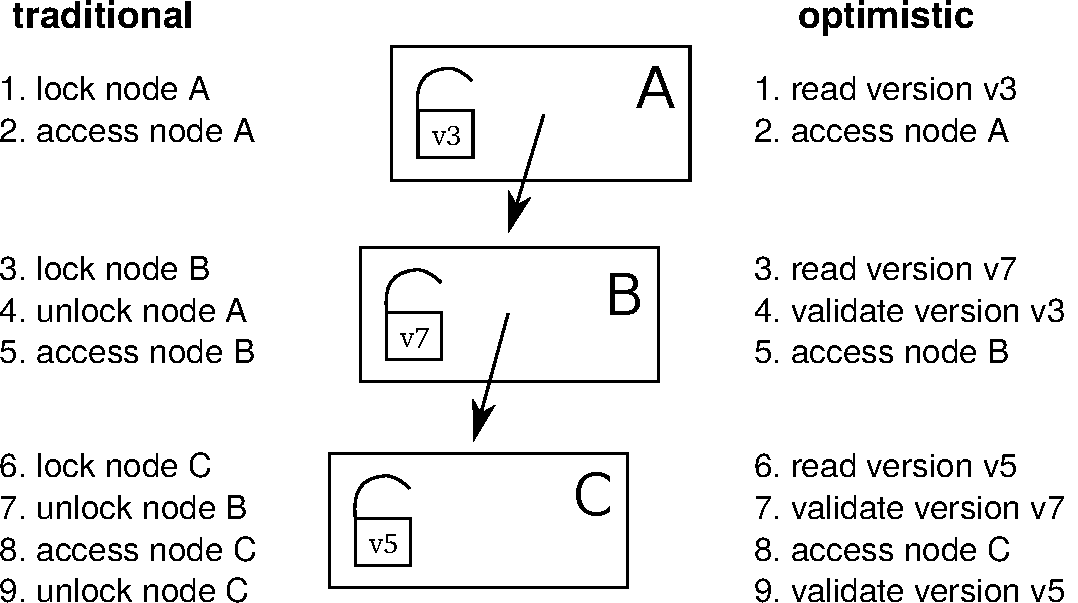
\includegraphics[width=0.65\linewidth]{olcall.pdf}
  \vspace{0.2cm}
  \caption{Comparison of a lookup operation in a 3-level tree using traditional lock coupling (left-hand side) vs.~optimistic lock coupling (right-hand side).}
  \label{fig:olc}
\end{figure}

The traditional and most common lock-based synchronization protocol for B-trees is lock coupling, which interleaves lock acquisitions while holding at most two locks at a time.
If, as we observed earlier, optimistic locks have similar semantics as traditional locks, it is natural to ask whether lock coupling can be combined with optimistic locks.
And indeed the answer is yes: One can almost mechanically translate traditional lock coupling code to optimistic lock coupling code.
This is illustrated in Figure~\ref{fig:olc}, which compares the traversal in a tree of height 3 using traditional and optimistic locks.
As the figure shows, the main difference is that locking is translated to reading the version and that unlocking becomes validation of the previously read version.
This simple change provides efficient lock-free tree traversal without the need to design a complex synchronization protocol.

It is important to emphasize the conceptual simplicity of OLC in comparison to data structures that use custom protocols like the Bw-tree~\cite{DBLP:conf/icde/LevandoskiLS13a}.
To implement lock-free access, the Bw-tree requires an indirection table, delta nodes, complex splitting and merging logic, retry logic, etc.
OLC, on the other hand, can directly be applied to B-trees mostly by adding the appropriate optimistic locking code and without modifying the node layout itself.
Therefore, OpenBw-Tree, an open source implementation of the Bw-tree, requires an order of magnitude more code than a B-tree based on OLC\footnote{Both implementations are available on GitHub: \url{https://github.com/wangziqi2016/index-microbench}}.
Given how difficult it is to develop, validate, and debug lock-free code, simplicity is obviously a major advantage.

\subsection{Correctness Aspects}

\begin{figure}
  % \centering
  %[basicstyle=\normalsize\ttfamily,showstringspaces=false,columns=fullflexible,breaklines=false,breakatwhitespace=true,numbers=none,numberstyle=\small,style=C,keepspaces=true]
\begin{lstlisting}[basicstyle=\ttfamily,language=C++,numbers=left,numberstyle=\small]
std::atomic<BTreeNode*> root;

// search for key in B+tree, returns payload in resultOut
bool lookup(Key key, Value& resultOut) {
   BTreeNode* node = root.load();
   uint64_t nodeVersion = node->readLockOrRestart();
   if (node != root.load()) // make sure the root is still the root
      restart();

   BTreeInner<Key>* parent = nullptr;
   uint64_t parentVersion = 0;

   while (node->isInner()) {
      auto inner = (BTreeInner*)node;

      // unlock parent and make current node the parent
      if (parent)
         parent->readUnlockOrRestart(parentVersion);
      parent = inner;
      parentVersion = nodeVersion;

      // search for next node
      node = inner->findChild(key);
      // validate 'inner' to ensure that 'node' pointer is valid
      inner->checkOrRestart(nodeVersion);
      // now it safe to dereference 'node' pointer (read its version)
      nodeVersion = node->readLockOrRestart();
   }

   // search in leaf and retrieve payload
   auto leaf = (BTreeLeaf*)node;
   bool success = leaf->findValue(key, resultOut);

   // unlock everything
   if (parent)
      parent->readUnlockOrRestart(parentVersion);
   node->readUnlockOrRestart(nodeVersion);

   return success;
}
\end{lstlisting}
  \vspace{0.2cm}
  \caption{B-tree lookup code using OLC. For simplicity, the restart logic is not shown.}
  \label{fig:lookup}
\end{figure}

So far, we have introduced the high-level ideas behind OLC and have stressed its similarity to traditional lock coupling.
Let us now discuss some cases where the close similarity between lock coupling and OLC breaks down.
To make this more concrete, we show the B-tree lookup code in Figure~\ref{fig:lookup}.
In the code, \texttt{readLockOrRestart} reads the lock version and \texttt{readUnlockOrRestart} validates that the read was correct.

One issue with OLC is that any pointer speculatively read from a node may point to invalid memory (if that node is modified concurrently).
Dereferencing such a pointer (e.g., to read its optimistic lock), may cause a segmentation fault or undefined behavior.
In the code shown in Figure~\ref{fig:lookup}, this problem is prevented by the extra check in line 25, which ensures that the read from the node containing the pointer was correct.
Without this additional validation, the code would in line 27 dereference the pointer speculatively read in line 23.
Note that the implementation of \texttt{checkOrRestart} is actually identical to \texttt{readUnlockOrRestart}.
We chose to give it a different name to highlight the fact that this extra check would not be necessary with read/write locks.

Another potential issue with optimistic locks is code that does not terminate.
Code that speculatively accesses a node, like an intra-node binary search, should be written in a way such that it always terminates---even in the presence of concurrent writes.
Otherwise, the validation code that detects the concurrent write will never run.
The binary search of a B-tree, for example, needs to be written in such a way that each comparison makes progress.
For some data structures that do not require loops in the traversal code (like ART) termination is trivially true.

\subsection{Implementation Details}

% implementation, efficiency
To implement an optimistic lock, one can combine the lock and the version counter into a single 64-bit\footnote{Even after subtracting one bit for the lock status, a back-of-the-envelope calculation can show that 63 bits are large enough to never overflow in practice.} word~\cite{artsync}.
A typical read operation will therefore merely consist of reading this version counter atomically.
In C++11 this can be implemented using the \texttt{std::atomic} type.

On x86, atomic reads are cheap because of x86's strong memory order guarantees.
No memory fences are required for sequentially-consistent loads, which are translated (by both GCC and clang) into standard \texttt{MOV} instructions.
Hence, the only effect of \texttt{std::atomic} for loads is preventing instruction re-ordering.
This makes version access and validation cheap.
Acquiring and releasing an optimistic lock in exclusive mode has comparable cost to a traditional lock:
A fairly expensive sequentially-consistent store is needed for acquiring a lock, while a standard \texttt{MOV} suffices for releasing it.
A simple sinlock-based implementation of optimistic locks can be found in the appendix of an earlier paper~\cite{artsync}.

OLC code must be able to handle restarts since validation or lock upgrade can fail due to concurrent writers.
Restarts can easily be implemented by wrapping the data structure operation in a loop (for simplicity not shown in Figure~\ref{fig:lookup}).
Such a loop also enables limiting the number of optimistic retry operations and falling back to pessimistic locking in cases of very heavy contention.
The ability to fall back to traditional locking is a major advantage of OLC in terms of robustness over lock-free approaches, which do not have this option.

In addition to the optimistic shared mode and the exclusive mode, optimistic locks also support a ``shared pessimistic'' mode, which physically acquires the lock in shared mode (allowing multiple concurrent readers but no writers).
This mode is useful for table (or range) scans that touch many tuples on a leaf page (which would otherwise easily abort).
Finally, let us mention that large range scans and table scans, should be broken up into several per-node traversals as is done in the LeanStore~\cite{leanstore} system.

Like all lock-free data structures, but unlike traditional locking and Hardware Transactional Memory~\cite{DBLP:conf/hpca/KarnagelDRLLSL14,DBLP:journals/pvldb/MakreshanskiLS15,htmtkde}, OLC requires care when deleting (and reusing) nodes.
The reason is that a deleting thread can never be sure that a node can be reclaimed because other threads might still be optimistically reading from that node.
Therefore, standard solutions like epoch-based reclamation~\cite{DBLP:conf/sosp/TuZKLM13}, hazard pointers~\cite{DBLP:journals/tpds/Michael04}, or optimized hazard pointers~\cite{DBLP:conf/spaa/BalmauGHZ16} need to be used.
These memory reclamation techniques are, however, largely orthogonal to the synchronization protocol itself.

%-lock-free is not a strong guarantee

\newpage
\section{Evaluation}\label{sec:evaluation}

Let us now experimentally evaluate the overhead and scalability of OLC.
For the experiments, we use an in-memory B+tree implemented in C++11 using templates, which is configured to use nodes of 4096 bytes, random 8 byte keys, and 8 byte payloads.
Based on this B-tree, we compare the following synchronization approaches:
\begin{itemize}
\item an OLC implementation\footnote{An almost identical OLC implementation is available on github: \url{https://github.com/wangziqi2016/index-microbench/tree/master/BTreeOLC}}
\item a variant based on traditional lock coupling and read/write locks
\item the unsynchronized B-tree, which obviously is only correct for read-only workloads but allows measuring the overhead of synchronization
\end{itemize}
Note that earlier work has compared the OLC implementation with a Bw-tree implementation~\cite{buzzword} and other state-of-the-art in-memory index structures.

We use a Haswell EP system with an Intel Xeon E5-2687W v3 CPU, which has 10 cores (20 ``Hyper-Threads'') and 25~MB of L3 cache.
The system is running Ubuntu 18.10 and we use GCC 8.2.0 to compile our code.
The CPU counters are obtained using the Linux perf API\footnote{We use the following convenience wrapper: \url{https://github.com/viktorleis/perfevent}}.

\begin{table}
  \caption{Performance and CPU counters for lookup and insert operations in a B-tree with 100M keys. We perform 100M operations and normalize the CPU counters by that number.}
  \label{tab:overhead}
  \centering
  \begin{tabular}{lrrrrrrr}\toprule
                    &         &        &        & instruc-  & L1     & L3     & branch \\
                    & threads & M op/s & cycles & tions & misses & misses & misses \\\midrule
lookup (no sync.)   & 1       & 1.72   & 2028   & 283     & 39.1   & 14.9   & 16.1   \\
lookup (OLC)        & 1       & 1.65   & 2107   & 370     & 43.9   & 15.1   & 16.7   \\
lookup (lock coup.) & 1       & 1.72   & 2078   & 365     & 42.3   & 16.9   & 15.7   \\\midrule
insert (no sync.)   & 1       & 1.51   & 2286   & 530     & 59.8   & 31.1   & 17.3   \\
insert (OLC)        & 1       & 1.50   & 2303   & 629     & 61.2   & 31.1   & 16.5   \\
insert (lock coup.) & 1       & 1.41   & 2473   & 644     & 61.0   & 31.0   & 17.2   \\\midrule
lookup (no sync.)   & 10      & 15.48  & 2058   & 283     & 38.6   & 15.5   & 16.0   \\
lookup (OLC)        & 10      & 14.60  & 2187   & 370     & 43.8   & 15.8   & 16.8   \\
lookup (lock coup.) & 10      & 5.71   & 5591   & 379     & 54.2   & 17.0   & 14.8   \\\midrule
insert (no sync.)   & 10      & -      & -      & -       & -      & -      & -      \\
insert (OLC)        & 10      & 10.46  & 2940   & 656     & 62.0   & 32.5   & 16.8   \\
insert (lock coup.) & 10      & 7.55   & 4161   & 667     & 75.0   & 28.6   & 16.2   \\
    \bottomrule
\end{tabular}
\end{table}

Table~\ref{tab:overhead} compares the performance and CPU counters for lookup and insert operations in a B-tree with 100M keys.
With {\em single-threaded} execution, we observe that all three approaches have very similar performance.
Adding traditional or optimistic locks to unsynchronized B-tree code results in up to 30\% of additional instructions without affecting single-threaded performance much.

\begin{figure}
  \centering
  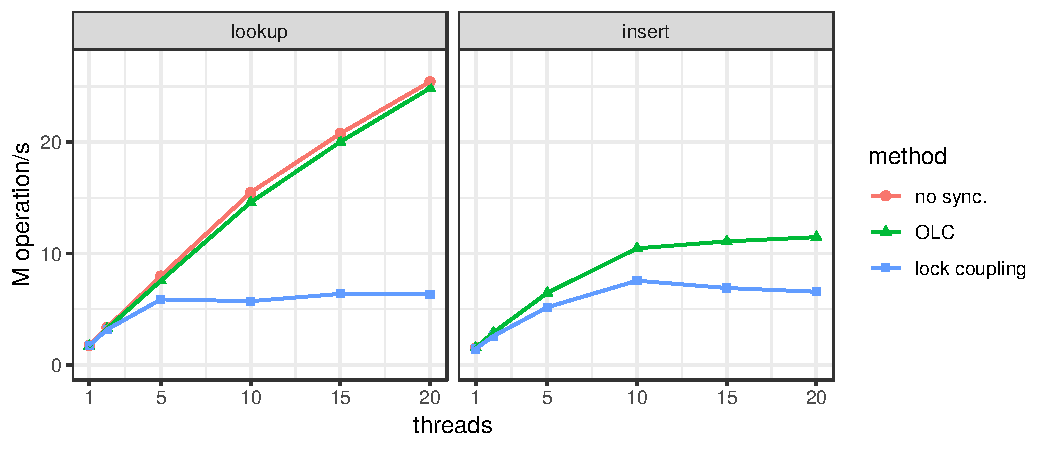
\includegraphics[width=\linewidth]{scale.pdf}
  \vspace{0.2cm}
  \caption{Scalability on 10-core system for B-tree operations (100M values).}
  \label{fig:scale}
\end{figure}

As Figure~\ref{fig:scale} shows, the results change dramatically once we use multiple threads.
For lookup, the scalability of OLC is near-linear up to 20 threads, even though the system has only 10 ``real cores''.
The OLC scalability for insert is also respectable (though not quite as linear because multi-threaded insertion approaches the memory bandwidth of our processor).
The figure also shows that the results of traditional lock coupling with read/write locks are significantly worse than OLC.
With 20 threads, lookup with OLC is 3.9$\times$ faster than traditional lock coupling.

\section{Summary}\label{sec:conc}

Optimistic Lock Coupling (OLC) is an effective synchronization method that combines the simplicity of traditional lock coupling with the superior scalability of lock-free approaches.
OLC is widely applicable and has already been successfully used to synchronize several data structures, including B-trees, binary search trees, and different trie variants.
These features make it highly attractive for modern database systems as well as performance-critical systems software in general.

\begin{thebibliography}{10}

\bibitem{DBLP:conf/spaa/BalmauGHZ16}
O.~Balmau, R.~Guerraoui, M.~Herlihy, and I.~Zablotchi.
\newblock Fast and robust memory reclamation for concurrent data structures.
\newblock In {\em SPAA}, 2016.

\bibitem{DBLP:journals/acta/BayerS77}
R.~Bayer and M.~Schkolnick.
\newblock Concurrency of operations on {B}-trees.
\newblock {\em Acta Informatica}, 9, 1977.

\bibitem{hot}
R.~Binna, E.~Zangerle, M.~Pichl, G.~Specht, and V.~Leis.
\newblock {HOT}: A height optimized trie index for main-memory database
  systems.
\newblock In {\em SIGMOD}, 2018.

\bibitem{DBLP:conf/ppopp/BronsonCCO10}
N.~G. Bronson, J.~Casper, H.~Chafi, and K.~Olukotun.
\newblock A practical concurrent binary search tree.
\newblock In {\em PPOPP}, 2010.

\bibitem{DBLP:conf/vldb/ChaHKK01}
S.~K. Cha, S.~Hwang, K.~Kim, and K.~Kwon.
\newblock Cache-conscious concurrency control of main-memory indexes on
  shared-memory multiprocessor systems.
\newblock In {\em VLDB}, 2001.

\bibitem{intel}
I.~Cutress.
\newblock {Intel} goes for 48-cores: {Cascade-AP} with multi-chip package
  coming soon.
\newblock
  \url{https://www.anandtech.com/show/13535/intel-goes-for-48cores-cascade-ap},
  2018 (accessed January, 2019).

\bibitem{DBLP:conf/cidr/FaleiroA17}
J.~M. Faleiro and D.~J. Abadi.
\newblock Latch-free synchronization in database systems: Silver bullet or
  fool's gold?
\newblock In {\em CIDR}, 2017.

\bibitem{DBLP:journals/ftdb/Graefe11}
G.~Graefe.
\newblock Modern {B}-tree techniques.
\newblock {\em Foundations and Trends in Databases}, 3(4), 2011.

\bibitem{DBLP:conf/hpca/KarnagelDRLLSL14}
T.~Karnagel, R.~Dementiev, R.~Rajwar, K.~Lai, T.~Legler, B.~Schlegel, and
  W.~Lehner.
\newblock Improving in-memory database index performance with
  {Intel}\({}^{\mbox{{\textregistered}}}\) transactional synchronization
  extensions.
\newblock In {\em HPCA}, 2014.

\bibitem{DBLP:journals/tods/LehmanY81}
P.~L. Lehman and S.~B. Yao.
\newblock Efficient locking for concurrent operations on {B}-trees.
\newblock {\em {ACM} Trans. Database Syst.}, 6(4), 1981.

\bibitem{leanstore}
V.~Leis, M.~Haubenschild, A.~Kemper, and T.~Neumann.
\newblock Leanstore: In-memory data management beyond main memory.
\newblock In {\em ICDE}, 2018.

\bibitem{art}
V.~Leis, A.~Kemper, and T.~Neumann.
\newblock The adaptive radix tree: {ARTful} indexing for main-memory databases.
\newblock In {\em ICDE}, 2013.

\bibitem{htmtkde}
V.~Leis, A.~Kemper, and T.~Neumann.
\newblock Scaling {HTM}-supported database transactions to many cores.
\newblock {\em {IEEE} Trans. Knowl. Data Eng.}, 28(2), 2016.

\bibitem{artsync}
V.~Leis, F.~Scheibner, A.~Kemper, and T.~Neumann.
\newblock The {ART} of practical synchronization.
\newblock In {\em DaMoN}, 2016.

\bibitem{DBLP:conf/icde/LevandoskiLS13a}
J.~J. Levandoski, D.~B. Lomet, and S.~Sengupta.
\newblock The {Bw}-tree: A {B}-tree for new hardware platforms.
\newblock In {\em ICDE}, 2013.

\bibitem{DBLP:journals/pvldb/MakreshanskiLS15}
D.~Makreshanski, J.~J. Levandoski, and R.~Stutsman.
\newblock To lock, swap, or elide: On the interplay of hardware transactional
  memory and lock-free indexing.
\newblock {\em {PVLDB}}, 8(11), 2015.

\bibitem{DBLP:dblp_conf/eurosys/MaoKM12}
Y.~Mao, E.~Kohler, and R.~T. Morris.
\newblock Cache craftiness for fast multicore key-value storage.
\newblock In {\em EuroSys}, 2012.

\bibitem{DBLP:journals/tpds/Michael04}
M.~M. Michael.
\newblock Hazard pointers: Safe memory reclamation for lock-free objects.
\newblock {\em {IEEE} Trans. Parallel Distrib. Syst.}, 15(6), 2004.

\bibitem{DBLP:journals/jacm/ShalevS06}
O.~Shalev and N.~Shavit.
\newblock Split-ordered lists: Lock-free extensible hash tables.
\newblock {\em J. {ACM}}, 53(3), 2006.

\bibitem{amd}
A.~Shilov.
\newblock {AMD} previews {EPYC} ‘{Rome}’ processor: Up to 64 {Zen} 2 cores.
\newblock
  \url{https://www.anandtech.com/show/13561/amd-previews-epyc-rome-processor-up-to-64-zen-2-cores},
  2018 (accessed January, 2019).

\bibitem{DBLP:conf/sosp/TuZKLM13}
S.~Tu, W.~Zheng, E.~Kohler, B.~Liskov, and S.~Madden.
\newblock Speedy transactions in multicore in-memory databases.
\newblock In {\em SOSP}, 2013.

\bibitem{buzzword}
Z.~Wang, A.~Pavlo, H.~Lim, V.~Leis, H.~Zhang, M.~Kaminsky, and D.~Andersen.
\newblock Building a {Bw}-tree takes more than just buzz words.
\newblock In {\em SIGMOD}, 2018.

\end{thebibliography}


%\bibliographystyle{abbrv}
%\bibliography{main}

\end{document}

\end{article}


\begin{article}
{Hypergraph Clustering Network for Interaction Data}
{Tianchi Yang, Luhao Zhang, Cheng Yang, Chuan Shi, Maodi Hu, Tao Li, and Dong Wang}
\pdfminorversion=5
\documentclass[11pt]{article}
\usepackage{deauthor,times,graphicx,caption,microtype}
\usepackage{hyperref}
\usepackage{listings}
\usepackage{booktabs}

\begin{document}

\title{Optimistic Lock Coupling: A Scalable and Efficient General-Purpose Synchronization Method}

\author{Viktor Leis, Michael Haubenschild\raisebox{0.9ex}{$\ast$}, Thomas Neumann\\ Technische Universit{\"a}t M{\"u}nchen \hspace{0.7cm} Tableau Software\raisebox{0.9ex}{$\ast$} \\ {\{leis,neumann\}{@}in.tum.de} \hspace{0.7cm} {mhaubenschild{@}tableau.com\raisebox{0.9ex}{$\ast$}}}

\maketitle

\begin{abstract}
As the number of cores on commodity processors continues to increase, scalability becomes more and more crucial for overall performance.
Scalable and efficient concurrent data structures are particularly important, as these are often the building blocks of parallel algorithms.
Unfortunately, traditional synchronization techniques based on fine-grained locking have been shown to be unscalable on modern multi-core CPUs.
Lock-free data structures, on the other hand, are extremely difficult to design and often incur significant overhead.

In this work, we make the case for Optimistic Lock Coupling as a practical alternative to both traditional locking and the lock-free approach.
We show that Optimistic Lock Coupling is highly scalable and almost as simple to implement as traditional lock coupling.
Another important advantage is that it is easily applicable to most tree-like data structures.
We therefore argue that Optimistic Lock Coupling, rather than a complex and error-prone custom synchronization protocol, should be the default choice for performance-critical data structures.
\end{abstract}

\section{Introduction}

% more and more cores
Today, Intel's commodity server processors have up to 28 cores and its upcoming microarchitecture will have up to 48 cores per socket~\cite{intel}.
Similarly, AMD currently stands at 32 cores and this number is expected to double in the next generation~\cite{amd}.
Since both platforms support simultaneous multithreading (also known as hyperthreading), affordable commodity servers (with up to two sockets) will soon routinely have between 100 and 200 hardware threads.

% data structure scalability is important
With such a high degree of hardware parallelism, efficient data processing crucially depends on how well concurrent data structures scale.
Internally, database systems use a plethora of data structures like table heaps, internal work queues, and, most importantly, index structures.
Any of these can easily become a scalability (and therefore overall performance) bottleneck on many-core CPUs.

% traditional synchronization: fine-grained locks, slow, cache invalidation
Traditionally, database systems synchronize internal data structures using fine-grained reader/writer locks\footnote{In this work, we focus on data structure synchronization rather than high-level transaction semantics and therefore use the term {\em lock} for what would typically be called {\em latch} in the database literature. We thus follow common computer science (rather than database) terminology.}.
Unfortunately, while fine-grained locking makes lock contention unlikely, it still results in bad scalability because lock acquisition and release require writing to shared memory.
Due to the way cache coherency is implemented on modern multi-core CPUs, these writes cause additional cache misses\footnote{The cache coherency protocol ensures that all copies of a cache line on other cores are invalidated before the write can proceed.} and the cache line containing the lock's internal data becomes a point of physical contention.
As a result, any frequently-accessed lock (e.g., the lock of the root node of a B-tree) severely limits scalability.

% lock-free bw-tree: no more latches, but indirections, extremely complex
Lock-free data structures like the Bw-tree~\cite{DBLP:conf/icde/LevandoskiLS13a} (a lock-free B-tree variant) or the Split-Ordered List~\cite{DBLP:journals/jacm/ShalevS06} (a lock-free hash table) do not acquire any locks and therefore generally scale much better than locking-based approaches (in particular for read-mostly workloads).
However, lock-free synchronization has other downsides:
First, it is very difficult and results in extremely complex and error-prone code (when compared to locking).
Second, because the functionality of atomic primitives provided by the hardware (e.g., atomically compare-and-swap 8 bytes) is limited, complex operations require additional indirections within the data structure.
For example, the Bw-tree requires an indirection table and the Split-Ordered List requires ``dummy nodes'', resulting in overhead due to additional cache misses.

% OLC for the win
In this paper we make the case for {\em Optimistic Lock Coupling (OLC)}, a synchronization method that combines some of the best properties of lock-based and lock-free synchronization.
OLC utilizes a special lock type that can be used in two modes:
The first mode is similar to a traditional mutex and excludes other threads by physically acquiring the underlying lock.
In the second mode, reads can proceed optimistically by validating a version counter that is embedded in the lock (similar to optimistic concurrency control).
The first mode is typically used by writers and the second mode by readers.
Besides this special lock type, OLC is based on the observation that optimistic lock validations can be interleaved/coupled---similar to the pair-wise interleaved lock acquisition of traditional lock coupling.
Hence, the name Optimistic Lock Coupling.

OLC has a number of desirable features:
\begin{itemize}
\item By reducing the number of writes to shared memory locations and thereby avoiding cache invalidations, it {\bf scales well} for most workloads.
\item In comparison to unsynchronized code, it requires few additional CPU instructions making it {\bf efficient}.
\item OLC is {\bf widely applicable} to different data structures. It has already been successfully used for synchronizing binary search trees~\cite{DBLP:conf/ppopp/BronsonCCO10}, tries~\cite{artsync}, trie/B-tree hybrids~\cite{DBLP:dblp_conf/eurosys/MaoKM12}, and B-trees~\cite{buzzword}.
\item In comparison to the lock-free paradigm, it is also {\bf easy to use} and requires few modifications to existing, single-threaded data structures.
\end{itemize}
Despite these positive features and its simplicity, OLC is not yet widely known.
The goal of this paper is therefore to popularize this simple idea and to make a case for it.
We argue that OLC deserves to be widely known.
It is a good default synchronization paradigm---more complex, data structure-specific protocols are seldom beneficial.

The rest of the paper is organized as follows.
Section~\ref{sec:related} discusses related work, tracing the history of OLC and its underlying ideas in the literature.
The core of the paper is Section~\ref{sec:olc}, which describes the ideas behind OLC and how it can be used to synchronize complex data structures.
In Section~\ref{sec:evaluation} we experimentally show that OLC has low overhead and scales well when used to synchronize an in-memory B-tree.
We summarize the paper in Section~\ref{sec:conc}.

\newpage
\section{Related Work}\label{sec:related}

Lock coupling has been proposed as a method for allowing concurrent operations on B-trees in 1977~\cite{DBLP:journals/acta/BayerS77}.
This traditional and still widely-used method, described in detail in Graefe's B-tree survey~\cite{DBLP:journals/ftdb/Graefe11}, is also called ``latch coupling'', ``hand-over-hand locking'', and ``crabbing''.
Because at most two locks are held at-a-time during tree traversal, this technique seemingly allows for a high degree of parallelism---in particular if read/write locks are used to enable inner nodes to be locked in shared mode.
However, as we show in Section~\ref{sec:evaluation}, on modern hardware lock acquisition (even in shared mode) results in suboptimal scalability.

An early alternative from 1981 is a B-tree variant called B-link tree~\cite{DBLP:journals/tods/LehmanY81}, which only holds a single lock at a time.
It is based on the observation that between the release of the parent lock and the acquisition of the child lock, the only ``dangerous'' thing that could have happened is the split of a child node (assuming one does not implement merge operations).
Thus, when a split happens, the key being searched might end up on a neighboring node to the right of the current child node.
A B-link tree traversal therefore detects this condition and, if needed, transparently proceeds to the neighboring node.
Releasing the parent lock early is highly beneficial when the child node needs to be fetched from disk.
For in-memory workloads, however, the B-link tree has the same scalability issues as lock coupling (it acquires just as many locks).

The next major advance, Optimistic Latch-Free Index Traversal (OLFIT)~\cite{DBLP:conf/vldb/ChaHKK01}, was proposed in 2001.
OLFIT introduced the idea of a combined lock/update counter, which we call {\em optimistic lock}. % , for lack of a better name,
Based on these per-node optimistic locks and the synchronization protocol of the B-link tree, OLFIT finally achieves good scalability on parallel processors.
The OLFIT protocol is fairly complex, as it requires both the non-trivial B-link protocol and optimistic locks.
Furthermore, like the B-link tree protocol, it does not support merging nodes, and is specific to B-trees (cannot easily be applied to other data structures).

In the following two decades, the growth of main-memory capacity led to much research into other data structures besides the venerable B-tree.
Particularly relevant for our discussion is Bronson et al.'s~\cite{DBLP:conf/ppopp/BronsonCCO10} concurrent binary search tree, which is based on optimistic version validation and has a sophisticated, data structure-specific synchronization protocol.
To the best of our knowledge, this 2010 paper is the first that, as part of its protocol, interleaves version validation across nodes---rather than validating each node separately like OLFIT.
In that paper, this idea is called ``hand-over-hand, optimistic validation'', while we prefer the term Optimistic Lock Coupling to highlight the close resemblance to traditional lock coupling.
Similarly, Mao et al.'s~\cite{DBLP:dblp_conf/eurosys/MaoKM12} Masstree (a concurrent hybrid trie/B-tree) is also based on the same ideas, but again uses them as part of a more complex protocol.

The Adaptive Radix Tree (ART)~\cite{art} is another recent in-memory data structure, which we proposed in 2013.
In contrast to the two data structures just mentioned, it was originally designed with single-threaded performance in mind without supporting concurrency.
To add support for concurrency, we initially started designing a custom protocol called Read-Optimized Write Exclusion (ROWEX)~\cite{artsync}, which turned out to be non-trivial and requires modifications of the underlying data structure\footnote{Note that ROWEX is already easier to apply to existing data structures than the lock-free approach. The difficulty depends on the data structure. Applying ROWEX is hard for B-trees with sorted keys and fairly easy for copy-on-write data structures like the Height Optimized Trie~\cite{hot}---with ART being somewhere in the middle.}.
However, fairly late in the project, we also realized, that OLC {\em alone} (rather than as part of a more complex protocol) is sufficient to synchronize ART.
No other changes to the data structure were necessary.
Both approaches were published and experimentally evaluated in a followup paper~\cite{artsync}, which shows that, despite its simplicity, OLC is efficient, scalable, and generally outperforms ROWEX.

Similar results were recently published regarding B-trees~\cite{buzzword}.
In this experimental study a simple OLC-based synchronization outperformed the Bw-tree~\cite{DBLP:conf/icde/LevandoskiLS13a}, a complex lock-free synchronization approach.
Another recent paper shows that for write-intensive workloads, locking often performs better than lock-free synchronization~\cite{DBLP:conf/cidr/FaleiroA17}.
These experiences indicate that OLC is a general-purpose synchronization paradigm and motivate the current paper.

%foster b-tree\cite{DBLP:journals/tods/GraefeKK12}
%Shasha theory~\cite{DBLP:journals/tods/ShashaG88}

\section{Optimistic Lock Coupling}\label{sec:olc}

% locks suck
The standard technique for inter-thread synchronization is mutual exclusion using fine-grained locks.
In a B-tree, for example, every node usually has its own associated lock, which is acquired before accessing that node.
The problem of locking on modern multi- and many-core processors is that lock acquisition and release require writing to the shared memory location that implements the lock.
This write causes exclusive ownership of the underlying cache line and invalidates copies of it on all other processor cores.
For hierarchical, tree-like data structures, the lock of the root node becomes a point of physical contention---even in read-only workloads and even when read/write locks are used.
Depending on the specific data structure, number of cores, cache coherency protocol implementation, cache topology, whether Non-Uniform Memory Access (NUMA) is used, locking can even result in multi-threaded performance that is worse than single-threaded execution.

% in b-trees this happens very much
The inherent pessimism of locking is particularly unfortunate for B-trees:
Despite the fact that logical modifications of the root node are very infrequent, every B-tree operation must lock the root node during tree traversal\footnote{To a lesser extent this obviously applies to all inner nodes, not just the root.}.
Even the vast majority of update operations (with the exception of splits and merges), only modify a single leaf node.
These observations indicate that a more optimistic approach, which does not require locking inner nodes, would be very beneficial for B-trees.

\subsection{Optimistic Locks}

% optimism to the rescue
As the name indicates, optimistic locks try to solve the scalability issues of traditional locks using an optimistic approach.
Instead of always physically acquiring locks, even for nodes that are unlikely to be modified simultaneously, after-the-fact validation is used to detect conflicts.
This is done by augmenting each lock with a version/update counter that is incremented on every modification.
Using this version counter, readers can optimistically proceed before validating that the version did not change to ensure that the read was safe.
If validation fails, the operation is restarted.

% details on opt locks
Using optimistic locks, a read-only node access (i.e., the majority of all operations in a B-tree) does not acquire the lock and does not increment the version counter.
Instead, it performs the following steps:
\begin{enumerate}
\item read lock version (restart if lock is not free)
\item access node
\item read the version again and validate that it has not changed in the meantime
\end{enumerate}
If the last step (the validation) fails, the operation has to be restarted.
Write operations, on the other hand, are more similar to traditional locking:
\begin{enumerate}
\item acquire lock (wait if necessary)
\item access/write to node
\item increment version and unlock node
\end{enumerate}
Writes can therefore protect a node from other writes.

% similar to locks
As we observed in an earlier paper~\cite{artsync}, because of similar semantics, optimistic locks can be hidden behind an API very similar to traditional read/write locks.
Both approaches have an exclusive lock mode, and acquiring a traditional lock in shared mode is analogous to optimistic version validation.
Furthermore, like with some implementations of traditional read/write locks, optimistic locks allow upgrading a shared lock to an exclusive lock.
Lock upgrades are, for example, used to avoid most B-tree update operations from having to lock inner nodes.
In our experience, the close resemblance of optimistic and traditional locks simplifies the reasoning about optimistic locks;
one can apply similar thinking as in traditional lock-based protocols.

\subsection{Lock Coupling with Optimistic Locks}

\begin{figure}
  \centering
  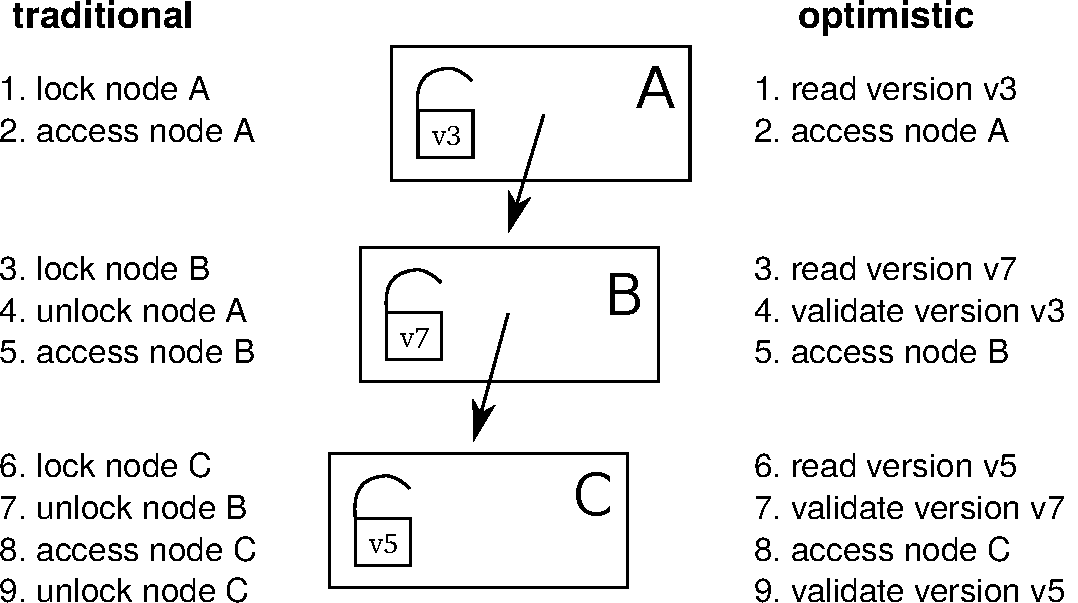
\includegraphics[width=0.65\linewidth]{olcall.pdf}
  \vspace{0.2cm}
  \caption{Comparison of a lookup operation in a 3-level tree using traditional lock coupling (left-hand side) vs.~optimistic lock coupling (right-hand side).}
  \label{fig:olc}
\end{figure}

The traditional and most common lock-based synchronization protocol for B-trees is lock coupling, which interleaves lock acquisitions while holding at most two locks at a time.
If, as we observed earlier, optimistic locks have similar semantics as traditional locks, it is natural to ask whether lock coupling can be combined with optimistic locks.
And indeed the answer is yes: One can almost mechanically translate traditional lock coupling code to optimistic lock coupling code.
This is illustrated in Figure~\ref{fig:olc}, which compares the traversal in a tree of height 3 using traditional and optimistic locks.
As the figure shows, the main difference is that locking is translated to reading the version and that unlocking becomes validation of the previously read version.
This simple change provides efficient lock-free tree traversal without the need to design a complex synchronization protocol.

It is important to emphasize the conceptual simplicity of OLC in comparison to data structures that use custom protocols like the Bw-tree~\cite{DBLP:conf/icde/LevandoskiLS13a}.
To implement lock-free access, the Bw-tree requires an indirection table, delta nodes, complex splitting and merging logic, retry logic, etc.
OLC, on the other hand, can directly be applied to B-trees mostly by adding the appropriate optimistic locking code and without modifying the node layout itself.
Therefore, OpenBw-Tree, an open source implementation of the Bw-tree, requires an order of magnitude more code than a B-tree based on OLC\footnote{Both implementations are available on GitHub: \url{https://github.com/wangziqi2016/index-microbench}}.
Given how difficult it is to develop, validate, and debug lock-free code, simplicity is obviously a major advantage.

\subsection{Correctness Aspects}

\begin{figure}
  % \centering
  %[basicstyle=\normalsize\ttfamily,showstringspaces=false,columns=fullflexible,breaklines=false,breakatwhitespace=true,numbers=none,numberstyle=\small,style=C,keepspaces=true]
\begin{lstlisting}[basicstyle=\ttfamily,language=C++,numbers=left,numberstyle=\small]
std::atomic<BTreeNode*> root;

// search for key in B+tree, returns payload in resultOut
bool lookup(Key key, Value& resultOut) {
   BTreeNode* node = root.load();
   uint64_t nodeVersion = node->readLockOrRestart();
   if (node != root.load()) // make sure the root is still the root
      restart();

   BTreeInner<Key>* parent = nullptr;
   uint64_t parentVersion = 0;

   while (node->isInner()) {
      auto inner = (BTreeInner*)node;

      // unlock parent and make current node the parent
      if (parent)
         parent->readUnlockOrRestart(parentVersion);
      parent = inner;
      parentVersion = nodeVersion;

      // search for next node
      node = inner->findChild(key);
      // validate 'inner' to ensure that 'node' pointer is valid
      inner->checkOrRestart(nodeVersion);
      // now it safe to dereference 'node' pointer (read its version)
      nodeVersion = node->readLockOrRestart();
   }

   // search in leaf and retrieve payload
   auto leaf = (BTreeLeaf*)node;
   bool success = leaf->findValue(key, resultOut);

   // unlock everything
   if (parent)
      parent->readUnlockOrRestart(parentVersion);
   node->readUnlockOrRestart(nodeVersion);

   return success;
}
\end{lstlisting}
  \vspace{0.2cm}
  \caption{B-tree lookup code using OLC. For simplicity, the restart logic is not shown.}
  \label{fig:lookup}
\end{figure}

So far, we have introduced the high-level ideas behind OLC and have stressed its similarity to traditional lock coupling.
Let us now discuss some cases where the close similarity between lock coupling and OLC breaks down.
To make this more concrete, we show the B-tree lookup code in Figure~\ref{fig:lookup}.
In the code, \texttt{readLockOrRestart} reads the lock version and \texttt{readUnlockOrRestart} validates that the read was correct.

One issue with OLC is that any pointer speculatively read from a node may point to invalid memory (if that node is modified concurrently).
Dereferencing such a pointer (e.g., to read its optimistic lock), may cause a segmentation fault or undefined behavior.
In the code shown in Figure~\ref{fig:lookup}, this problem is prevented by the extra check in line 25, which ensures that the read from the node containing the pointer was correct.
Without this additional validation, the code would in line 27 dereference the pointer speculatively read in line 23.
Note that the implementation of \texttt{checkOrRestart} is actually identical to \texttt{readUnlockOrRestart}.
We chose to give it a different name to highlight the fact that this extra check would not be necessary with read/write locks.

Another potential issue with optimistic locks is code that does not terminate.
Code that speculatively accesses a node, like an intra-node binary search, should be written in a way such that it always terminates---even in the presence of concurrent writes.
Otherwise, the validation code that detects the concurrent write will never run.
The binary search of a B-tree, for example, needs to be written in such a way that each comparison makes progress.
For some data structures that do not require loops in the traversal code (like ART) termination is trivially true.

\subsection{Implementation Details}

% implementation, efficiency
To implement an optimistic lock, one can combine the lock and the version counter into a single 64-bit\footnote{Even after subtracting one bit for the lock status, a back-of-the-envelope calculation can show that 63 bits are large enough to never overflow in practice.} word~\cite{artsync}.
A typical read operation will therefore merely consist of reading this version counter atomically.
In C++11 this can be implemented using the \texttt{std::atomic} type.

On x86, atomic reads are cheap because of x86's strong memory order guarantees.
No memory fences are required for sequentially-consistent loads, which are translated (by both GCC and clang) into standard \texttt{MOV} instructions.
Hence, the only effect of \texttt{std::atomic} for loads is preventing instruction re-ordering.
This makes version access and validation cheap.
Acquiring and releasing an optimistic lock in exclusive mode has comparable cost to a traditional lock:
A fairly expensive sequentially-consistent store is needed for acquiring a lock, while a standard \texttt{MOV} suffices for releasing it.
A simple sinlock-based implementation of optimistic locks can be found in the appendix of an earlier paper~\cite{artsync}.

OLC code must be able to handle restarts since validation or lock upgrade can fail due to concurrent writers.
Restarts can easily be implemented by wrapping the data structure operation in a loop (for simplicity not shown in Figure~\ref{fig:lookup}).
Such a loop also enables limiting the number of optimistic retry operations and falling back to pessimistic locking in cases of very heavy contention.
The ability to fall back to traditional locking is a major advantage of OLC in terms of robustness over lock-free approaches, which do not have this option.

In addition to the optimistic shared mode and the exclusive mode, optimistic locks also support a ``shared pessimistic'' mode, which physically acquires the lock in shared mode (allowing multiple concurrent readers but no writers).
This mode is useful for table (or range) scans that touch many tuples on a leaf page (which would otherwise easily abort).
Finally, let us mention that large range scans and table scans, should be broken up into several per-node traversals as is done in the LeanStore~\cite{leanstore} system.

Like all lock-free data structures, but unlike traditional locking and Hardware Transactional Memory~\cite{DBLP:conf/hpca/KarnagelDRLLSL14,DBLP:journals/pvldb/MakreshanskiLS15,htmtkde}, OLC requires care when deleting (and reusing) nodes.
The reason is that a deleting thread can never be sure that a node can be reclaimed because other threads might still be optimistically reading from that node.
Therefore, standard solutions like epoch-based reclamation~\cite{DBLP:conf/sosp/TuZKLM13}, hazard pointers~\cite{DBLP:journals/tpds/Michael04}, or optimized hazard pointers~\cite{DBLP:conf/spaa/BalmauGHZ16} need to be used.
These memory reclamation techniques are, however, largely orthogonal to the synchronization protocol itself.

%-lock-free is not a strong guarantee

\newpage
\section{Evaluation}\label{sec:evaluation}

Let us now experimentally evaluate the overhead and scalability of OLC.
For the experiments, we use an in-memory B+tree implemented in C++11 using templates, which is configured to use nodes of 4096 bytes, random 8 byte keys, and 8 byte payloads.
Based on this B-tree, we compare the following synchronization approaches:
\begin{itemize}
\item an OLC implementation\footnote{An almost identical OLC implementation is available on github: \url{https://github.com/wangziqi2016/index-microbench/tree/master/BTreeOLC}}
\item a variant based on traditional lock coupling and read/write locks
\item the unsynchronized B-tree, which obviously is only correct for read-only workloads but allows measuring the overhead of synchronization
\end{itemize}
Note that earlier work has compared the OLC implementation with a Bw-tree implementation~\cite{buzzword} and other state-of-the-art in-memory index structures.

We use a Haswell EP system with an Intel Xeon E5-2687W v3 CPU, which has 10 cores (20 ``Hyper-Threads'') and 25~MB of L3 cache.
The system is running Ubuntu 18.10 and we use GCC 8.2.0 to compile our code.
The CPU counters are obtained using the Linux perf API\footnote{We use the following convenience wrapper: \url{https://github.com/viktorleis/perfevent}}.

\begin{table}
  \caption{Performance and CPU counters for lookup and insert operations in a B-tree with 100M keys. We perform 100M operations and normalize the CPU counters by that number.}
  \label{tab:overhead}
  \centering
  \begin{tabular}{lrrrrrrr}\toprule
                    &         &        &        & instruc-  & L1     & L3     & branch \\
                    & threads & M op/s & cycles & tions & misses & misses & misses \\\midrule
lookup (no sync.)   & 1       & 1.72   & 2028   & 283     & 39.1   & 14.9   & 16.1   \\
lookup (OLC)        & 1       & 1.65   & 2107   & 370     & 43.9   & 15.1   & 16.7   \\
lookup (lock coup.) & 1       & 1.72   & 2078   & 365     & 42.3   & 16.9   & 15.7   \\\midrule
insert (no sync.)   & 1       & 1.51   & 2286   & 530     & 59.8   & 31.1   & 17.3   \\
insert (OLC)        & 1       & 1.50   & 2303   & 629     & 61.2   & 31.1   & 16.5   \\
insert (lock coup.) & 1       & 1.41   & 2473   & 644     & 61.0   & 31.0   & 17.2   \\\midrule
lookup (no sync.)   & 10      & 15.48  & 2058   & 283     & 38.6   & 15.5   & 16.0   \\
lookup (OLC)        & 10      & 14.60  & 2187   & 370     & 43.8   & 15.8   & 16.8   \\
lookup (lock coup.) & 10      & 5.71   & 5591   & 379     & 54.2   & 17.0   & 14.8   \\\midrule
insert (no sync.)   & 10      & -      & -      & -       & -      & -      & -      \\
insert (OLC)        & 10      & 10.46  & 2940   & 656     & 62.0   & 32.5   & 16.8   \\
insert (lock coup.) & 10      & 7.55   & 4161   & 667     & 75.0   & 28.6   & 16.2   \\
    \bottomrule
\end{tabular}
\end{table}

Table~\ref{tab:overhead} compares the performance and CPU counters for lookup and insert operations in a B-tree with 100M keys.
With {\em single-threaded} execution, we observe that all three approaches have very similar performance.
Adding traditional or optimistic locks to unsynchronized B-tree code results in up to 30\% of additional instructions without affecting single-threaded performance much.

\begin{figure}
  \centering
  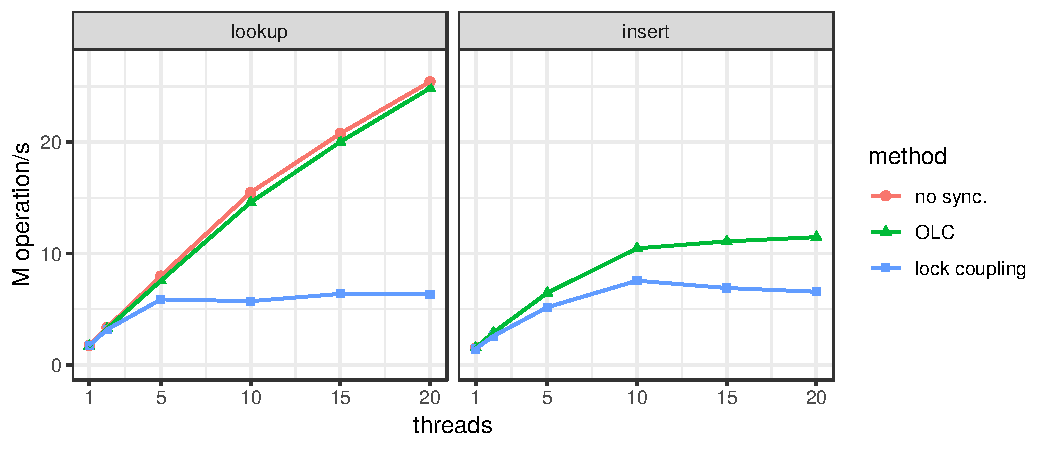
\includegraphics[width=\linewidth]{scale.pdf}
  \vspace{0.2cm}
  \caption{Scalability on 10-core system for B-tree operations (100M values).}
  \label{fig:scale}
\end{figure}

As Figure~\ref{fig:scale} shows, the results change dramatically once we use multiple threads.
For lookup, the scalability of OLC is near-linear up to 20 threads, even though the system has only 10 ``real cores''.
The OLC scalability for insert is also respectable (though not quite as linear because multi-threaded insertion approaches the memory bandwidth of our processor).
The figure also shows that the results of traditional lock coupling with read/write locks are significantly worse than OLC.
With 20 threads, lookup with OLC is 3.9$\times$ faster than traditional lock coupling.

\section{Summary}\label{sec:conc}

Optimistic Lock Coupling (OLC) is an effective synchronization method that combines the simplicity of traditional lock coupling with the superior scalability of lock-free approaches.
OLC is widely applicable and has already been successfully used to synchronize several data structures, including B-trees, binary search trees, and different trie variants.
These features make it highly attractive for modern database systems as well as performance-critical systems software in general.

\begin{thebibliography}{10}

\bibitem{DBLP:conf/spaa/BalmauGHZ16}
O.~Balmau, R.~Guerraoui, M.~Herlihy, and I.~Zablotchi.
\newblock Fast and robust memory reclamation for concurrent data structures.
\newblock In {\em SPAA}, 2016.

\bibitem{DBLP:journals/acta/BayerS77}
R.~Bayer and M.~Schkolnick.
\newblock Concurrency of operations on {B}-trees.
\newblock {\em Acta Informatica}, 9, 1977.

\bibitem{hot}
R.~Binna, E.~Zangerle, M.~Pichl, G.~Specht, and V.~Leis.
\newblock {HOT}: A height optimized trie index for main-memory database
  systems.
\newblock In {\em SIGMOD}, 2018.

\bibitem{DBLP:conf/ppopp/BronsonCCO10}
N.~G. Bronson, J.~Casper, H.~Chafi, and K.~Olukotun.
\newblock A practical concurrent binary search tree.
\newblock In {\em PPOPP}, 2010.

\bibitem{DBLP:conf/vldb/ChaHKK01}
S.~K. Cha, S.~Hwang, K.~Kim, and K.~Kwon.
\newblock Cache-conscious concurrency control of main-memory indexes on
  shared-memory multiprocessor systems.
\newblock In {\em VLDB}, 2001.

\bibitem{intel}
I.~Cutress.
\newblock {Intel} goes for 48-cores: {Cascade-AP} with multi-chip package
  coming soon.
\newblock
  \url{https://www.anandtech.com/show/13535/intel-goes-for-48cores-cascade-ap},
  2018 (accessed January, 2019).

\bibitem{DBLP:conf/cidr/FaleiroA17}
J.~M. Faleiro and D.~J. Abadi.
\newblock Latch-free synchronization in database systems: Silver bullet or
  fool's gold?
\newblock In {\em CIDR}, 2017.

\bibitem{DBLP:journals/ftdb/Graefe11}
G.~Graefe.
\newblock Modern {B}-tree techniques.
\newblock {\em Foundations and Trends in Databases}, 3(4), 2011.

\bibitem{DBLP:conf/hpca/KarnagelDRLLSL14}
T.~Karnagel, R.~Dementiev, R.~Rajwar, K.~Lai, T.~Legler, B.~Schlegel, and
  W.~Lehner.
\newblock Improving in-memory database index performance with
  {Intel}\({}^{\mbox{{\textregistered}}}\) transactional synchronization
  extensions.
\newblock In {\em HPCA}, 2014.

\bibitem{DBLP:journals/tods/LehmanY81}
P.~L. Lehman and S.~B. Yao.
\newblock Efficient locking for concurrent operations on {B}-trees.
\newblock {\em {ACM} Trans. Database Syst.}, 6(4), 1981.

\bibitem{leanstore}
V.~Leis, M.~Haubenschild, A.~Kemper, and T.~Neumann.
\newblock Leanstore: In-memory data management beyond main memory.
\newblock In {\em ICDE}, 2018.

\bibitem{art}
V.~Leis, A.~Kemper, and T.~Neumann.
\newblock The adaptive radix tree: {ARTful} indexing for main-memory databases.
\newblock In {\em ICDE}, 2013.

\bibitem{htmtkde}
V.~Leis, A.~Kemper, and T.~Neumann.
\newblock Scaling {HTM}-supported database transactions to many cores.
\newblock {\em {IEEE} Trans. Knowl. Data Eng.}, 28(2), 2016.

\bibitem{artsync}
V.~Leis, F.~Scheibner, A.~Kemper, and T.~Neumann.
\newblock The {ART} of practical synchronization.
\newblock In {\em DaMoN}, 2016.

\bibitem{DBLP:conf/icde/LevandoskiLS13a}
J.~J. Levandoski, D.~B. Lomet, and S.~Sengupta.
\newblock The {Bw}-tree: A {B}-tree for new hardware platforms.
\newblock In {\em ICDE}, 2013.

\bibitem{DBLP:journals/pvldb/MakreshanskiLS15}
D.~Makreshanski, J.~J. Levandoski, and R.~Stutsman.
\newblock To lock, swap, or elide: On the interplay of hardware transactional
  memory and lock-free indexing.
\newblock {\em {PVLDB}}, 8(11), 2015.

\bibitem{DBLP:dblp_conf/eurosys/MaoKM12}
Y.~Mao, E.~Kohler, and R.~T. Morris.
\newblock Cache craftiness for fast multicore key-value storage.
\newblock In {\em EuroSys}, 2012.

\bibitem{DBLP:journals/tpds/Michael04}
M.~M. Michael.
\newblock Hazard pointers: Safe memory reclamation for lock-free objects.
\newblock {\em {IEEE} Trans. Parallel Distrib. Syst.}, 15(6), 2004.

\bibitem{DBLP:journals/jacm/ShalevS06}
O.~Shalev and N.~Shavit.
\newblock Split-ordered lists: Lock-free extensible hash tables.
\newblock {\em J. {ACM}}, 53(3), 2006.

\bibitem{amd}
A.~Shilov.
\newblock {AMD} previews {EPYC} ‘{Rome}’ processor: Up to 64 {Zen} 2 cores.
\newblock
  \url{https://www.anandtech.com/show/13561/amd-previews-epyc-rome-processor-up-to-64-zen-2-cores},
  2018 (accessed January, 2019).

\bibitem{DBLP:conf/sosp/TuZKLM13}
S.~Tu, W.~Zheng, E.~Kohler, B.~Liskov, and S.~Madden.
\newblock Speedy transactions in multicore in-memory databases.
\newblock In {\em SOSP}, 2013.

\bibitem{buzzword}
Z.~Wang, A.~Pavlo, H.~Lim, V.~Leis, H.~Zhang, M.~Kaminsky, and D.~Andersen.
\newblock Building a {Bw}-tree takes more than just buzz words.
\newblock In {\em SIGMOD}, 2018.

\end{thebibliography}


%\bibliographystyle{abbrv}
%\bibliography{main}

\end{document}

\end{article}


\begin{article}
{Distilling Causal Metaknowledge from Knowledge Graphs}
{Yuan Meng, Yancheng Dong, Shixuan Liu, Chaohao Yuan, Yue He, Jian Pei, and Peng Cui}
\pdfminorversion=5
\documentclass[11pt]{article}
\usepackage{deauthor,times,graphicx,caption,microtype}
\usepackage{hyperref}
\usepackage{listings}
\usepackage{booktabs}

\begin{document}

\title{Optimistic Lock Coupling: A Scalable and Efficient General-Purpose Synchronization Method}

\author{Viktor Leis, Michael Haubenschild\raisebox{0.9ex}{$\ast$}, Thomas Neumann\\ Technische Universit{\"a}t M{\"u}nchen \hspace{0.7cm} Tableau Software\raisebox{0.9ex}{$\ast$} \\ {\{leis,neumann\}{@}in.tum.de} \hspace{0.7cm} {mhaubenschild{@}tableau.com\raisebox{0.9ex}{$\ast$}}}

\maketitle

\begin{abstract}
As the number of cores on commodity processors continues to increase, scalability becomes more and more crucial for overall performance.
Scalable and efficient concurrent data structures are particularly important, as these are often the building blocks of parallel algorithms.
Unfortunately, traditional synchronization techniques based on fine-grained locking have been shown to be unscalable on modern multi-core CPUs.
Lock-free data structures, on the other hand, are extremely difficult to design and often incur significant overhead.

In this work, we make the case for Optimistic Lock Coupling as a practical alternative to both traditional locking and the lock-free approach.
We show that Optimistic Lock Coupling is highly scalable and almost as simple to implement as traditional lock coupling.
Another important advantage is that it is easily applicable to most tree-like data structures.
We therefore argue that Optimistic Lock Coupling, rather than a complex and error-prone custom synchronization protocol, should be the default choice for performance-critical data structures.
\end{abstract}

\section{Introduction}

% more and more cores
Today, Intel's commodity server processors have up to 28 cores and its upcoming microarchitecture will have up to 48 cores per socket~\cite{intel}.
Similarly, AMD currently stands at 32 cores and this number is expected to double in the next generation~\cite{amd}.
Since both platforms support simultaneous multithreading (also known as hyperthreading), affordable commodity servers (with up to two sockets) will soon routinely have between 100 and 200 hardware threads.

% data structure scalability is important
With such a high degree of hardware parallelism, efficient data processing crucially depends on how well concurrent data structures scale.
Internally, database systems use a plethora of data structures like table heaps, internal work queues, and, most importantly, index structures.
Any of these can easily become a scalability (and therefore overall performance) bottleneck on many-core CPUs.

% traditional synchronization: fine-grained locks, slow, cache invalidation
Traditionally, database systems synchronize internal data structures using fine-grained reader/writer locks\footnote{In this work, we focus on data structure synchronization rather than high-level transaction semantics and therefore use the term {\em lock} for what would typically be called {\em latch} in the database literature. We thus follow common computer science (rather than database) terminology.}.
Unfortunately, while fine-grained locking makes lock contention unlikely, it still results in bad scalability because lock acquisition and release require writing to shared memory.
Due to the way cache coherency is implemented on modern multi-core CPUs, these writes cause additional cache misses\footnote{The cache coherency protocol ensures that all copies of a cache line on other cores are invalidated before the write can proceed.} and the cache line containing the lock's internal data becomes a point of physical contention.
As a result, any frequently-accessed lock (e.g., the lock of the root node of a B-tree) severely limits scalability.

% lock-free bw-tree: no more latches, but indirections, extremely complex
Lock-free data structures like the Bw-tree~\cite{DBLP:conf/icde/LevandoskiLS13a} (a lock-free B-tree variant) or the Split-Ordered List~\cite{DBLP:journals/jacm/ShalevS06} (a lock-free hash table) do not acquire any locks and therefore generally scale much better than locking-based approaches (in particular for read-mostly workloads).
However, lock-free synchronization has other downsides:
First, it is very difficult and results in extremely complex and error-prone code (when compared to locking).
Second, because the functionality of atomic primitives provided by the hardware (e.g., atomically compare-and-swap 8 bytes) is limited, complex operations require additional indirections within the data structure.
For example, the Bw-tree requires an indirection table and the Split-Ordered List requires ``dummy nodes'', resulting in overhead due to additional cache misses.

% OLC for the win
In this paper we make the case for {\em Optimistic Lock Coupling (OLC)}, a synchronization method that combines some of the best properties of lock-based and lock-free synchronization.
OLC utilizes a special lock type that can be used in two modes:
The first mode is similar to a traditional mutex and excludes other threads by physically acquiring the underlying lock.
In the second mode, reads can proceed optimistically by validating a version counter that is embedded in the lock (similar to optimistic concurrency control).
The first mode is typically used by writers and the second mode by readers.
Besides this special lock type, OLC is based on the observation that optimistic lock validations can be interleaved/coupled---similar to the pair-wise interleaved lock acquisition of traditional lock coupling.
Hence, the name Optimistic Lock Coupling.

OLC has a number of desirable features:
\begin{itemize}
\item By reducing the number of writes to shared memory locations and thereby avoiding cache invalidations, it {\bf scales well} for most workloads.
\item In comparison to unsynchronized code, it requires few additional CPU instructions making it {\bf efficient}.
\item OLC is {\bf widely applicable} to different data structures. It has already been successfully used for synchronizing binary search trees~\cite{DBLP:conf/ppopp/BronsonCCO10}, tries~\cite{artsync}, trie/B-tree hybrids~\cite{DBLP:dblp_conf/eurosys/MaoKM12}, and B-trees~\cite{buzzword}.
\item In comparison to the lock-free paradigm, it is also {\bf easy to use} and requires few modifications to existing, single-threaded data structures.
\end{itemize}
Despite these positive features and its simplicity, OLC is not yet widely known.
The goal of this paper is therefore to popularize this simple idea and to make a case for it.
We argue that OLC deserves to be widely known.
It is a good default synchronization paradigm---more complex, data structure-specific protocols are seldom beneficial.

The rest of the paper is organized as follows.
Section~\ref{sec:related} discusses related work, tracing the history of OLC and its underlying ideas in the literature.
The core of the paper is Section~\ref{sec:olc}, which describes the ideas behind OLC and how it can be used to synchronize complex data structures.
In Section~\ref{sec:evaluation} we experimentally show that OLC has low overhead and scales well when used to synchronize an in-memory B-tree.
We summarize the paper in Section~\ref{sec:conc}.

\newpage
\section{Related Work}\label{sec:related}

Lock coupling has been proposed as a method for allowing concurrent operations on B-trees in 1977~\cite{DBLP:journals/acta/BayerS77}.
This traditional and still widely-used method, described in detail in Graefe's B-tree survey~\cite{DBLP:journals/ftdb/Graefe11}, is also called ``latch coupling'', ``hand-over-hand locking'', and ``crabbing''.
Because at most two locks are held at-a-time during tree traversal, this technique seemingly allows for a high degree of parallelism---in particular if read/write locks are used to enable inner nodes to be locked in shared mode.
However, as we show in Section~\ref{sec:evaluation}, on modern hardware lock acquisition (even in shared mode) results in suboptimal scalability.

An early alternative from 1981 is a B-tree variant called B-link tree~\cite{DBLP:journals/tods/LehmanY81}, which only holds a single lock at a time.
It is based on the observation that between the release of the parent lock and the acquisition of the child lock, the only ``dangerous'' thing that could have happened is the split of a child node (assuming one does not implement merge operations).
Thus, when a split happens, the key being searched might end up on a neighboring node to the right of the current child node.
A B-link tree traversal therefore detects this condition and, if needed, transparently proceeds to the neighboring node.
Releasing the parent lock early is highly beneficial when the child node needs to be fetched from disk.
For in-memory workloads, however, the B-link tree has the same scalability issues as lock coupling (it acquires just as many locks).

The next major advance, Optimistic Latch-Free Index Traversal (OLFIT)~\cite{DBLP:conf/vldb/ChaHKK01}, was proposed in 2001.
OLFIT introduced the idea of a combined lock/update counter, which we call {\em optimistic lock}. % , for lack of a better name,
Based on these per-node optimistic locks and the synchronization protocol of the B-link tree, OLFIT finally achieves good scalability on parallel processors.
The OLFIT protocol is fairly complex, as it requires both the non-trivial B-link protocol and optimistic locks.
Furthermore, like the B-link tree protocol, it does not support merging nodes, and is specific to B-trees (cannot easily be applied to other data structures).

In the following two decades, the growth of main-memory capacity led to much research into other data structures besides the venerable B-tree.
Particularly relevant for our discussion is Bronson et al.'s~\cite{DBLP:conf/ppopp/BronsonCCO10} concurrent binary search tree, which is based on optimistic version validation and has a sophisticated, data structure-specific synchronization protocol.
To the best of our knowledge, this 2010 paper is the first that, as part of its protocol, interleaves version validation across nodes---rather than validating each node separately like OLFIT.
In that paper, this idea is called ``hand-over-hand, optimistic validation'', while we prefer the term Optimistic Lock Coupling to highlight the close resemblance to traditional lock coupling.
Similarly, Mao et al.'s~\cite{DBLP:dblp_conf/eurosys/MaoKM12} Masstree (a concurrent hybrid trie/B-tree) is also based on the same ideas, but again uses them as part of a more complex protocol.

The Adaptive Radix Tree (ART)~\cite{art} is another recent in-memory data structure, which we proposed in 2013.
In contrast to the two data structures just mentioned, it was originally designed with single-threaded performance in mind without supporting concurrency.
To add support for concurrency, we initially started designing a custom protocol called Read-Optimized Write Exclusion (ROWEX)~\cite{artsync}, which turned out to be non-trivial and requires modifications of the underlying data structure\footnote{Note that ROWEX is already easier to apply to existing data structures than the lock-free approach. The difficulty depends on the data structure. Applying ROWEX is hard for B-trees with sorted keys and fairly easy for copy-on-write data structures like the Height Optimized Trie~\cite{hot}---with ART being somewhere in the middle.}.
However, fairly late in the project, we also realized, that OLC {\em alone} (rather than as part of a more complex protocol) is sufficient to synchronize ART.
No other changes to the data structure were necessary.
Both approaches were published and experimentally evaluated in a followup paper~\cite{artsync}, which shows that, despite its simplicity, OLC is efficient, scalable, and generally outperforms ROWEX.

Similar results were recently published regarding B-trees~\cite{buzzword}.
In this experimental study a simple OLC-based synchronization outperformed the Bw-tree~\cite{DBLP:conf/icde/LevandoskiLS13a}, a complex lock-free synchronization approach.
Another recent paper shows that for write-intensive workloads, locking often performs better than lock-free synchronization~\cite{DBLP:conf/cidr/FaleiroA17}.
These experiences indicate that OLC is a general-purpose synchronization paradigm and motivate the current paper.

%foster b-tree\cite{DBLP:journals/tods/GraefeKK12}
%Shasha theory~\cite{DBLP:journals/tods/ShashaG88}

\section{Optimistic Lock Coupling}\label{sec:olc}

% locks suck
The standard technique for inter-thread synchronization is mutual exclusion using fine-grained locks.
In a B-tree, for example, every node usually has its own associated lock, which is acquired before accessing that node.
The problem of locking on modern multi- and many-core processors is that lock acquisition and release require writing to the shared memory location that implements the lock.
This write causes exclusive ownership of the underlying cache line and invalidates copies of it on all other processor cores.
For hierarchical, tree-like data structures, the lock of the root node becomes a point of physical contention---even in read-only workloads and even when read/write locks are used.
Depending on the specific data structure, number of cores, cache coherency protocol implementation, cache topology, whether Non-Uniform Memory Access (NUMA) is used, locking can even result in multi-threaded performance that is worse than single-threaded execution.

% in b-trees this happens very much
The inherent pessimism of locking is particularly unfortunate for B-trees:
Despite the fact that logical modifications of the root node are very infrequent, every B-tree operation must lock the root node during tree traversal\footnote{To a lesser extent this obviously applies to all inner nodes, not just the root.}.
Even the vast majority of update operations (with the exception of splits and merges), only modify a single leaf node.
These observations indicate that a more optimistic approach, which does not require locking inner nodes, would be very beneficial for B-trees.

\subsection{Optimistic Locks}

% optimism to the rescue
As the name indicates, optimistic locks try to solve the scalability issues of traditional locks using an optimistic approach.
Instead of always physically acquiring locks, even for nodes that are unlikely to be modified simultaneously, after-the-fact validation is used to detect conflicts.
This is done by augmenting each lock with a version/update counter that is incremented on every modification.
Using this version counter, readers can optimistically proceed before validating that the version did not change to ensure that the read was safe.
If validation fails, the operation is restarted.

% details on opt locks
Using optimistic locks, a read-only node access (i.e., the majority of all operations in a B-tree) does not acquire the lock and does not increment the version counter.
Instead, it performs the following steps:
\begin{enumerate}
\item read lock version (restart if lock is not free)
\item access node
\item read the version again and validate that it has not changed in the meantime
\end{enumerate}
If the last step (the validation) fails, the operation has to be restarted.
Write operations, on the other hand, are more similar to traditional locking:
\begin{enumerate}
\item acquire lock (wait if necessary)
\item access/write to node
\item increment version and unlock node
\end{enumerate}
Writes can therefore protect a node from other writes.

% similar to locks
As we observed in an earlier paper~\cite{artsync}, because of similar semantics, optimistic locks can be hidden behind an API very similar to traditional read/write locks.
Both approaches have an exclusive lock mode, and acquiring a traditional lock in shared mode is analogous to optimistic version validation.
Furthermore, like with some implementations of traditional read/write locks, optimistic locks allow upgrading a shared lock to an exclusive lock.
Lock upgrades are, for example, used to avoid most B-tree update operations from having to lock inner nodes.
In our experience, the close resemblance of optimistic and traditional locks simplifies the reasoning about optimistic locks;
one can apply similar thinking as in traditional lock-based protocols.

\subsection{Lock Coupling with Optimistic Locks}

\begin{figure}
  \centering
  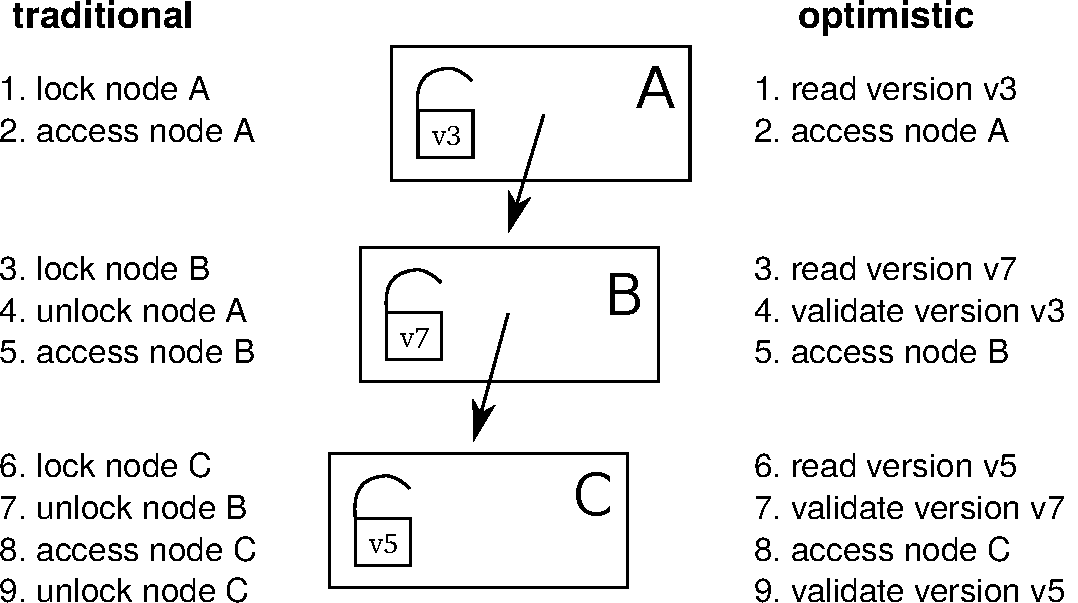
\includegraphics[width=0.65\linewidth]{olcall.pdf}
  \vspace{0.2cm}
  \caption{Comparison of a lookup operation in a 3-level tree using traditional lock coupling (left-hand side) vs.~optimistic lock coupling (right-hand side).}
  \label{fig:olc}
\end{figure}

The traditional and most common lock-based synchronization protocol for B-trees is lock coupling, which interleaves lock acquisitions while holding at most two locks at a time.
If, as we observed earlier, optimistic locks have similar semantics as traditional locks, it is natural to ask whether lock coupling can be combined with optimistic locks.
And indeed the answer is yes: One can almost mechanically translate traditional lock coupling code to optimistic lock coupling code.
This is illustrated in Figure~\ref{fig:olc}, which compares the traversal in a tree of height 3 using traditional and optimistic locks.
As the figure shows, the main difference is that locking is translated to reading the version and that unlocking becomes validation of the previously read version.
This simple change provides efficient lock-free tree traversal without the need to design a complex synchronization protocol.

It is important to emphasize the conceptual simplicity of OLC in comparison to data structures that use custom protocols like the Bw-tree~\cite{DBLP:conf/icde/LevandoskiLS13a}.
To implement lock-free access, the Bw-tree requires an indirection table, delta nodes, complex splitting and merging logic, retry logic, etc.
OLC, on the other hand, can directly be applied to B-trees mostly by adding the appropriate optimistic locking code and without modifying the node layout itself.
Therefore, OpenBw-Tree, an open source implementation of the Bw-tree, requires an order of magnitude more code than a B-tree based on OLC\footnote{Both implementations are available on GitHub: \url{https://github.com/wangziqi2016/index-microbench}}.
Given how difficult it is to develop, validate, and debug lock-free code, simplicity is obviously a major advantage.

\subsection{Correctness Aspects}

\begin{figure}
  % \centering
  %[basicstyle=\normalsize\ttfamily,showstringspaces=false,columns=fullflexible,breaklines=false,breakatwhitespace=true,numbers=none,numberstyle=\small,style=C,keepspaces=true]
\begin{lstlisting}[basicstyle=\ttfamily,language=C++,numbers=left,numberstyle=\small]
std::atomic<BTreeNode*> root;

// search for key in B+tree, returns payload in resultOut
bool lookup(Key key, Value& resultOut) {
   BTreeNode* node = root.load();
   uint64_t nodeVersion = node->readLockOrRestart();
   if (node != root.load()) // make sure the root is still the root
      restart();

   BTreeInner<Key>* parent = nullptr;
   uint64_t parentVersion = 0;

   while (node->isInner()) {
      auto inner = (BTreeInner*)node;

      // unlock parent and make current node the parent
      if (parent)
         parent->readUnlockOrRestart(parentVersion);
      parent = inner;
      parentVersion = nodeVersion;

      // search for next node
      node = inner->findChild(key);
      // validate 'inner' to ensure that 'node' pointer is valid
      inner->checkOrRestart(nodeVersion);
      // now it safe to dereference 'node' pointer (read its version)
      nodeVersion = node->readLockOrRestart();
   }

   // search in leaf and retrieve payload
   auto leaf = (BTreeLeaf*)node;
   bool success = leaf->findValue(key, resultOut);

   // unlock everything
   if (parent)
      parent->readUnlockOrRestart(parentVersion);
   node->readUnlockOrRestart(nodeVersion);

   return success;
}
\end{lstlisting}
  \vspace{0.2cm}
  \caption{B-tree lookup code using OLC. For simplicity, the restart logic is not shown.}
  \label{fig:lookup}
\end{figure}

So far, we have introduced the high-level ideas behind OLC and have stressed its similarity to traditional lock coupling.
Let us now discuss some cases where the close similarity between lock coupling and OLC breaks down.
To make this more concrete, we show the B-tree lookup code in Figure~\ref{fig:lookup}.
In the code, \texttt{readLockOrRestart} reads the lock version and \texttt{readUnlockOrRestart} validates that the read was correct.

One issue with OLC is that any pointer speculatively read from a node may point to invalid memory (if that node is modified concurrently).
Dereferencing such a pointer (e.g., to read its optimistic lock), may cause a segmentation fault or undefined behavior.
In the code shown in Figure~\ref{fig:lookup}, this problem is prevented by the extra check in line 25, which ensures that the read from the node containing the pointer was correct.
Without this additional validation, the code would in line 27 dereference the pointer speculatively read in line 23.
Note that the implementation of \texttt{checkOrRestart} is actually identical to \texttt{readUnlockOrRestart}.
We chose to give it a different name to highlight the fact that this extra check would not be necessary with read/write locks.

Another potential issue with optimistic locks is code that does not terminate.
Code that speculatively accesses a node, like an intra-node binary search, should be written in a way such that it always terminates---even in the presence of concurrent writes.
Otherwise, the validation code that detects the concurrent write will never run.
The binary search of a B-tree, for example, needs to be written in such a way that each comparison makes progress.
For some data structures that do not require loops in the traversal code (like ART) termination is trivially true.

\subsection{Implementation Details}

% implementation, efficiency
To implement an optimistic lock, one can combine the lock and the version counter into a single 64-bit\footnote{Even after subtracting one bit for the lock status, a back-of-the-envelope calculation can show that 63 bits are large enough to never overflow in practice.} word~\cite{artsync}.
A typical read operation will therefore merely consist of reading this version counter atomically.
In C++11 this can be implemented using the \texttt{std::atomic} type.

On x86, atomic reads are cheap because of x86's strong memory order guarantees.
No memory fences are required for sequentially-consistent loads, which are translated (by both GCC and clang) into standard \texttt{MOV} instructions.
Hence, the only effect of \texttt{std::atomic} for loads is preventing instruction re-ordering.
This makes version access and validation cheap.
Acquiring and releasing an optimistic lock in exclusive mode has comparable cost to a traditional lock:
A fairly expensive sequentially-consistent store is needed for acquiring a lock, while a standard \texttt{MOV} suffices for releasing it.
A simple sinlock-based implementation of optimistic locks can be found in the appendix of an earlier paper~\cite{artsync}.

OLC code must be able to handle restarts since validation or lock upgrade can fail due to concurrent writers.
Restarts can easily be implemented by wrapping the data structure operation in a loop (for simplicity not shown in Figure~\ref{fig:lookup}).
Such a loop also enables limiting the number of optimistic retry operations and falling back to pessimistic locking in cases of very heavy contention.
The ability to fall back to traditional locking is a major advantage of OLC in terms of robustness over lock-free approaches, which do not have this option.

In addition to the optimistic shared mode and the exclusive mode, optimistic locks also support a ``shared pessimistic'' mode, which physically acquires the lock in shared mode (allowing multiple concurrent readers but no writers).
This mode is useful for table (or range) scans that touch many tuples on a leaf page (which would otherwise easily abort).
Finally, let us mention that large range scans and table scans, should be broken up into several per-node traversals as is done in the LeanStore~\cite{leanstore} system.

Like all lock-free data structures, but unlike traditional locking and Hardware Transactional Memory~\cite{DBLP:conf/hpca/KarnagelDRLLSL14,DBLP:journals/pvldb/MakreshanskiLS15,htmtkde}, OLC requires care when deleting (and reusing) nodes.
The reason is that a deleting thread can never be sure that a node can be reclaimed because other threads might still be optimistically reading from that node.
Therefore, standard solutions like epoch-based reclamation~\cite{DBLP:conf/sosp/TuZKLM13}, hazard pointers~\cite{DBLP:journals/tpds/Michael04}, or optimized hazard pointers~\cite{DBLP:conf/spaa/BalmauGHZ16} need to be used.
These memory reclamation techniques are, however, largely orthogonal to the synchronization protocol itself.

%-lock-free is not a strong guarantee

\newpage
\section{Evaluation}\label{sec:evaluation}

Let us now experimentally evaluate the overhead and scalability of OLC.
For the experiments, we use an in-memory B+tree implemented in C++11 using templates, which is configured to use nodes of 4096 bytes, random 8 byte keys, and 8 byte payloads.
Based on this B-tree, we compare the following synchronization approaches:
\begin{itemize}
\item an OLC implementation\footnote{An almost identical OLC implementation is available on github: \url{https://github.com/wangziqi2016/index-microbench/tree/master/BTreeOLC}}
\item a variant based on traditional lock coupling and read/write locks
\item the unsynchronized B-tree, which obviously is only correct for read-only workloads but allows measuring the overhead of synchronization
\end{itemize}
Note that earlier work has compared the OLC implementation with a Bw-tree implementation~\cite{buzzword} and other state-of-the-art in-memory index structures.

We use a Haswell EP system with an Intel Xeon E5-2687W v3 CPU, which has 10 cores (20 ``Hyper-Threads'') and 25~MB of L3 cache.
The system is running Ubuntu 18.10 and we use GCC 8.2.0 to compile our code.
The CPU counters are obtained using the Linux perf API\footnote{We use the following convenience wrapper: \url{https://github.com/viktorleis/perfevent}}.

\begin{table}
  \caption{Performance and CPU counters for lookup and insert operations in a B-tree with 100M keys. We perform 100M operations and normalize the CPU counters by that number.}
  \label{tab:overhead}
  \centering
  \begin{tabular}{lrrrrrrr}\toprule
                    &         &        &        & instruc-  & L1     & L3     & branch \\
                    & threads & M op/s & cycles & tions & misses & misses & misses \\\midrule
lookup (no sync.)   & 1       & 1.72   & 2028   & 283     & 39.1   & 14.9   & 16.1   \\
lookup (OLC)        & 1       & 1.65   & 2107   & 370     & 43.9   & 15.1   & 16.7   \\
lookup (lock coup.) & 1       & 1.72   & 2078   & 365     & 42.3   & 16.9   & 15.7   \\\midrule
insert (no sync.)   & 1       & 1.51   & 2286   & 530     & 59.8   & 31.1   & 17.3   \\
insert (OLC)        & 1       & 1.50   & 2303   & 629     & 61.2   & 31.1   & 16.5   \\
insert (lock coup.) & 1       & 1.41   & 2473   & 644     & 61.0   & 31.0   & 17.2   \\\midrule
lookup (no sync.)   & 10      & 15.48  & 2058   & 283     & 38.6   & 15.5   & 16.0   \\
lookup (OLC)        & 10      & 14.60  & 2187   & 370     & 43.8   & 15.8   & 16.8   \\
lookup (lock coup.) & 10      & 5.71   & 5591   & 379     & 54.2   & 17.0   & 14.8   \\\midrule
insert (no sync.)   & 10      & -      & -      & -       & -      & -      & -      \\
insert (OLC)        & 10      & 10.46  & 2940   & 656     & 62.0   & 32.5   & 16.8   \\
insert (lock coup.) & 10      & 7.55   & 4161   & 667     & 75.0   & 28.6   & 16.2   \\
    \bottomrule
\end{tabular}
\end{table}

Table~\ref{tab:overhead} compares the performance and CPU counters for lookup and insert operations in a B-tree with 100M keys.
With {\em single-threaded} execution, we observe that all three approaches have very similar performance.
Adding traditional or optimistic locks to unsynchronized B-tree code results in up to 30\% of additional instructions without affecting single-threaded performance much.

\begin{figure}
  \centering
  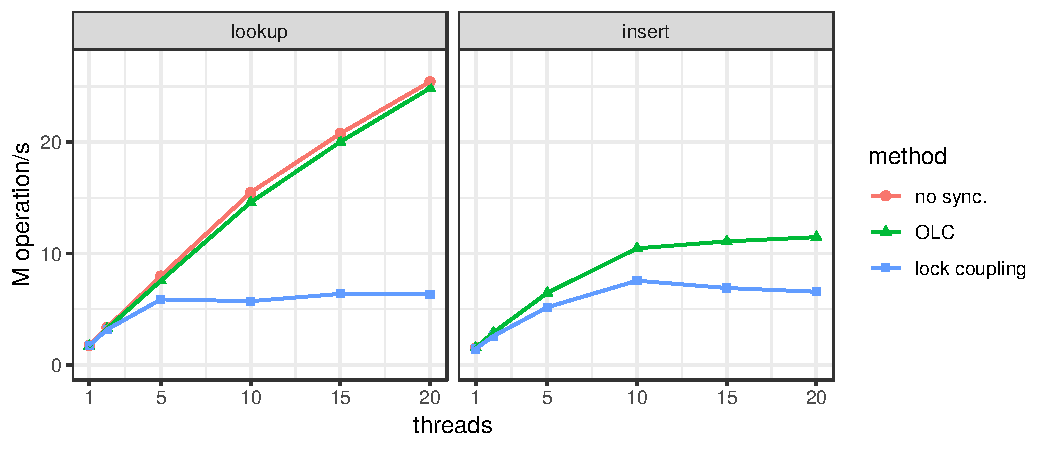
\includegraphics[width=\linewidth]{scale.pdf}
  \vspace{0.2cm}
  \caption{Scalability on 10-core system for B-tree operations (100M values).}
  \label{fig:scale}
\end{figure}

As Figure~\ref{fig:scale} shows, the results change dramatically once we use multiple threads.
For lookup, the scalability of OLC is near-linear up to 20 threads, even though the system has only 10 ``real cores''.
The OLC scalability for insert is also respectable (though not quite as linear because multi-threaded insertion approaches the memory bandwidth of our processor).
The figure also shows that the results of traditional lock coupling with read/write locks are significantly worse than OLC.
With 20 threads, lookup with OLC is 3.9$\times$ faster than traditional lock coupling.

\section{Summary}\label{sec:conc}

Optimistic Lock Coupling (OLC) is an effective synchronization method that combines the simplicity of traditional lock coupling with the superior scalability of lock-free approaches.
OLC is widely applicable and has already been successfully used to synchronize several data structures, including B-trees, binary search trees, and different trie variants.
These features make it highly attractive for modern database systems as well as performance-critical systems software in general.

\begin{thebibliography}{10}

\bibitem{DBLP:conf/spaa/BalmauGHZ16}
O.~Balmau, R.~Guerraoui, M.~Herlihy, and I.~Zablotchi.
\newblock Fast and robust memory reclamation for concurrent data structures.
\newblock In {\em SPAA}, 2016.

\bibitem{DBLP:journals/acta/BayerS77}
R.~Bayer and M.~Schkolnick.
\newblock Concurrency of operations on {B}-trees.
\newblock {\em Acta Informatica}, 9, 1977.

\bibitem{hot}
R.~Binna, E.~Zangerle, M.~Pichl, G.~Specht, and V.~Leis.
\newblock {HOT}: A height optimized trie index for main-memory database
  systems.
\newblock In {\em SIGMOD}, 2018.

\bibitem{DBLP:conf/ppopp/BronsonCCO10}
N.~G. Bronson, J.~Casper, H.~Chafi, and K.~Olukotun.
\newblock A practical concurrent binary search tree.
\newblock In {\em PPOPP}, 2010.

\bibitem{DBLP:conf/vldb/ChaHKK01}
S.~K. Cha, S.~Hwang, K.~Kim, and K.~Kwon.
\newblock Cache-conscious concurrency control of main-memory indexes on
  shared-memory multiprocessor systems.
\newblock In {\em VLDB}, 2001.

\bibitem{intel}
I.~Cutress.
\newblock {Intel} goes for 48-cores: {Cascade-AP} with multi-chip package
  coming soon.
\newblock
  \url{https://www.anandtech.com/show/13535/intel-goes-for-48cores-cascade-ap},
  2018 (accessed January, 2019).

\bibitem{DBLP:conf/cidr/FaleiroA17}
J.~M. Faleiro and D.~J. Abadi.
\newblock Latch-free synchronization in database systems: Silver bullet or
  fool's gold?
\newblock In {\em CIDR}, 2017.

\bibitem{DBLP:journals/ftdb/Graefe11}
G.~Graefe.
\newblock Modern {B}-tree techniques.
\newblock {\em Foundations and Trends in Databases}, 3(4), 2011.

\bibitem{DBLP:conf/hpca/KarnagelDRLLSL14}
T.~Karnagel, R.~Dementiev, R.~Rajwar, K.~Lai, T.~Legler, B.~Schlegel, and
  W.~Lehner.
\newblock Improving in-memory database index performance with
  {Intel}\({}^{\mbox{{\textregistered}}}\) transactional synchronization
  extensions.
\newblock In {\em HPCA}, 2014.

\bibitem{DBLP:journals/tods/LehmanY81}
P.~L. Lehman and S.~B. Yao.
\newblock Efficient locking for concurrent operations on {B}-trees.
\newblock {\em {ACM} Trans. Database Syst.}, 6(4), 1981.

\bibitem{leanstore}
V.~Leis, M.~Haubenschild, A.~Kemper, and T.~Neumann.
\newblock Leanstore: In-memory data management beyond main memory.
\newblock In {\em ICDE}, 2018.

\bibitem{art}
V.~Leis, A.~Kemper, and T.~Neumann.
\newblock The adaptive radix tree: {ARTful} indexing for main-memory databases.
\newblock In {\em ICDE}, 2013.

\bibitem{htmtkde}
V.~Leis, A.~Kemper, and T.~Neumann.
\newblock Scaling {HTM}-supported database transactions to many cores.
\newblock {\em {IEEE} Trans. Knowl. Data Eng.}, 28(2), 2016.

\bibitem{artsync}
V.~Leis, F.~Scheibner, A.~Kemper, and T.~Neumann.
\newblock The {ART} of practical synchronization.
\newblock In {\em DaMoN}, 2016.

\bibitem{DBLP:conf/icde/LevandoskiLS13a}
J.~J. Levandoski, D.~B. Lomet, and S.~Sengupta.
\newblock The {Bw}-tree: A {B}-tree for new hardware platforms.
\newblock In {\em ICDE}, 2013.

\bibitem{DBLP:journals/pvldb/MakreshanskiLS15}
D.~Makreshanski, J.~J. Levandoski, and R.~Stutsman.
\newblock To lock, swap, or elide: On the interplay of hardware transactional
  memory and lock-free indexing.
\newblock {\em {PVLDB}}, 8(11), 2015.

\bibitem{DBLP:dblp_conf/eurosys/MaoKM12}
Y.~Mao, E.~Kohler, and R.~T. Morris.
\newblock Cache craftiness for fast multicore key-value storage.
\newblock In {\em EuroSys}, 2012.

\bibitem{DBLP:journals/tpds/Michael04}
M.~M. Michael.
\newblock Hazard pointers: Safe memory reclamation for lock-free objects.
\newblock {\em {IEEE} Trans. Parallel Distrib. Syst.}, 15(6), 2004.

\bibitem{DBLP:journals/jacm/ShalevS06}
O.~Shalev and N.~Shavit.
\newblock Split-ordered lists: Lock-free extensible hash tables.
\newblock {\em J. {ACM}}, 53(3), 2006.

\bibitem{amd}
A.~Shilov.
\newblock {AMD} previews {EPYC} ‘{Rome}’ processor: Up to 64 {Zen} 2 cores.
\newblock
  \url{https://www.anandtech.com/show/13561/amd-previews-epyc-rome-processor-up-to-64-zen-2-cores},
  2018 (accessed January, 2019).

\bibitem{DBLP:conf/sosp/TuZKLM13}
S.~Tu, W.~Zheng, E.~Kohler, B.~Liskov, and S.~Madden.
\newblock Speedy transactions in multicore in-memory databases.
\newblock In {\em SOSP}, 2013.

\bibitem{buzzword}
Z.~Wang, A.~Pavlo, H.~Lim, V.~Leis, H.~Zhang, M.~Kaminsky, and D.~Andersen.
\newblock Building a {Bw}-tree takes more than just buzz words.
\newblock In {\em SIGMOD}, 2018.

\end{thebibliography}


%\bibliographystyle{abbrv}
%\bibliography{main}

\end{document}

\end{article}



\end{articlesection}

% put the news items below- there can be multiple news sections
% each with its own title
% news will usually have an author as well as a title,
% e.g. TCDE elections
% news articles are in the same format as letters
% typically, news articles will be stored in a directory called "news"

%\begin{newssection}{News headline}

% insert news items here; news will typically have authors
% see the Sept. 2018 issue for an example

%\begin{news}{news item title}
%{author name}{author affiliation}
%\input{news/news-article.tex}
%\end{news}
%
%\newpage


%\end{newssection}

\begin{callsection}

%  This section will be empty for your version
%
%  Calls for papers section.  Use the callsection environment.
%  Each call for papers is contained in an call environment, where the single
%  required options to \begin{call} is the name of the conference.
% typically calls are stored in a "calls" directory
%
%\begin{call}{name of conference}
%\centerline{\includegraphics[width=\textwidth, bb= 0 0 590 760]{calls/conference-name.pdf}}
%\end{call}
%\begin{call}{ICDE 2019 Conference}
%\centerline{
\includegraphics[width=\textwidth, bb= 0 0 610 790] {../Dec-2018/calls/icde19.pdf}}
%\centerline{
\includegraphics[width=\textwidth, bb= 0 0 590 760] {calls/icde19.pdf}}
%\end{call}
\begin{call}{TCDE Membership Form}
%\centerline{\includegraphics[width=\textwidth, bb= 0 0 610 790]
%\centerline{
\includegraphics[width=\textwidth, bb= 0 0 590 760] {../Dec-2018/calls/tcde.pdf}}
\centerline{
\includegraphics[width=\textwidth, bb= 0 0 590 760] {../2020-09/calls/tcde.pdf}}
\end{call}

\end{callsection}

\end{bulletin}
\end{document}
